% !TEX root = ../proyect.tex

\chapter{Manual de Usuario}\label{cap09}

\section{Introducci\'on}\label{sec:manual-intro}

BargAIn permite al usuario gestionar su compra diaria desde una app m\'ovil (iOS y Android) y un
portal web para PYMEs, comparar precios entre supermercados cercanos, y calcular la ruta de compra
m\'as eficiente seg\'un sus preferencias de precio, distancia y tiempo.

\section{Requisitos de uso}\label{sec:manual-requisitos}

\begin{itemize}
  \item Dispositivo m\'ovil iOS (14+) o Android (10+) con la app instalada, o navegador web
    moderno para el portal business.
  \item Conexi\'on a Internet.
  \item Cuenta de usuario registrada en el sistema.
  \item Permisos de ubicaci\'on concedidos a la app (para funciones de mapa y optimizaci\'on).
\end{itemize}

Para el entorno de desarrollo local:
\begin{itemize}
  \item Backend levantado en Docker (\texttt{make dev}).
  \item Base de datos migrada (\texttt{make migrate-docker}).
  \item Frontend Expo en host (\texttt{make frontend}).
\end{itemize}

\section{Flujo de acceso}\label{sec:manual-acceso}

\begin{enumerate}
  \item Abrir la app en Expo/Web.
  \item Seleccionar ``Iniciar sesi\'on'' o ``Registrarse''.
  \item Introducir credenciales v\'alidas.
  \item Tras autenticaci\'on, se carga la navegaci\'on principal por pesta\~nas.
\end{enumerate}

El sistema usa JWT con refresco autom\'atico. Si el access token expira, la sesi\'on se recupera
sin intervenci\'on del usuario cuando el refresh token sigue siendo v\'alido (7 d\'ias desde el
\'ultimo uso).

\subsection{Pantallas de acceso}\label{subsec:manual-acceso-screens}

\begin{figure}[htbp]
\centering
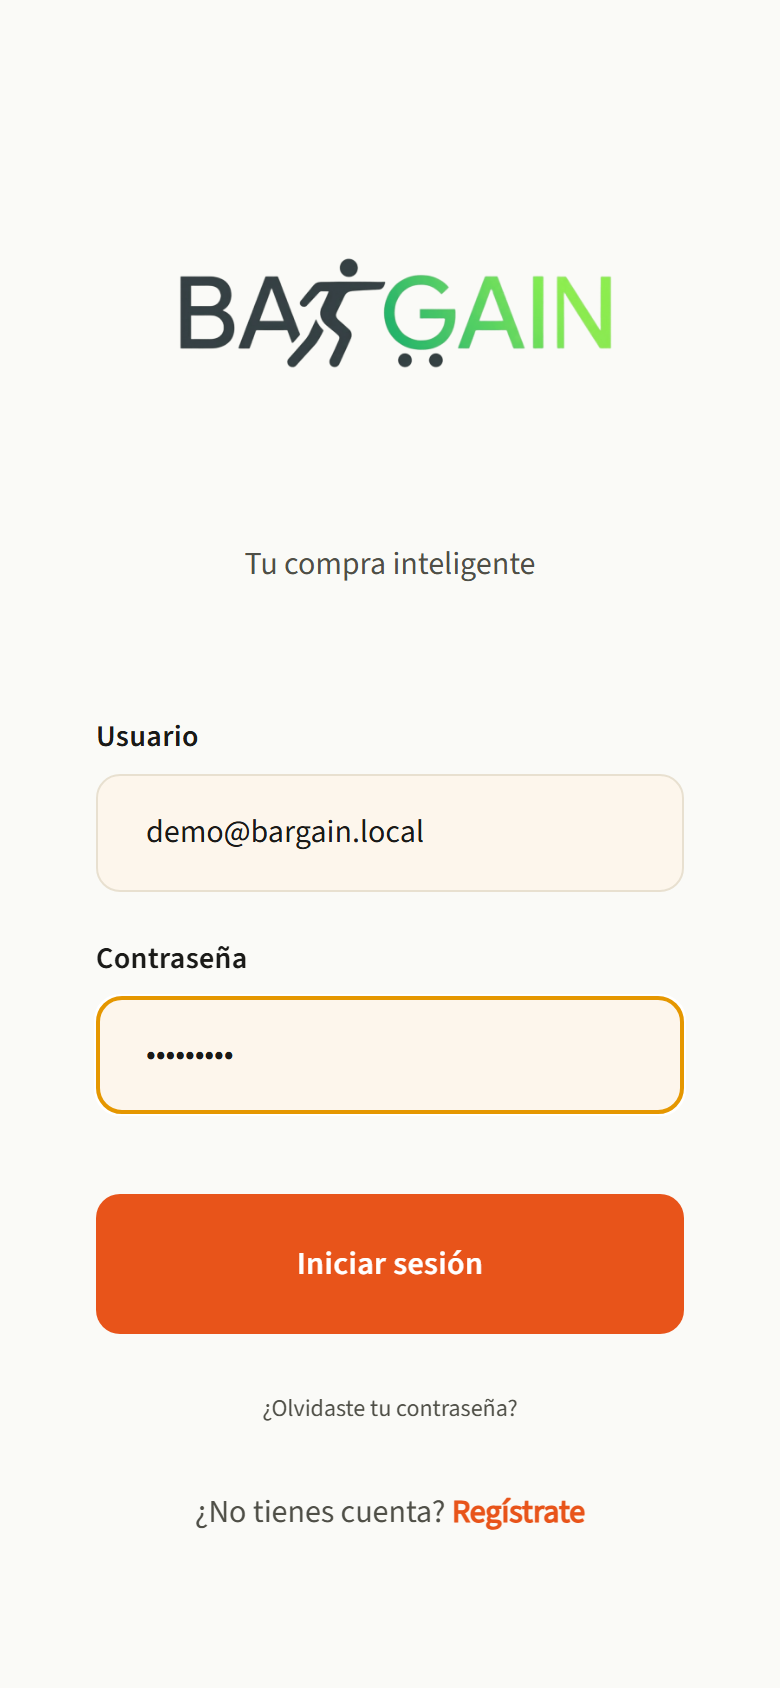
\includegraphics[width=0.32\textwidth]{diagramas/capturas/mobile-login.png}
\hfill
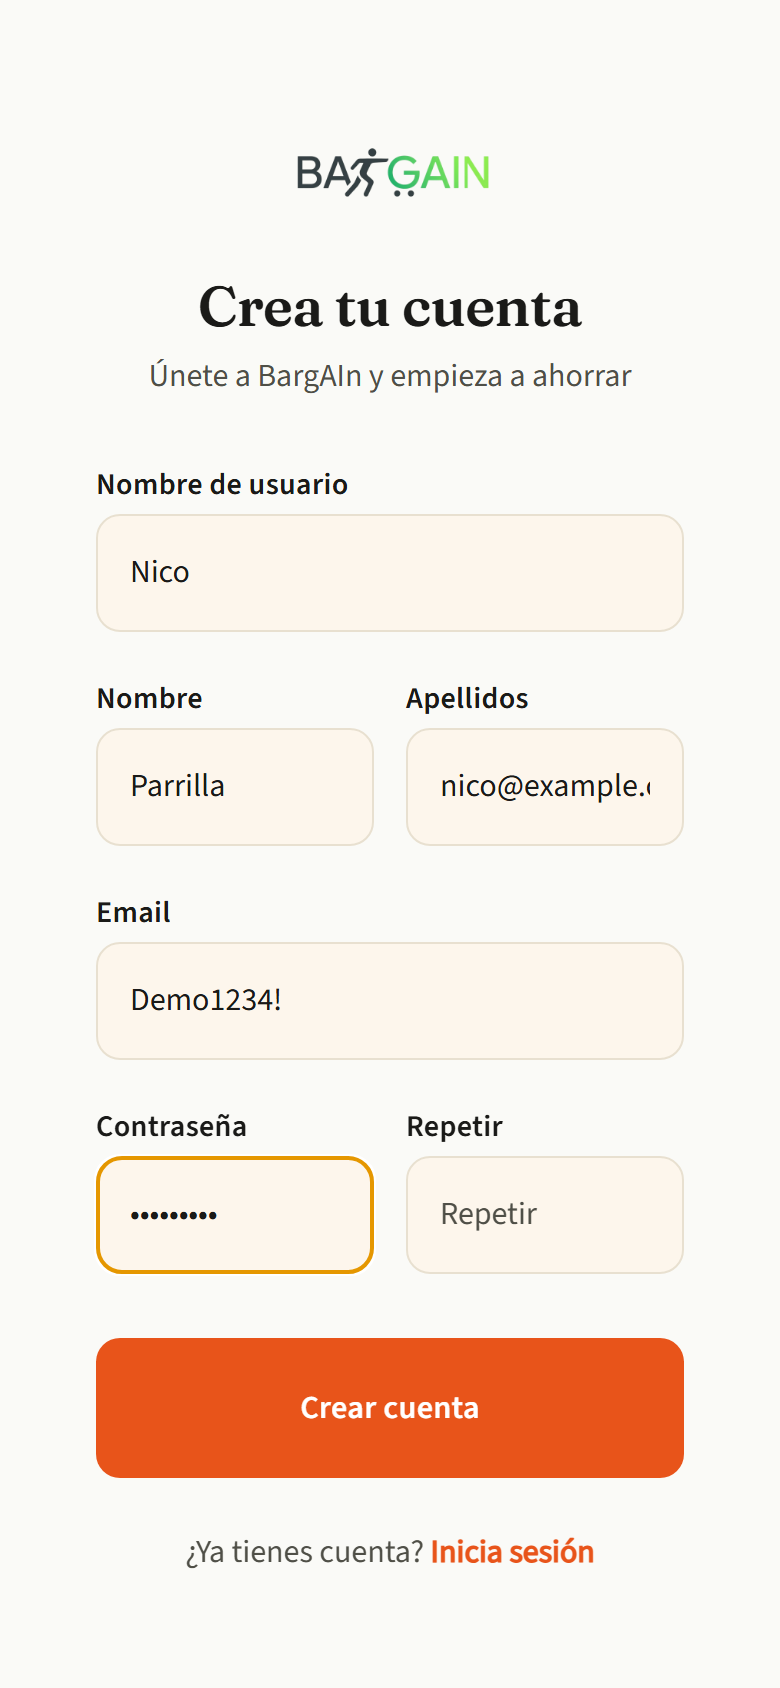
\includegraphics[width=0.32\textwidth]{diagramas/capturas/mobile-registro.png}
\caption{Pantallas de inicio de sesi\'on y registro}
\label{fig:ui-acceso}
\end{figure}

\section{Pantalla principal (Home)}\label{sec:manual-home}

La pantalla de inicio centraliza la informaci\'on m\'as relevante del usuario:

\begin{itemize}
  \item Resumen de listas activas con el precio estimado en la tienda m\'as barata cercana.
  \item CTA para crear lista cuando el usuario no tiene listas activas.
  \item Buscador global para navegar r\'apidamente a catálogo o funciones de compra.
  \item Acceso directo al asistente y a las alertas de precio activas.
\end{itemize}

\begin{figure}[htbp]
\centering
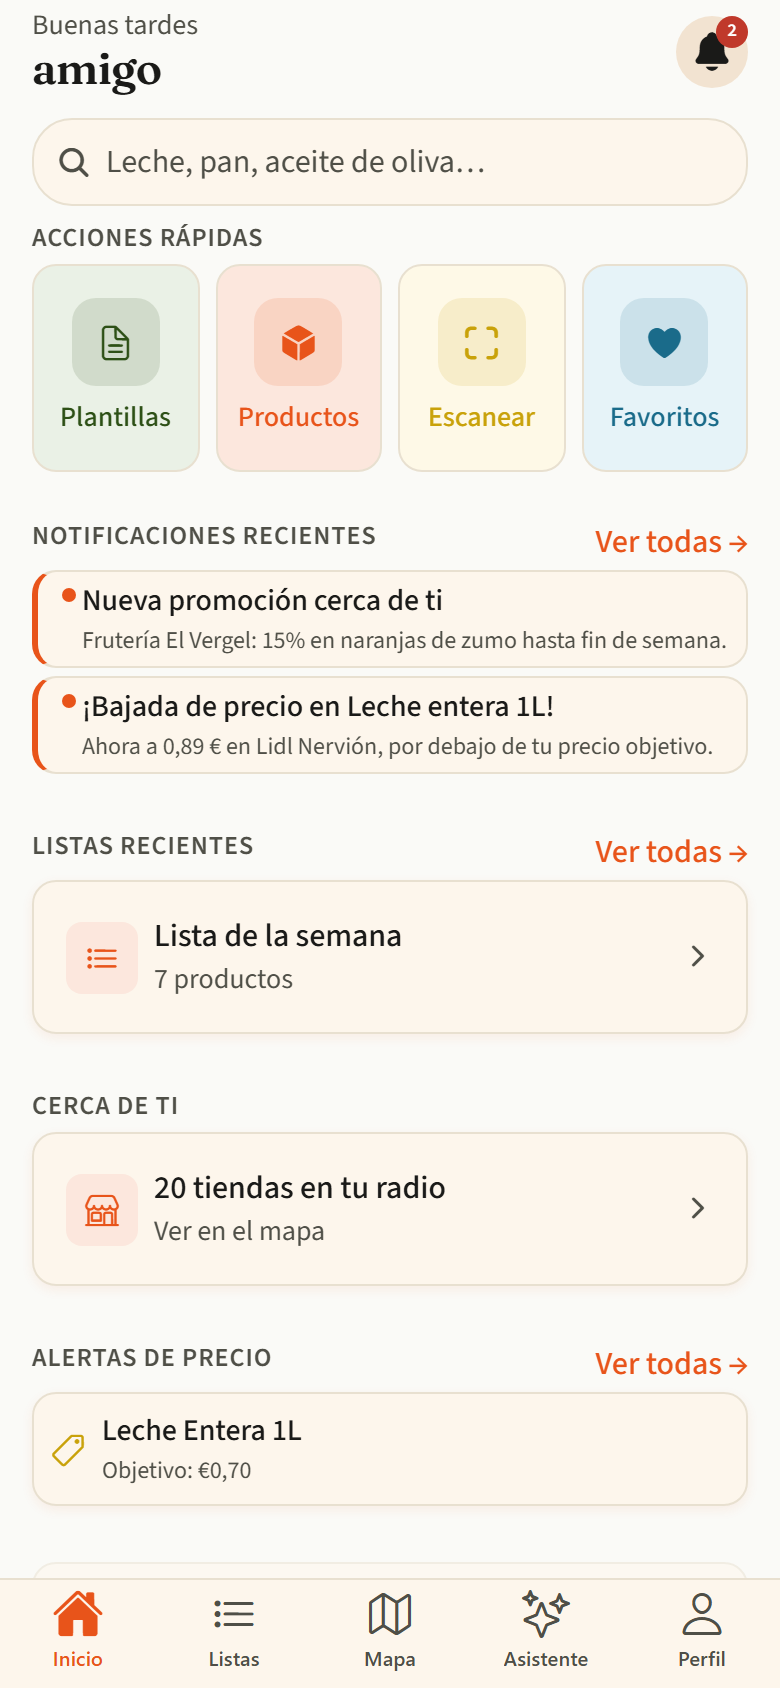
\includegraphics[width=0.40\textwidth]{diagramas/capturas/mobile-home.png}
\caption{Pantalla principal --- Dashboard}
\label{fig:ui-dashboard}
\end{figure}

\section{Gesti\'on de listas de compra}\label{sec:manual-listas}

\begin{enumerate}
  \item Crear lista con nombre personalizado (pesta\~na ``Mi Lista'' \textrightarrow{}
    bot\'on ``Nueva lista'').
  \item Abrir detalle de lista para ver \'items agrupados por categor\'ia.
  \item A\~nadir productos desde cat\'alogo o buscador con autocompletado.
  \item Ajustar cantidades con controles r\'apidos ``$+$/$-$''.
  \item Marcar productos como comprados (swipe-to-check) o eliminarlos (swipe-to-delete).
  \item Renombrar listas o convertirlas en plantilla para reutilizaci\'on futura.
  \item Compartir lista con colaboradores (hasta 10 usuarios por lista).
  \item Abrir ``Ruta optimizada'' para calcular, guardar y reutilizar la \'ultima ruta por lista.
\end{enumerate}

\begin{figure}[htbp]
\centering
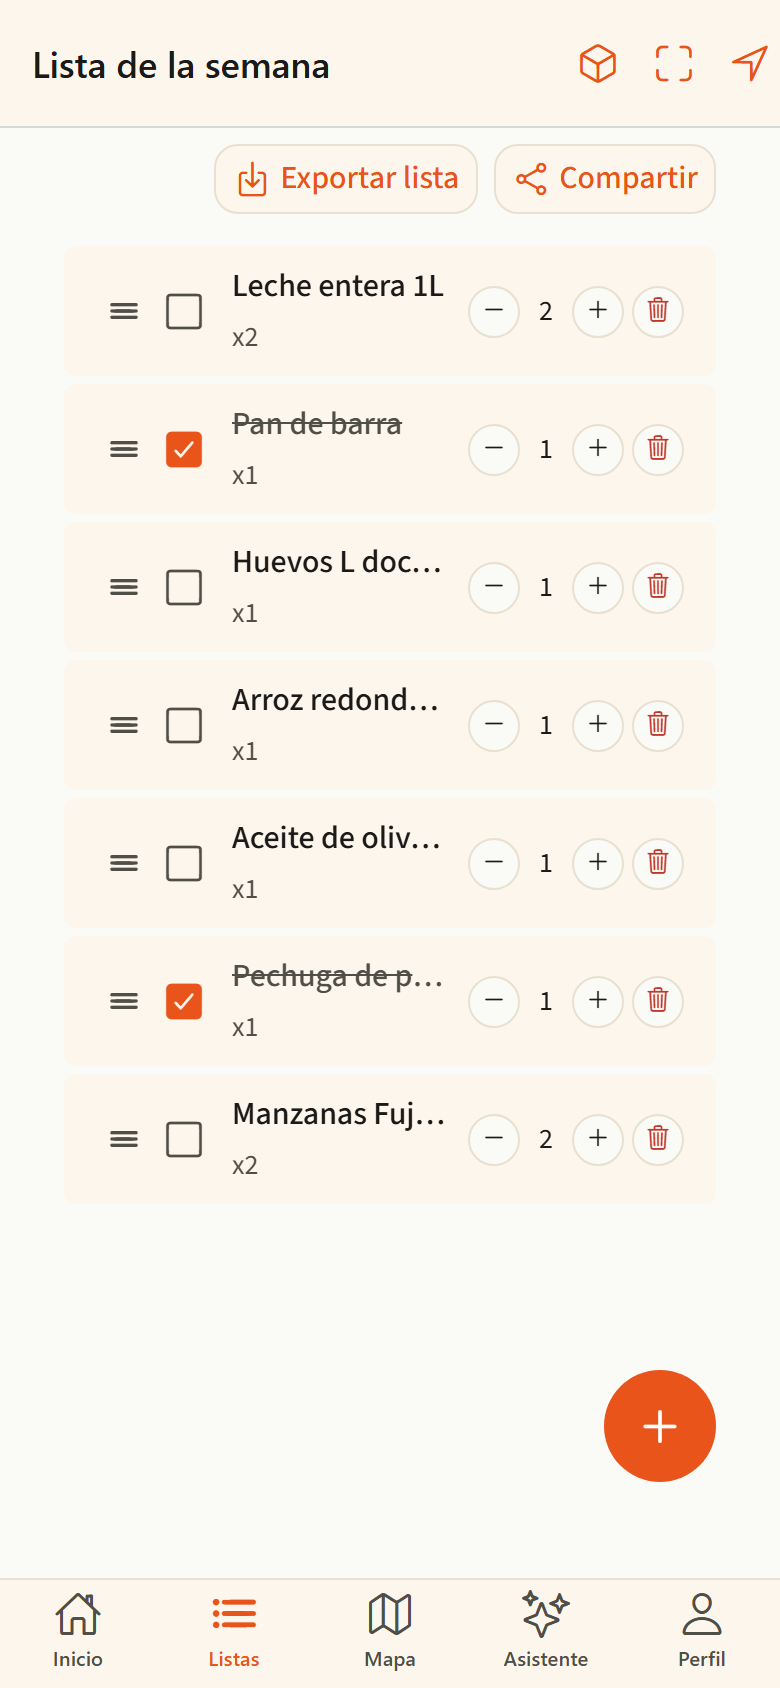
\includegraphics[width=0.40\textwidth]{diagramas/capturas/mobile-lista-detalle.png}
\caption{Pantalla de gesti\'on de lista de compra}
\label{fig:ui-lista}
\end{figure}

\section{Cat\'alogo y detalle de producto}\label{sec:manual-catalogo}

\begin{itemize}
  \item Cat\'alogo paginado con filtros plegables por categor\'ia, precio y distancia.
  \item Tarjetas de producto con precio m\'inimo detectado y nombre de la tienda m\'as barata.
  \item Acci\'on de a\~nadido r\'apido a lista desde la tarjeta (un tap).
  \item Detalle de producto con comparaci\'on de precios por tienda (tabla ordenable).
  \item Hist\'orico de precios con gr\'afico de evoluci\'on temporal.
\end{itemize}

\section{Mapa de tiendas}\label{sec:manual-mapa}

\begin{itemize}
  \item Visualizaci\'on de tiendas cercanas sobre mapa interactivo (React Native Maps).
  \item Marcadores diferenciados por cadena con badge de precio m\'inimo de la lista activa.
  \item Panel de tiendas plegable con detalles de la tienda seleccionada.
  \item Apertura de perfil de tienda desde el mapa y desde la lista de favoritas.
  \item Gesti\'on de tiendas favoritas (guardar, eliminar, acceder r\'apido).
\end{itemize}

\section{Alertas y notificaciones}\label{sec:manual-notificaciones}

\begin{itemize}
  \item Creaci\'on de alertas de precio: al abrir el detalle de un producto, pulsar ``Crear
    alerta'' e introducir el precio objetivo.
  \item Edici\'on y eliminaci\'on de alertas existentes desde la pantalla ``Mis alertas''.
  \item Bandeja de notificaciones con marcado como le\'ido individual o masivo y borrado
    funcional (soft-delete).
  \item Notificaciones push en el dispositivo para alertas de precio, nuevas promociones y
    cambios en listas compartidas.
\end{itemize}

\section{Perfil y preferencias}\label{sec:manual-perfil}

El usuario puede desde la pesta\~na ``Perfil'':

\begin{itemize}
  \item Editar datos b\'asicos (nombre, foto de avatar, tel\'efono).
  \item Ajustar preferencias del optimizador: radio de b\'usqueda (1--20 km), pesos
    $w_{precio}$/$w_{distancia}$/$w_{tiempo}$ (sliders que suman 1.0) y modo de
    optimizaci\'on (precio / distancia / balanced).
  \item Configurar preferencias de notificaciones (push, email, tipos de alerta).
  \item Cerrar sesi\'on (invalida el refresh token).
\end{itemize}

\section{Ruta optimizada persistente y rec\'alculo}\label{sec:manual-ruta}

Flujo recomendado:

\begin{enumerate}
  \item Entrar en una lista y pulsar ``Ruta optimizada''.
  \item Si existe una ruta previa para esa lista, se carga autom\'aticamente desde base de datos.
  \item Revisar paradas, productos por parada y precio total estimado.
  \item Pulsar ``Recalcular ruta'' para lanzar una nueva optimizaci\'on con ubicaci\'on y pesos
    actuales.
  \item Pulsar ``Ver en mapa'' para abrir la ruta circular en la app de mapas del dispositivo.
\end{enumerate}

Comportamiento persistente: la app no pierde la ruta al salir de la pantalla. Al volver, recupera
la \'ultima optimizaci\'on guardada de esa lista.

\begin{figure}[htbp]
\centering
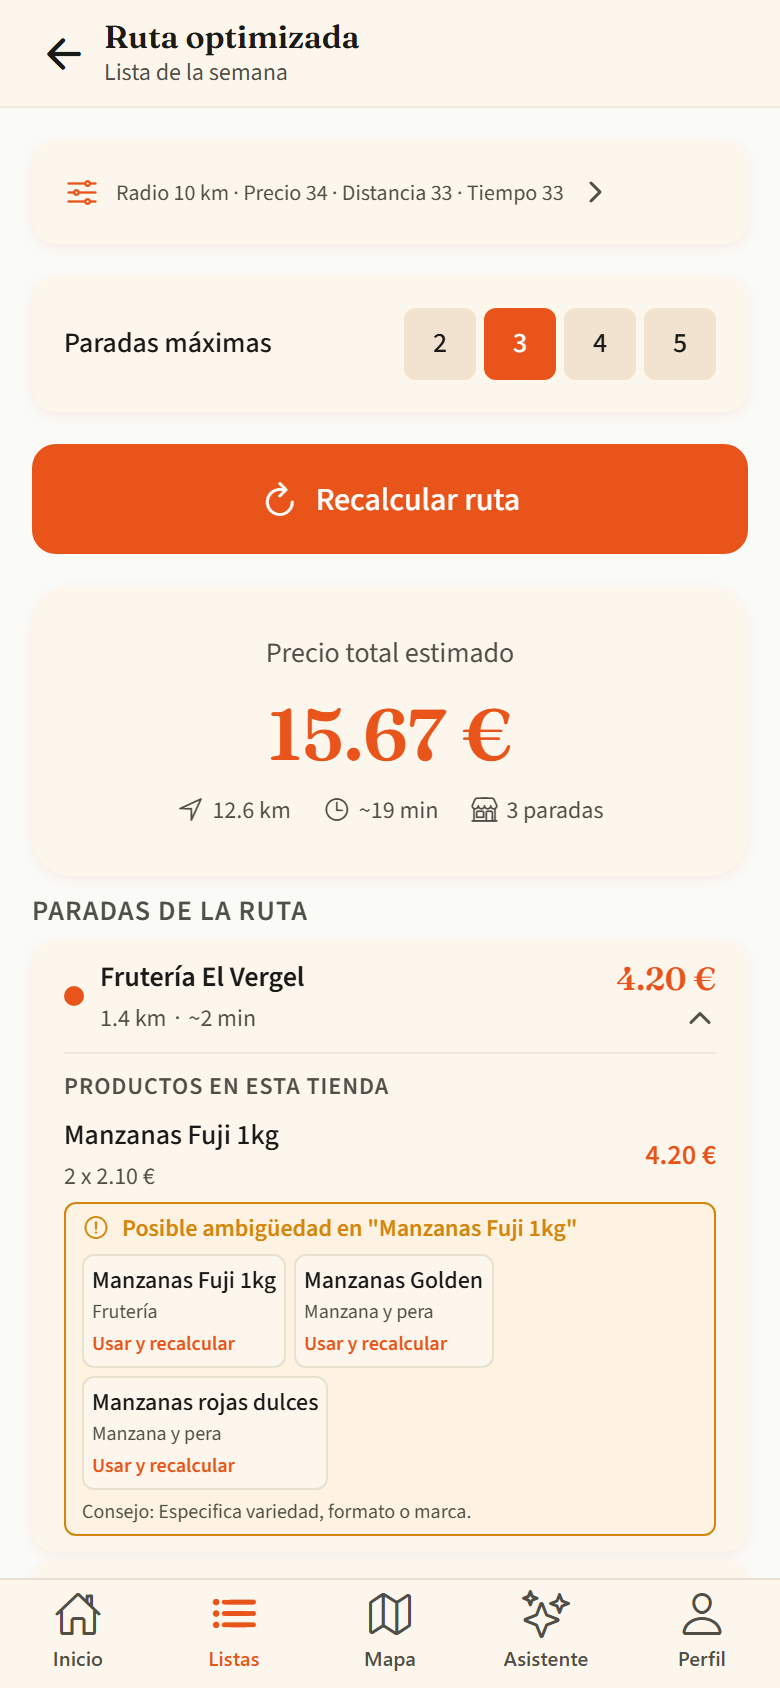
\includegraphics[width=0.40\textwidth]{diagramas/capturas/mobile-ruta.png}
\caption{Pantalla del optimizador con comparativa de rutas}
\label{fig:ui-optimizador}
\end{figure}

\section{M\'odulo OCR: captura de ticket}\label{sec:manual-ocr}

El flujo de captura de lista por c\'amara sigue un wizard de tres pasos:

\begin{enumerate}
  \item \textbf{Captura:} Acceder desde ``Mi Lista'' \textrightarrow{} icono de c\'amara.
    Apuntar la c\'amara al ticket o lista escrita. Se puede usar la galer\'ia como alternativa.
  \item \textbf{Revisi\'on:} La app muestra los productos reconocidos con nivel de confianza
    (chip de color: verde $\geq$ 80\%, amarillo 50--79\%, rojo $<$ 50\%).
    El usuario puede corregir el texto de cualquier \'item inline o eliminar los no deseados.
  \item \textbf{Confirmaci\'on:} Seleccionar la lista destino (existente o nueva) y confirmar
    para a\~nadir todos los \'items reconocidos.
\end{enumerate}

\begin{figure}[htbp]
\centering
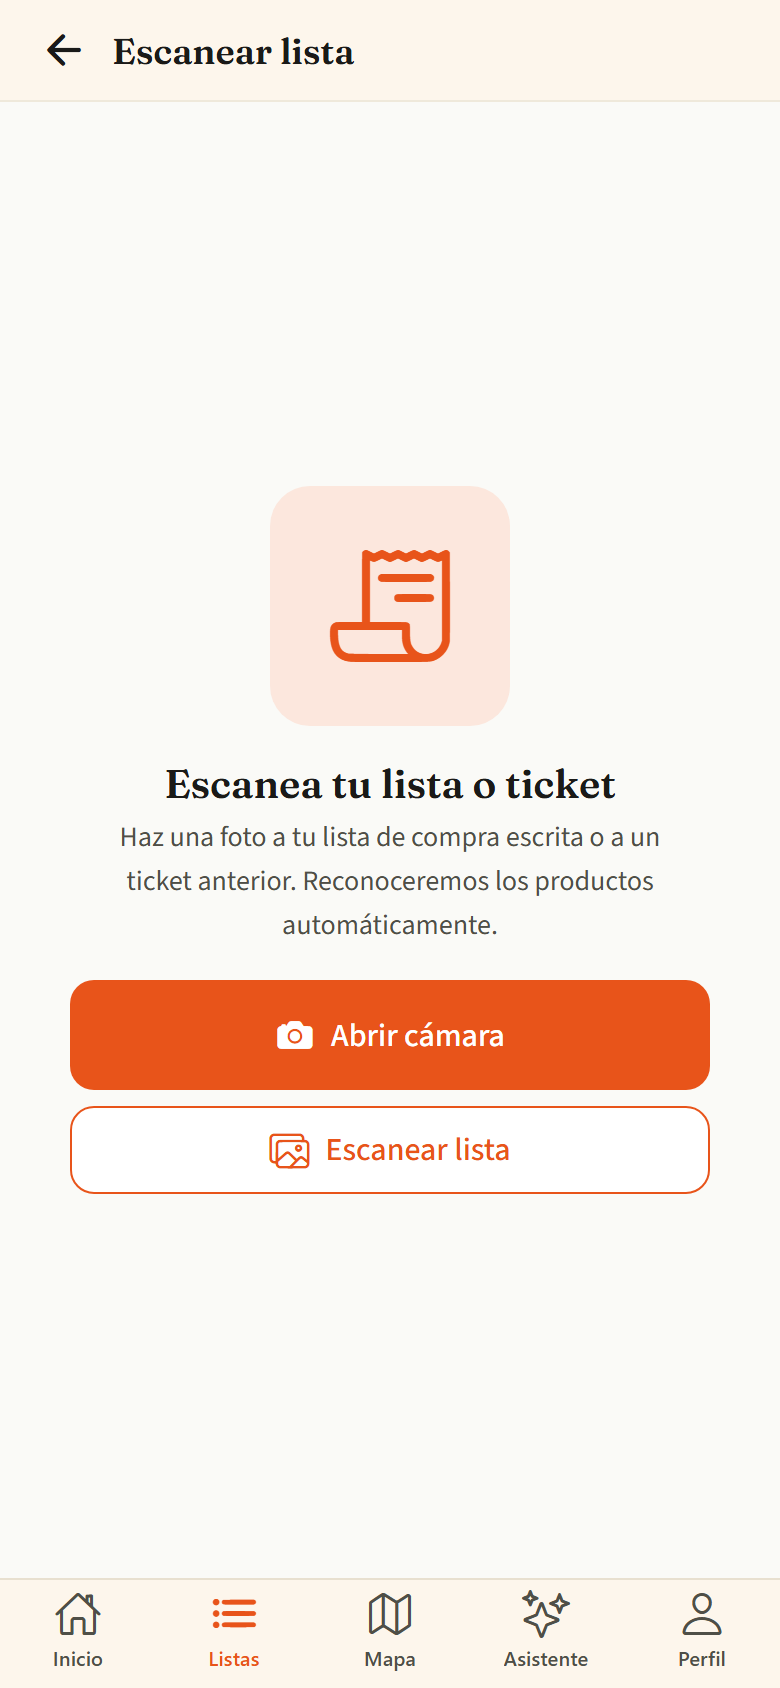
\includegraphics[width=0.32\textwidth]{diagramas/capturas/mobile-ocr-captura.png}
\hfill
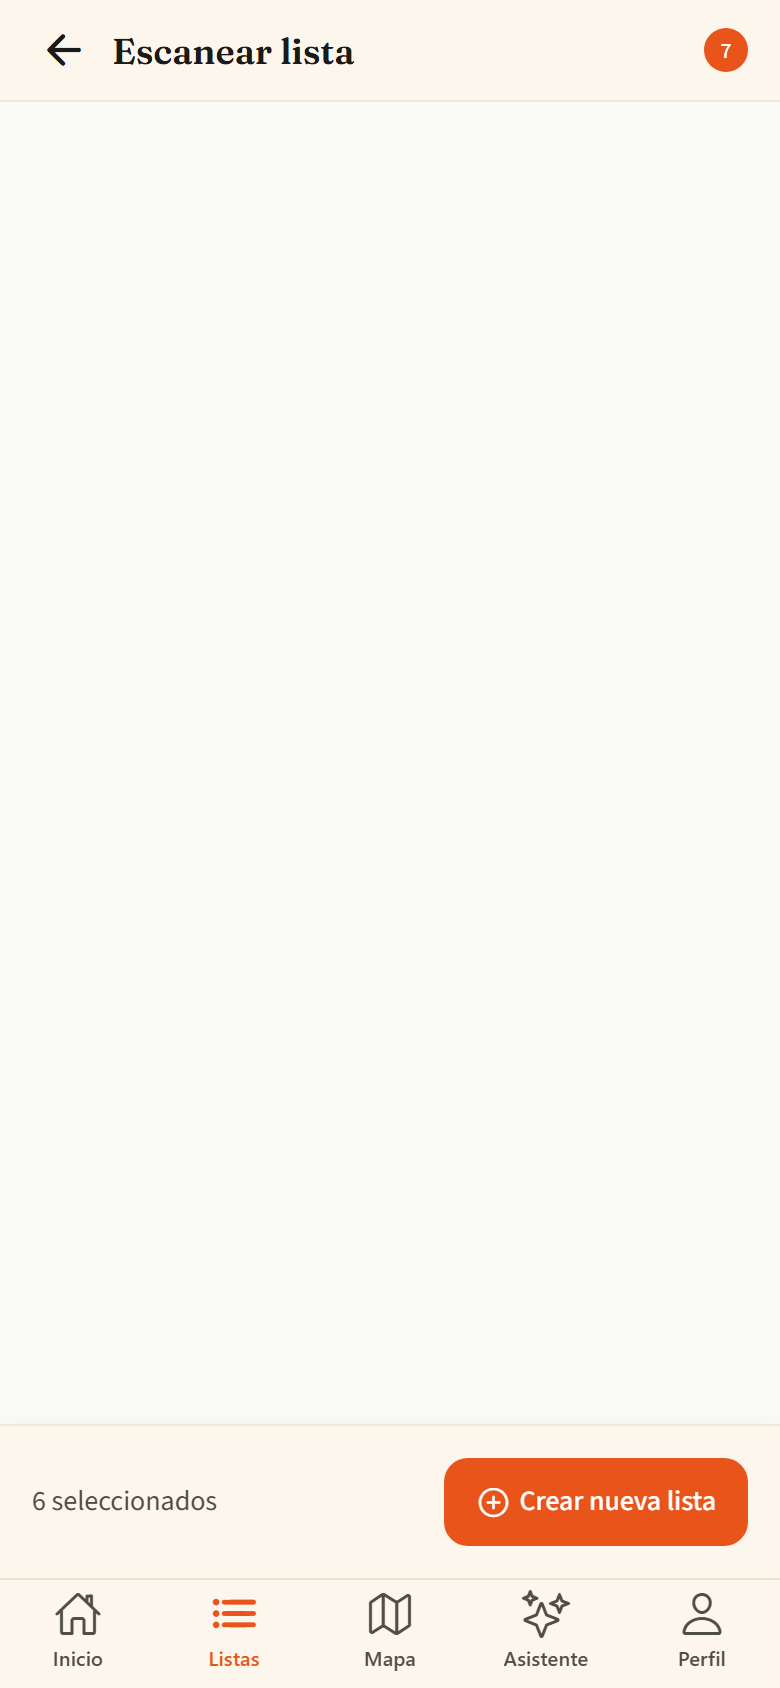
\includegraphics[width=0.32\textwidth]{diagramas/capturas/mobile-ocr-revision.png}
\caption{Flujo OCR: captura de ticket (izquierda) y revisi\'on de \'items (derecha)}
\label{fig:ui-ocr}
\end{figure}

\section{Asistente LLM}\label{sec:manual-asistente}

La pantalla del asistente sigue el patr\'on de chat est\'andar:

\begin{itemize}
  \item Mensajes del usuario alineados a la derecha (burbuja verde).
  \item Respuestas del asistente alineadas a la izquierda (burbuja gris).
  \item Las respuestas con productos, precios o tiendas incluyen chips interactivos para a\~nadir
    el producto a la lista activa directamente desde el chat.
  \item El asistente s\'olo responde preguntas relacionadas con la compra dom\'estica. Si se hace
    una pregunta fuera de ese \'ambito, responde educadamente indicando su alcance.
\end{itemize}

\begin{figure}[htbp]
\centering
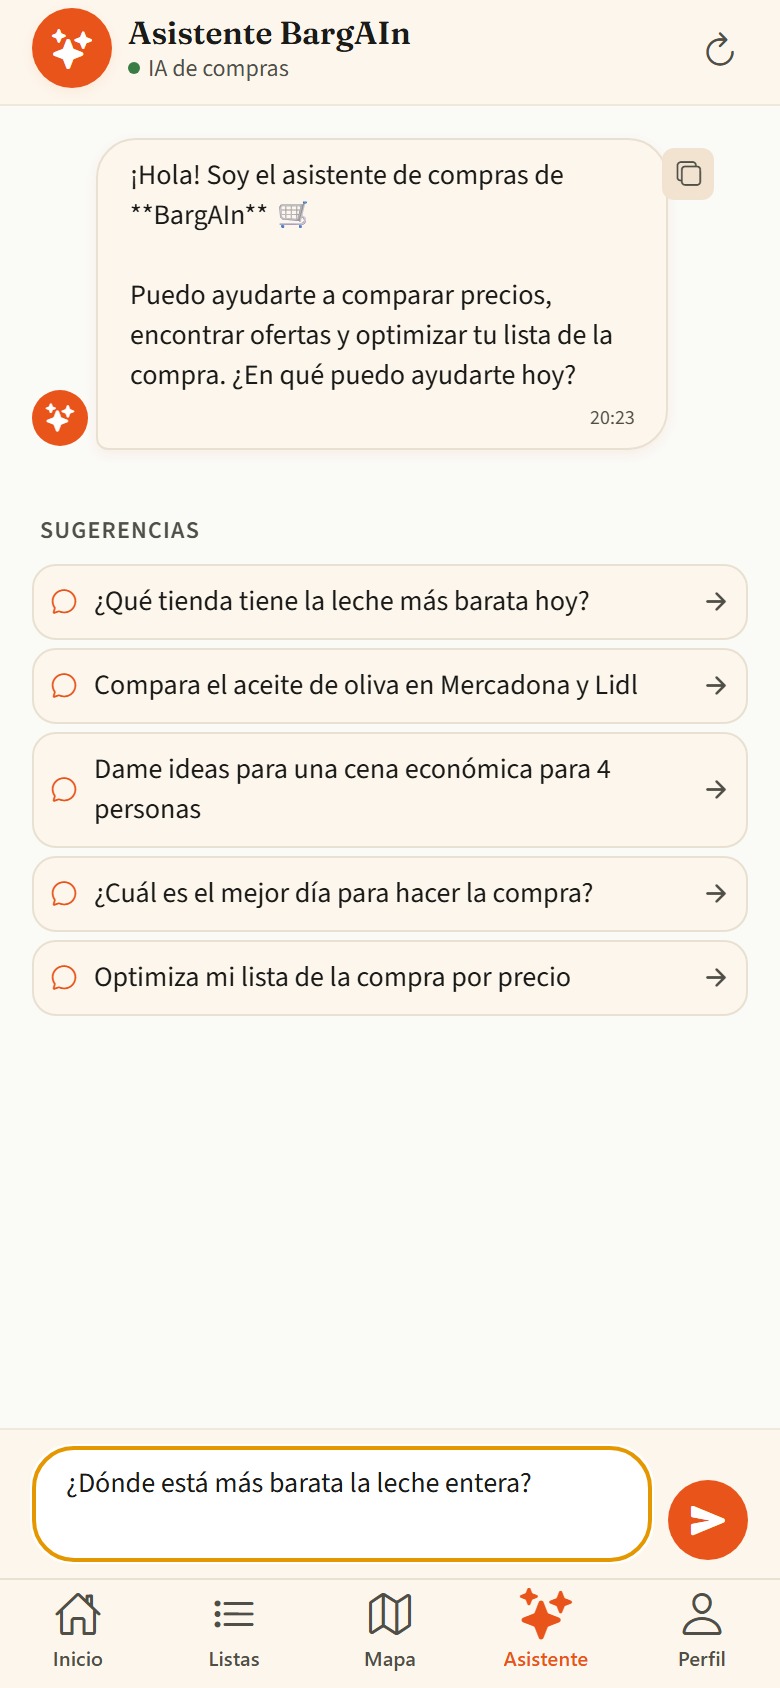
\includegraphics[width=0.40\textwidth]{diagramas/capturas/mobile-asistente.png}
\caption{Pantalla del asistente conversacional LLM}
\label{fig:ui-asistente}
\end{figure}

\section{Checklist en bloqueo de iPhone}\label{sec:manual-lockscreen}

Desde la pantalla de ruta optimizada, el bot\'on ``Checklist en bloqueo'' publica una notificaci\'on
interactiva con las acciones de marcar cada producto como comprado. Al pulsar una acci\'on en
pantalla bloqueada, el \'item se marca como comprado y la notificaci\'on se actualiza.

\section{Portal Business (web)}\label{sec:manual-business}

Para cuentas PYME, el portal web (\texttt{/business}) ofrece:

\begin{enumerate}
  \item \textbf{Registro:} Formulario de onboarding con datos del negocio (nombre, CIF, direcci\'on,
    web). La cuenta queda en estado ``pendiente'' hasta que un administrador la aprueba.
  \item \textbf{Gesti\'on de precios:} Tabla editable con todos los productos del negocio y sus
    precios actuales. Actualizaci\'on individual o mediante carga masiva en CSV.
  \item \textbf{Gesti\'on de promociones:} Crear, activar y desactivar promociones con descuento
    fijo o porcentual, fecha de fin y cantidad m\'inima.
  \item \textbf{Perfil de negocio:} Editar descripci\'on, horario, tel\'efono, imagen.
  \item \textbf{Estad\'isticas:} N\'umero de visualizaciones del perfil y comparativa de precios
    con competidores del entorno (alerta autom\'atica cuando la diferencia supera el umbral
    configurado).
\end{enumerate}

\section{Uso desde el navegador web}\label{sec:manual-web}

Adem\'as del portal PYME, la aplicaci\'on de usuario final puede ejecutarse en un navegador de
escritorio reutilizando la misma app Expo. La interfaz se adapta autom\'aticamente al ancho de la
ventana y habilita conveniencias propias del escritorio (Fase 13):

\begin{itemize}
  \item \textbf{Dise\~no adaptable:} el contenido se centra a un ancho legible y los cat\'alogos y
    listados muestran varias columnas (2--4) en pantallas anchas. En el mapa, el panel de tiendas
    se ancla a la derecha en lugar de mostrarse debajo.
  \item \textbf{Rat\'on y teclado:} atajo \texttt{Cmd/Ctrl+K} para enfocar el buscador,
    \texttt{Enter} para a\~nadir un producto a la lista y \texttt{Esc} para cerrar di\'alogos, con
    realces \emph{hover} sobre tarjetas y botones. El campo del asistente recibe el foco
    autom\'aticamente al abrir la pantalla.
  \item \textbf{Reordenar listas:} en el detalle de una lista se pueden arrastrar los \'items para
    reordenarlos (\emph{drag-and-drop}); el nuevo orden es v\'alido durante la sesi\'on.
  \item \textbf{Exportar y compartir:} botones para exportar la lista (\texttt{.txt}), la
    comparativa de precios (\texttt{.csv}) y la ruta, copiar la direcci\'on de una tienda al
    portapapeles y compartir el enlace directo a una lista o tienda.
  \item \textbf{Enlaces directos:} cada pantalla relevante tiene una URL propia, por lo que se
    puede compartir o guardar como marcador el estado actual (por ejemplo, una b\'usqueda concreta
    del cat\'alogo mediante \texttt{?q=}).
\end{itemize}

\section{Galer\'ia de capturas de la aplicaci\'on}\label{sec:manual-galeria}

Esta secci\'on recoge capturas reales de cada pantalla y funcionalidad de la aplicaci\'on
desplegada, agrupadas por contexto de uso: aplicaci\'on m\'ovil de usuario (viewport
390$\times$844), aplicaci\'on web de usuario (escritorio, 1440$\times$900) y portal web para
PYMEs. Todas las im\'agenes residen en \texttt{diagramas/capturas/}.

\subsection{Aplicaci\'on m\'ovil (usuario)}\label{subsec:galeria-movil}

\begin{figure}[htbp]
\centering
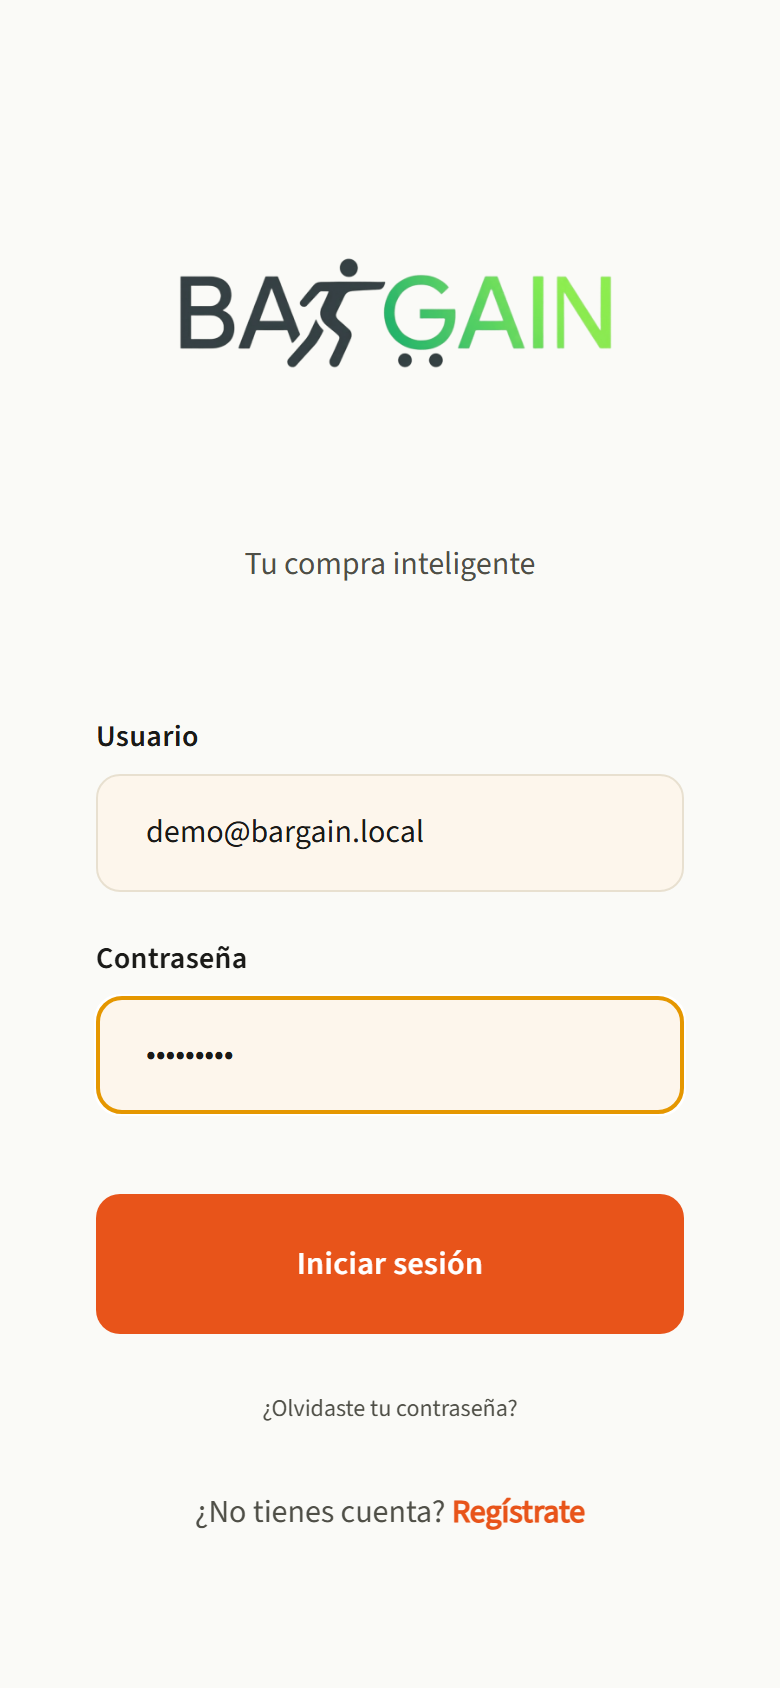
\includegraphics[width=0.30\textwidth]{diagramas/capturas/mobile-login.png}
\hfill
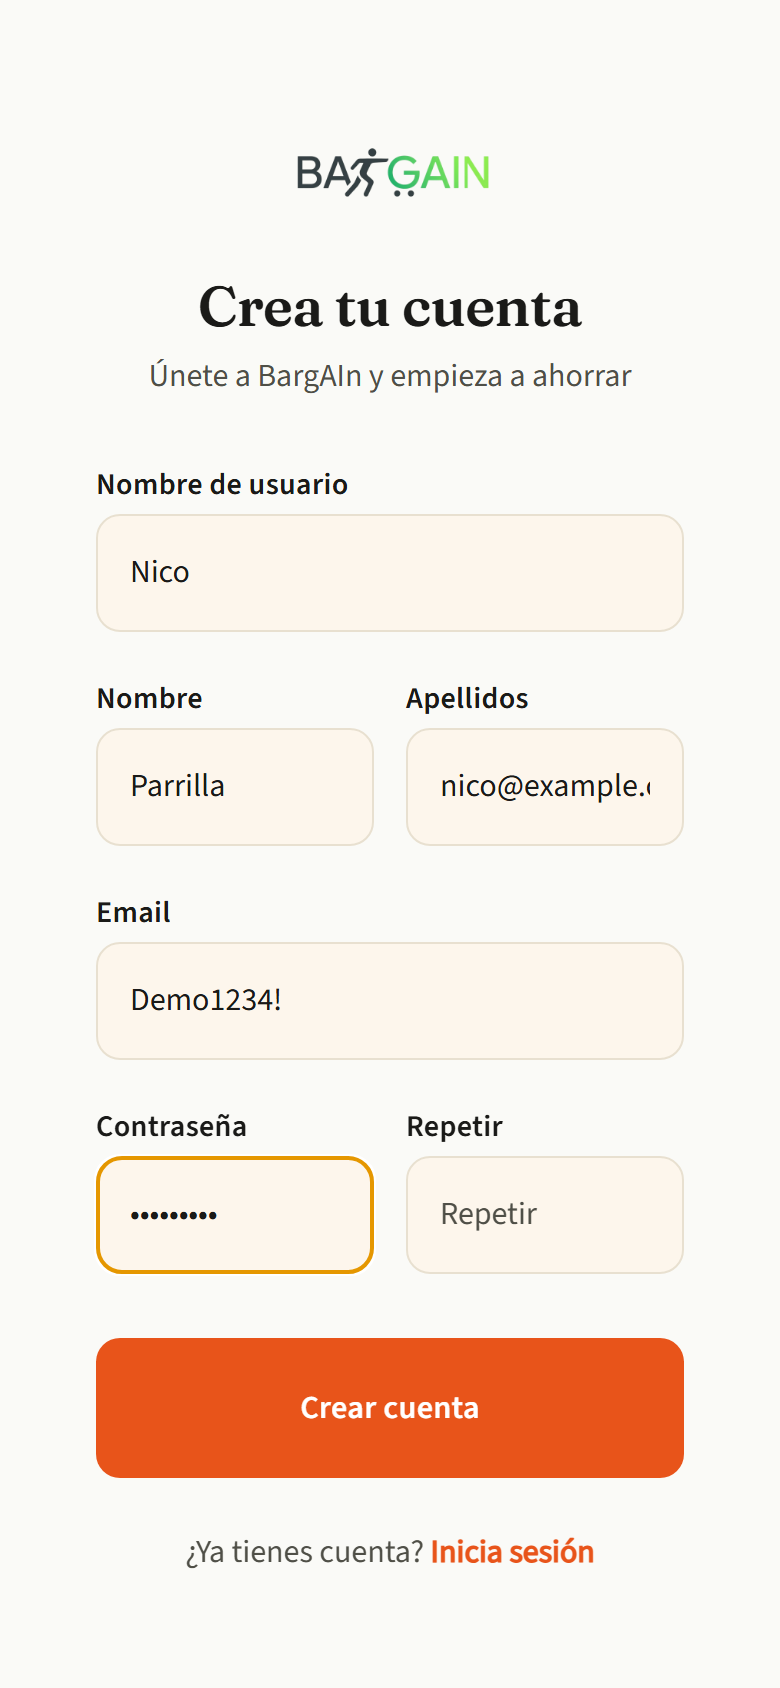
\includegraphics[width=0.30\textwidth]{diagramas/capturas/mobile-registro.png}
\caption{M\'ovil --- Inicio de sesi\'on (izquierda) y registro (derecha)}
\label{fig:cap-mobile-acceso}
\end{figure}

\begin{figure}[htbp]
\centering
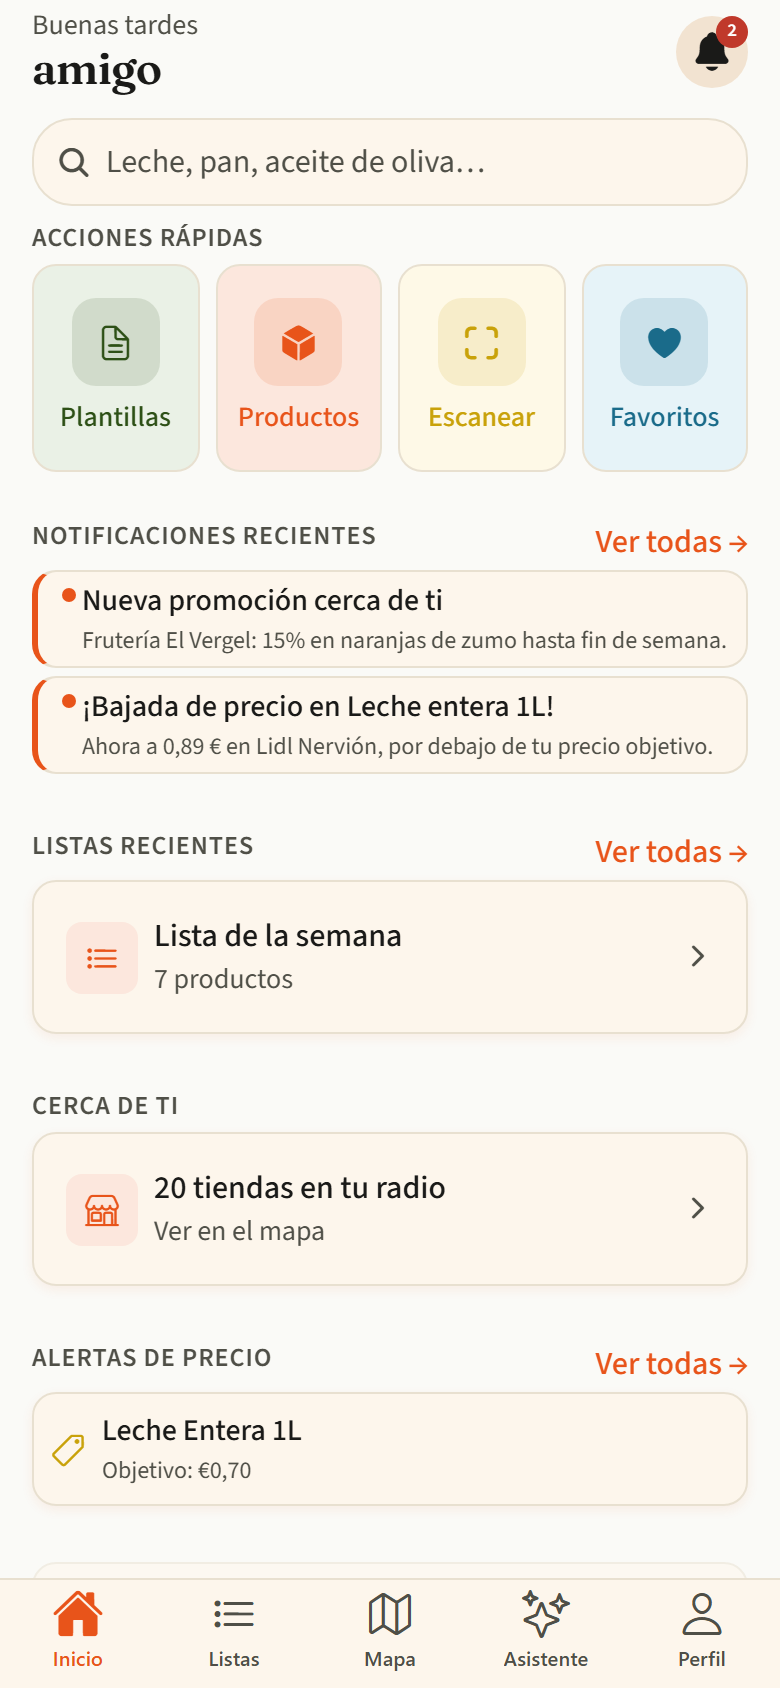
\includegraphics[width=0.30\textwidth]{diagramas/capturas/mobile-home.png}
\hfill
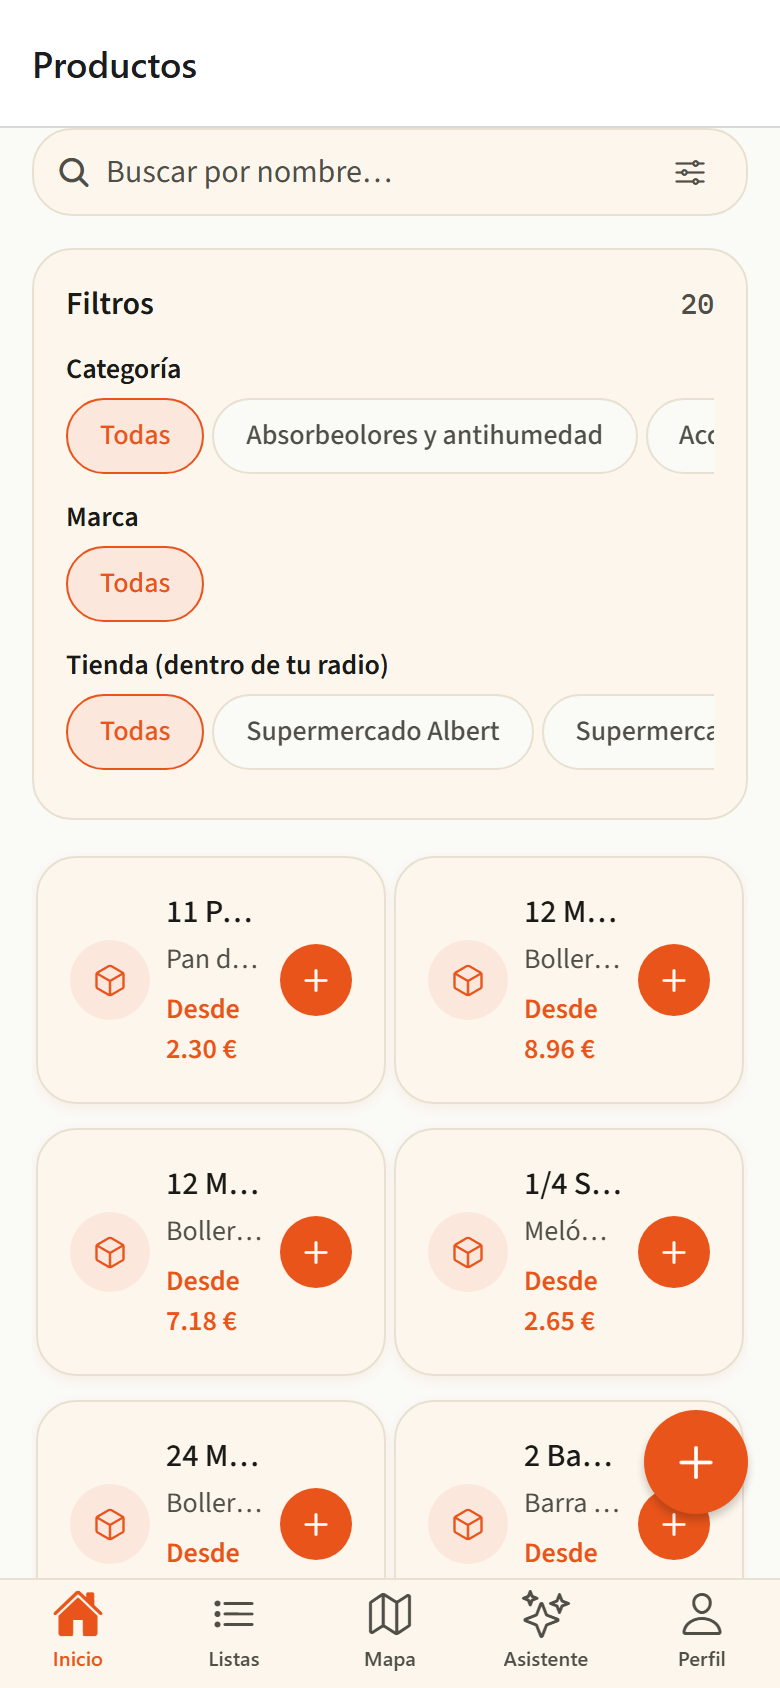
\includegraphics[width=0.30\textwidth]{diagramas/capturas/mobile-catalogo.png}
\caption{M\'ovil --- Pantalla principal (izquierda) y cat\'alogo de productos (derecha)}
\label{fig:cap-mobile-home-catalogo}
\end{figure}

\begin{figure}[htbp]
\centering
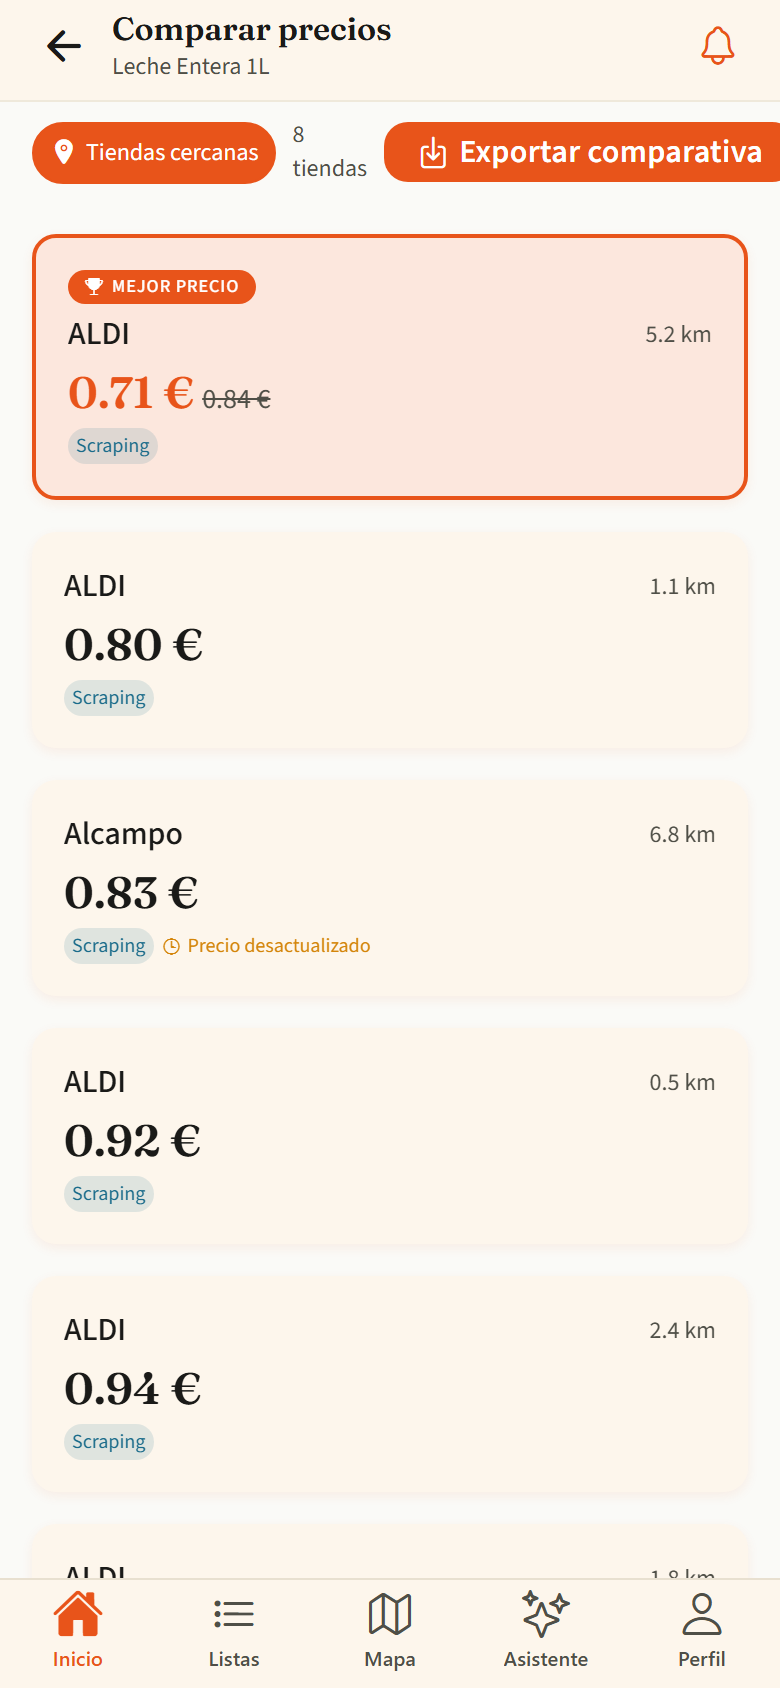
\includegraphics[width=0.30\textwidth]{diagramas/capturas/mobile-detalle-precio.png}
\hfill
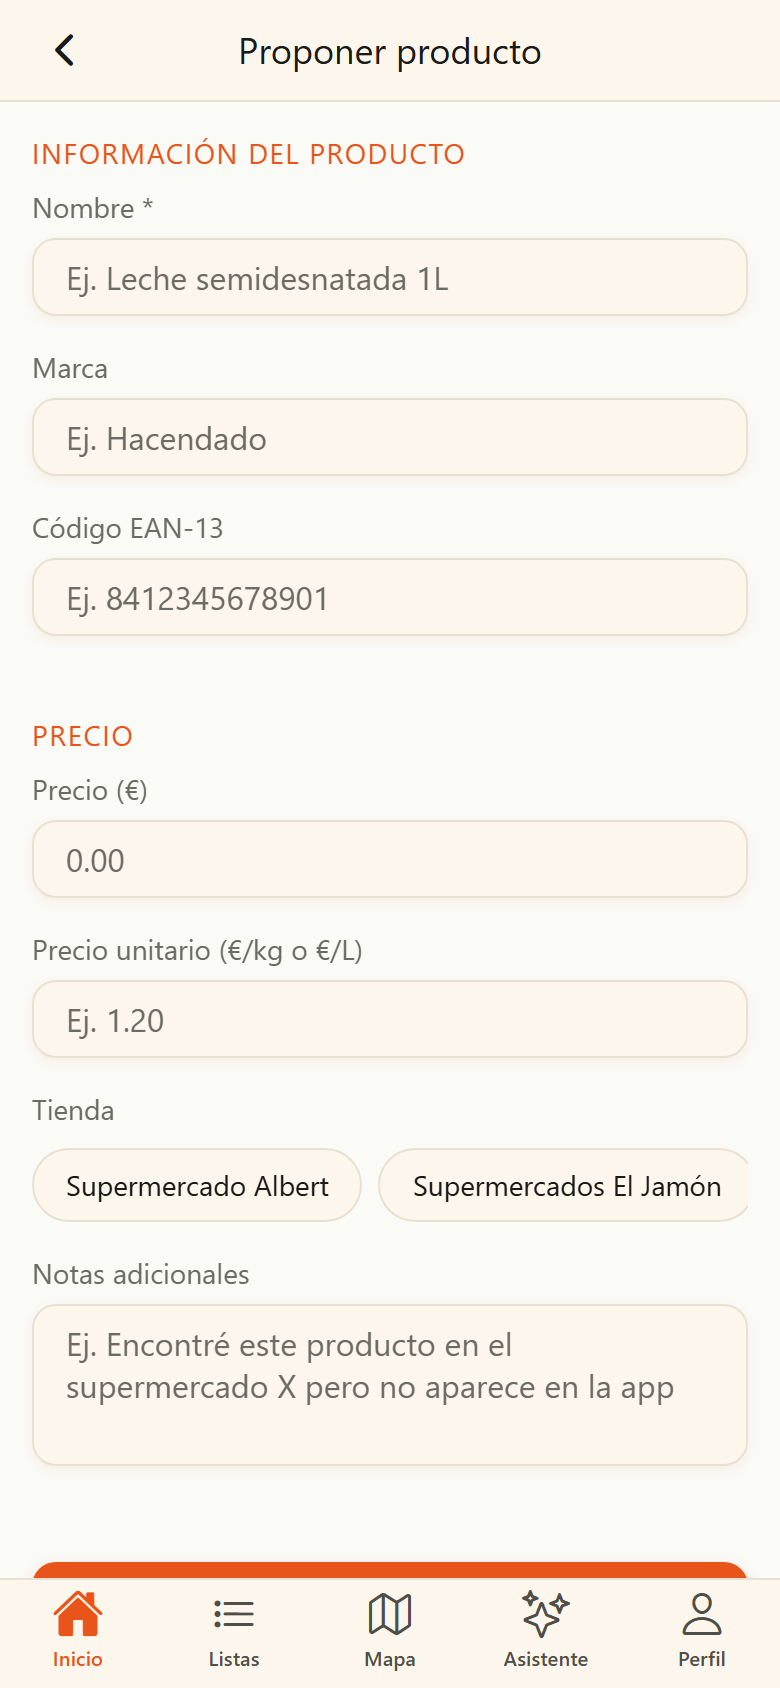
\includegraphics[width=0.30\textwidth]{diagramas/capturas/mobile-proponer.png}
\caption{M\'ovil --- Comparativa de precios por tienda (izquierda) y propuesta de producto (derecha)}
\label{fig:cap-mobile-precio-proponer}
\end{figure}

\begin{figure}[htbp]
\centering
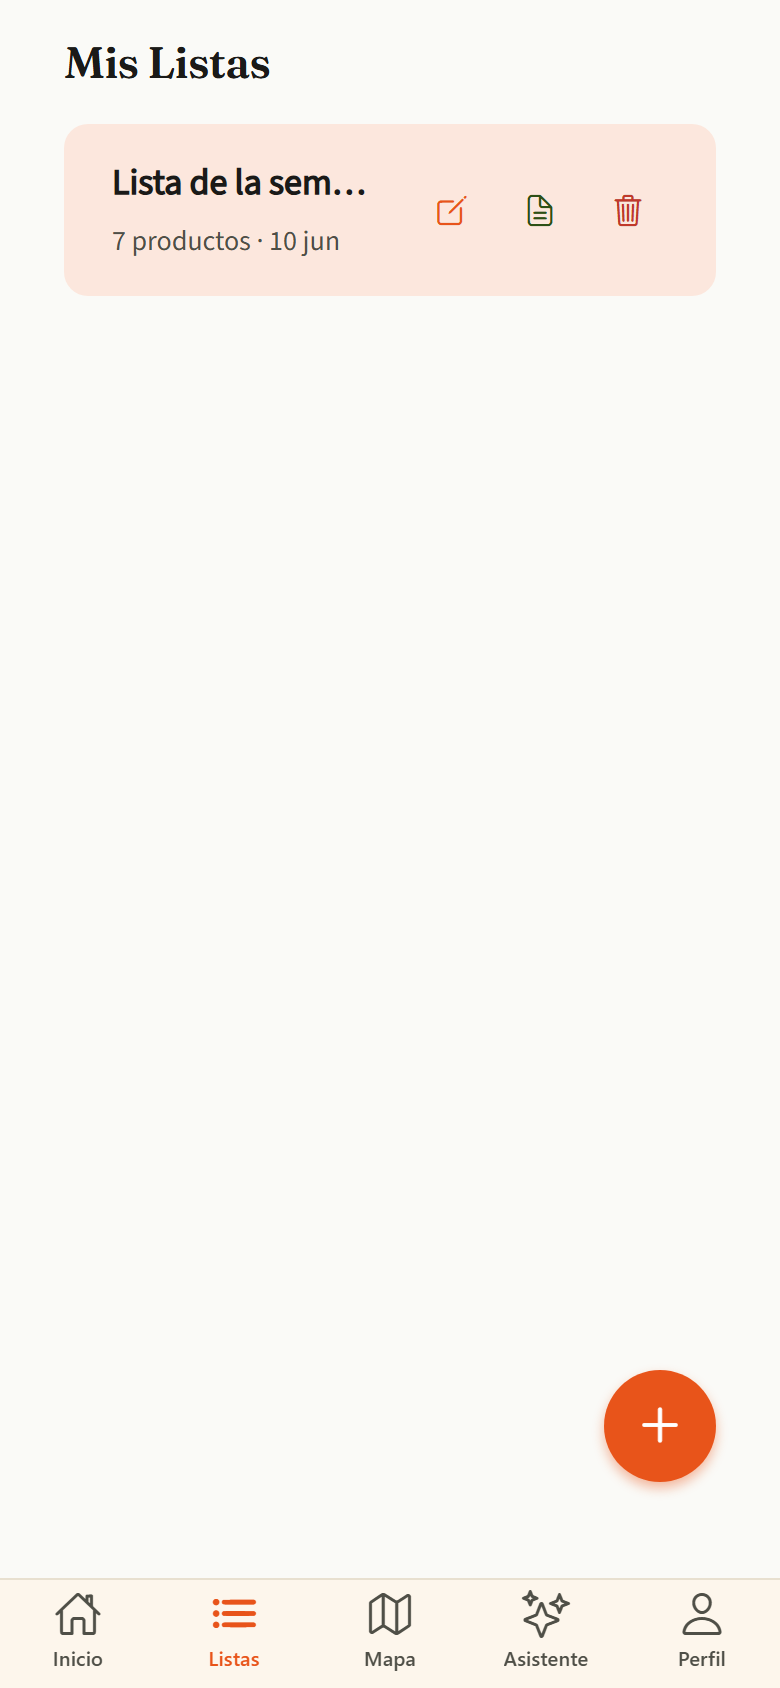
\includegraphics[width=0.30\textwidth]{diagramas/capturas/mobile-listas.png}
\hfill
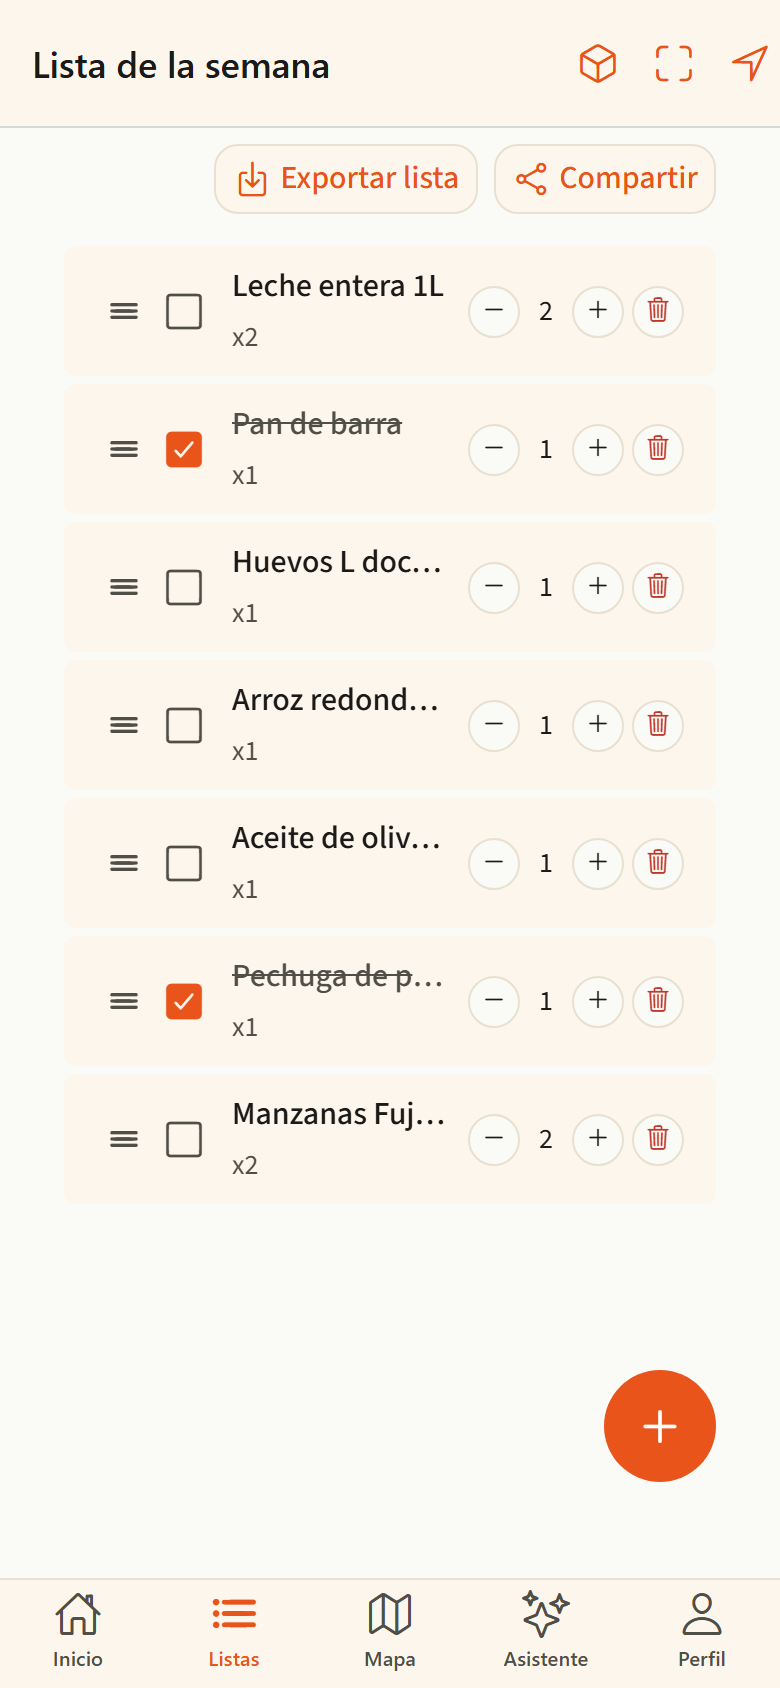
\includegraphics[width=0.30\textwidth]{diagramas/capturas/mobile-lista-detalle.png}
\caption{M\'ovil --- Listas de la compra (izquierda) y detalle de una lista (derecha)}
\label{fig:cap-mobile-listas}
\end{figure}

\clearpage

\begin{figure}[htbp]
\centering
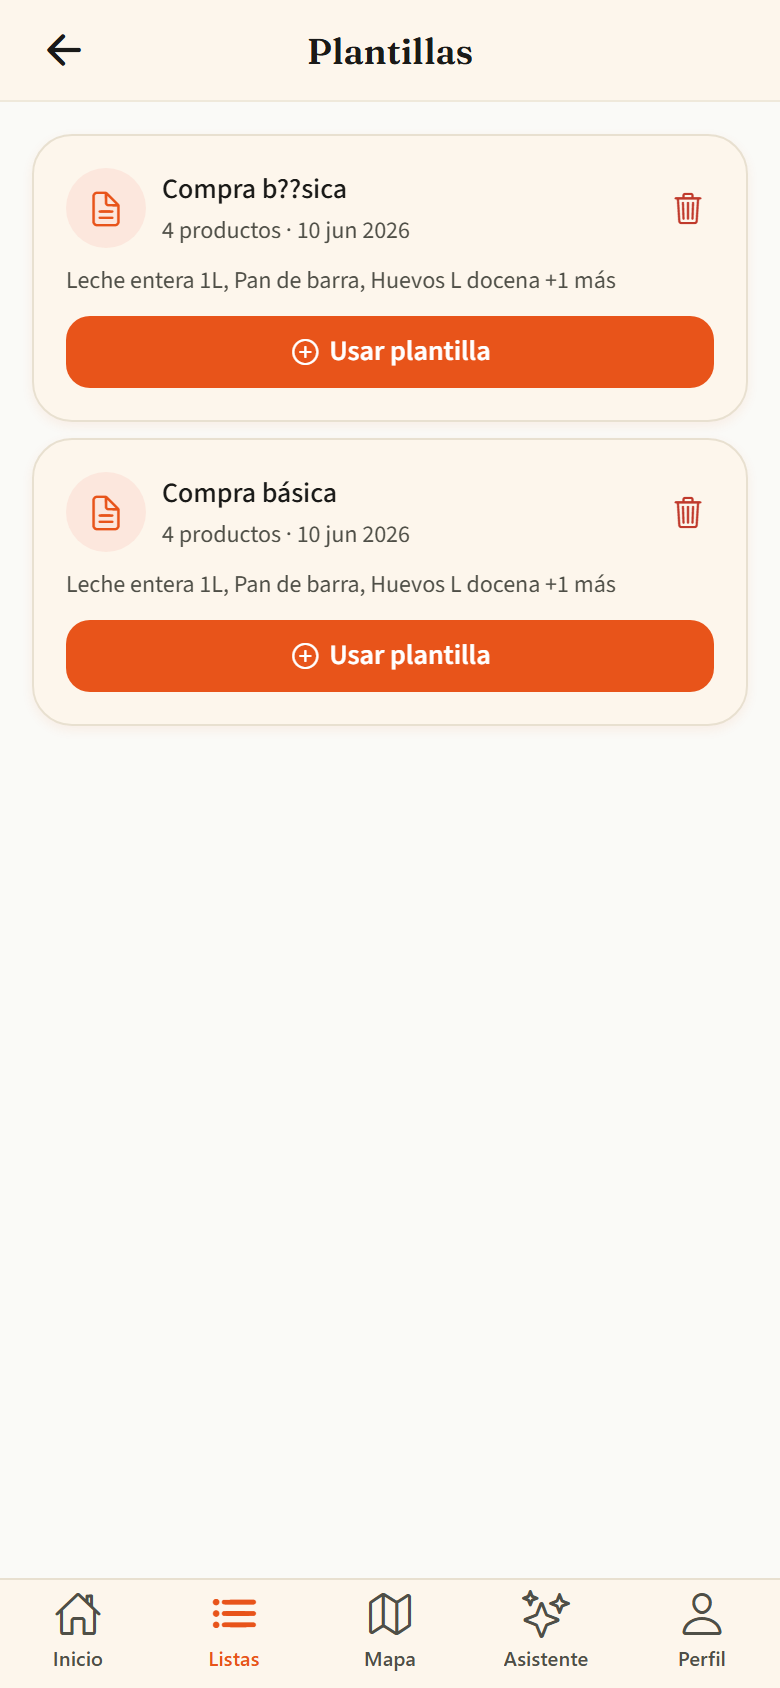
\includegraphics[width=0.30\textwidth]{diagramas/capturas/mobile-plantillas.png}
\hfill
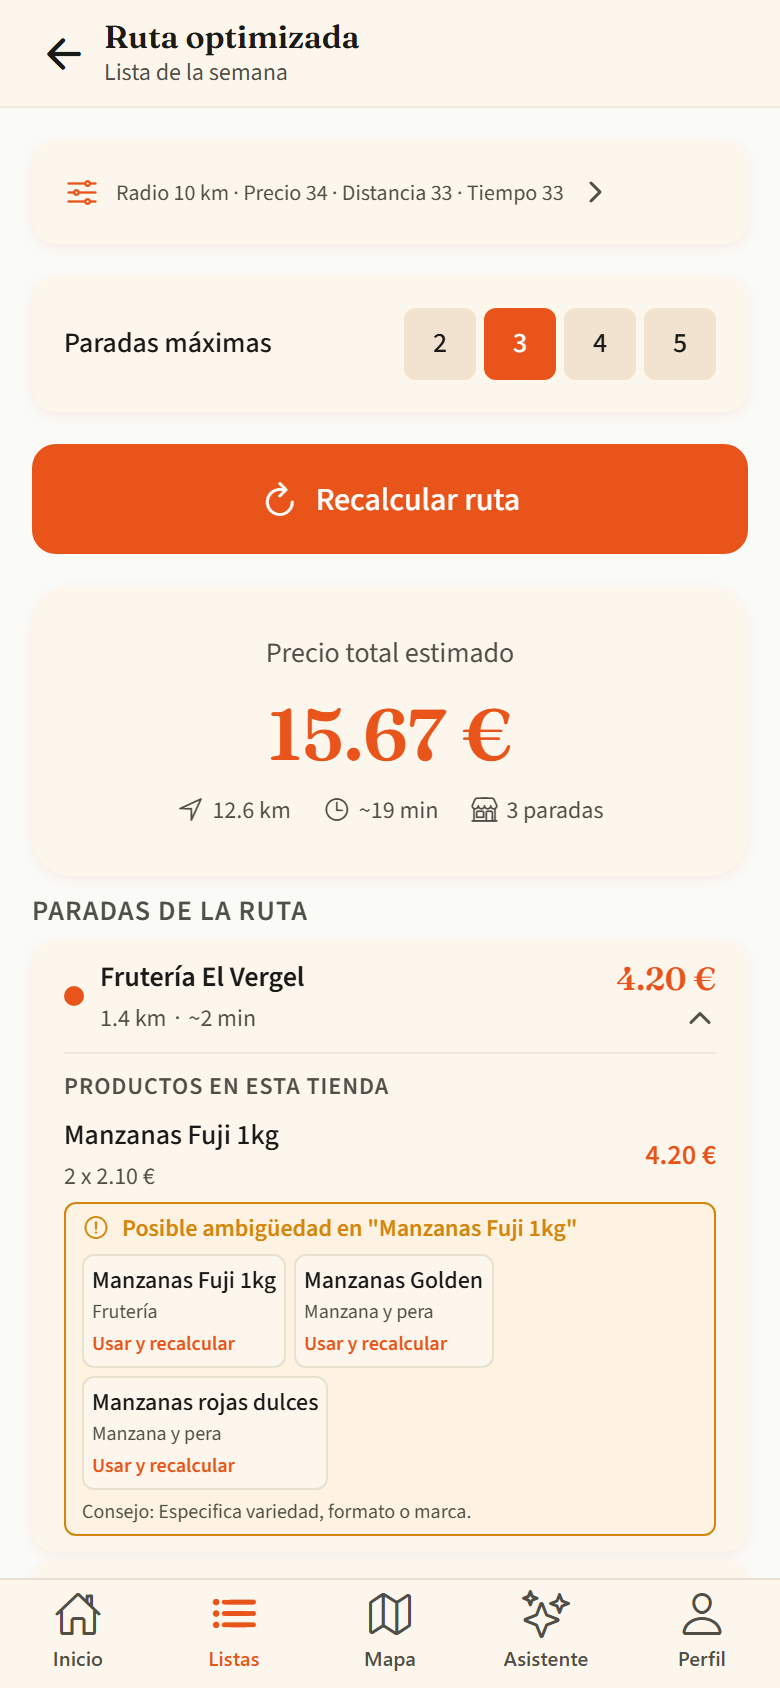
\includegraphics[width=0.30\textwidth]{diagramas/capturas/mobile-ruta.png}
\caption{M\'ovil --- Plantillas de lista (izquierda) y ruta optimizada (derecha)}
\label{fig:cap-mobile-plantillas-ruta}
\end{figure}

\begin{figure}[htbp]
\centering
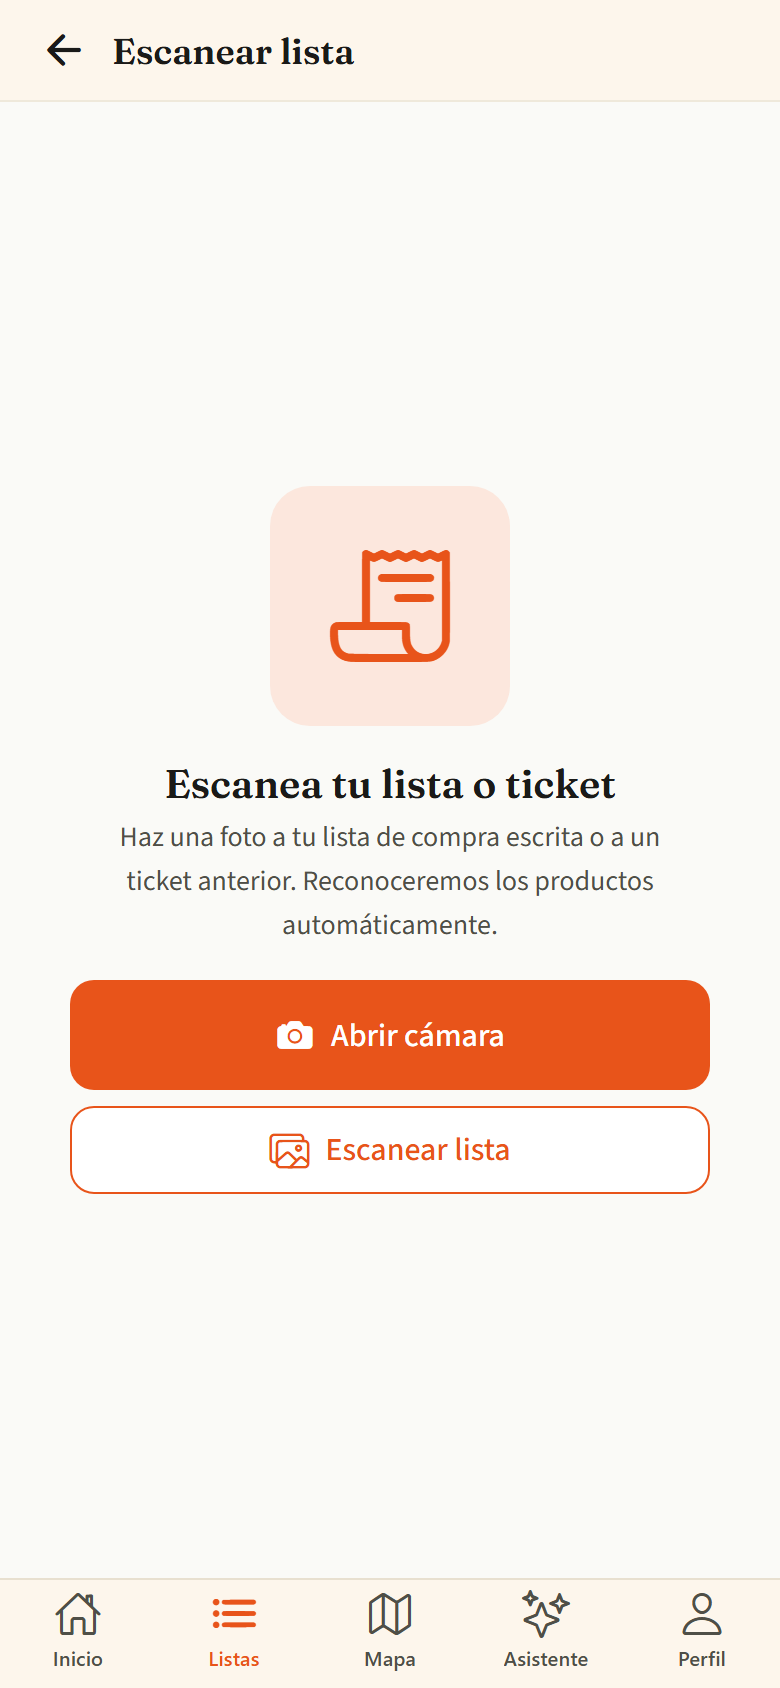
\includegraphics[width=0.30\textwidth]{diagramas/capturas/mobile-ocr-captura.png}
\hfill
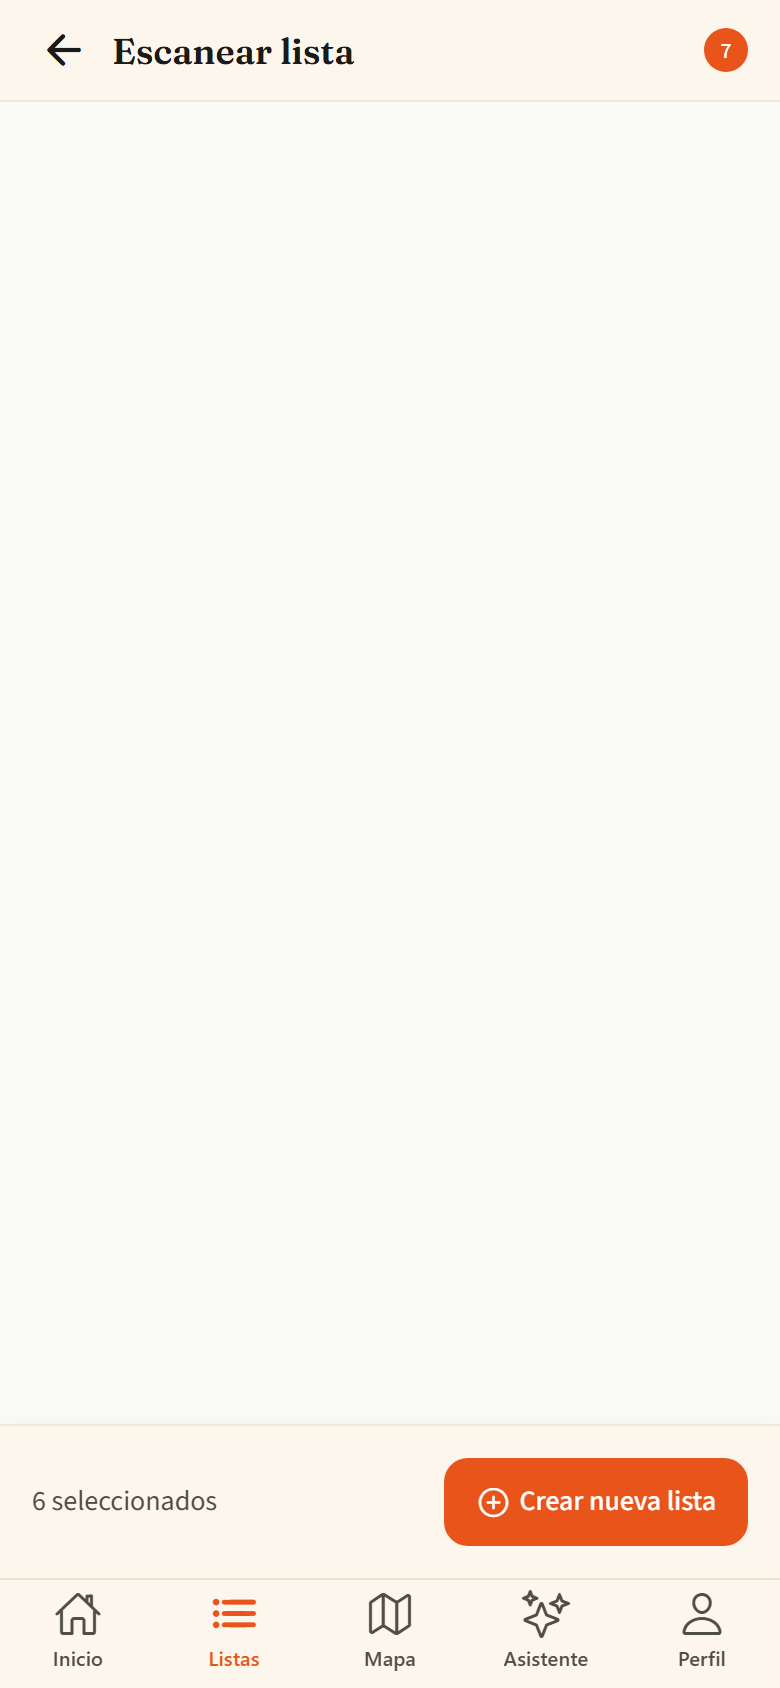
\includegraphics[width=0.30\textwidth]{diagramas/capturas/mobile-ocr-revision.png}
\caption{M\'ovil --- M\'odulo OCR: captura de ticket (izquierda) y revisi\'on de \'items (derecha)}
\label{fig:cap-mobile-ocr}
\end{figure}

\begin{figure}[htbp]
\centering
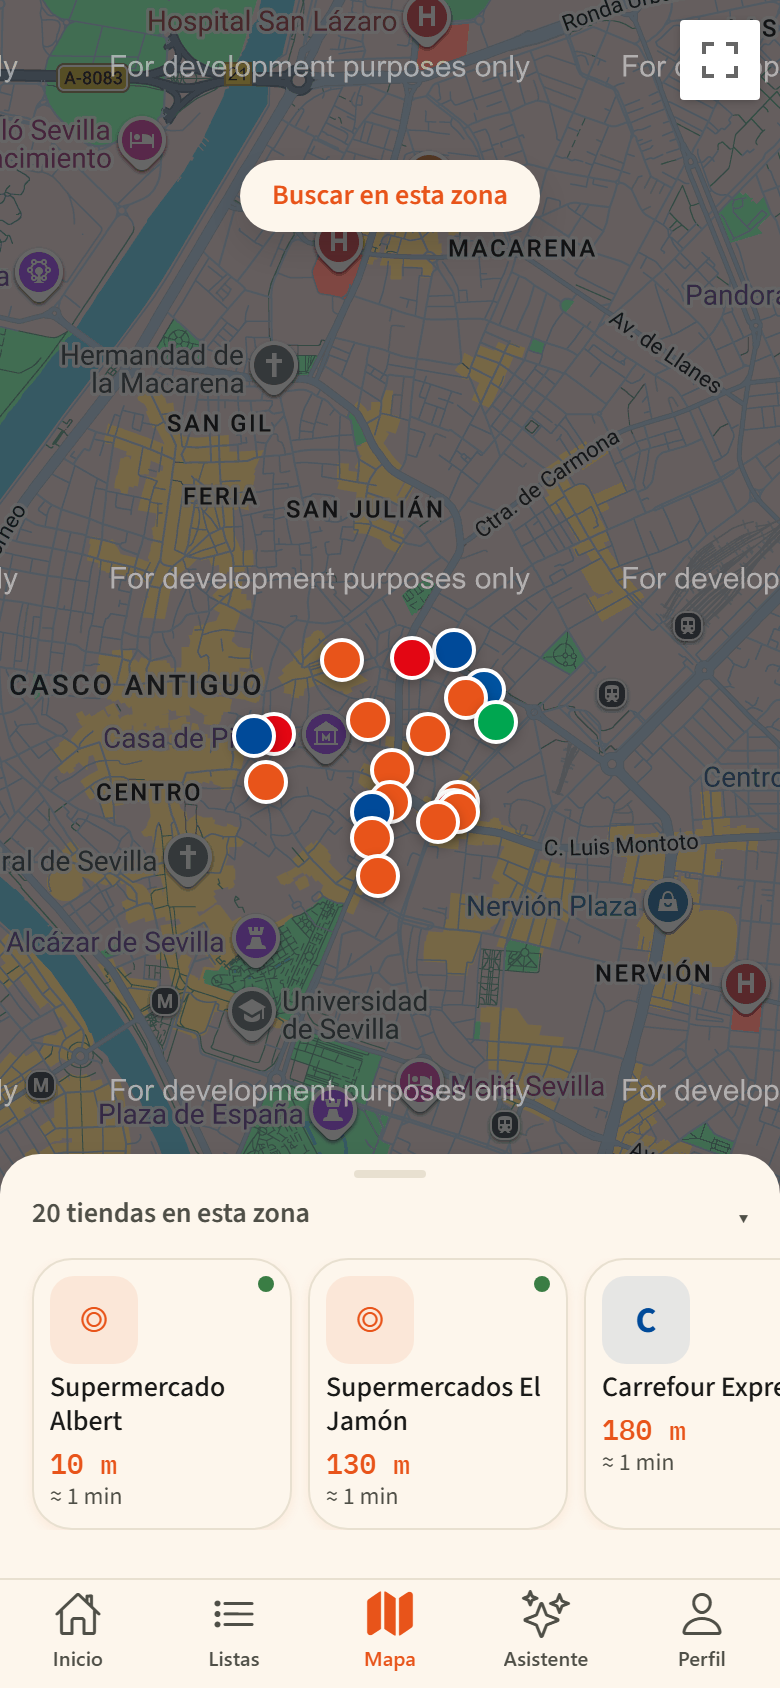
\includegraphics[width=0.30\textwidth]{diagramas/capturas/mobile-mapa.png}
\hfill
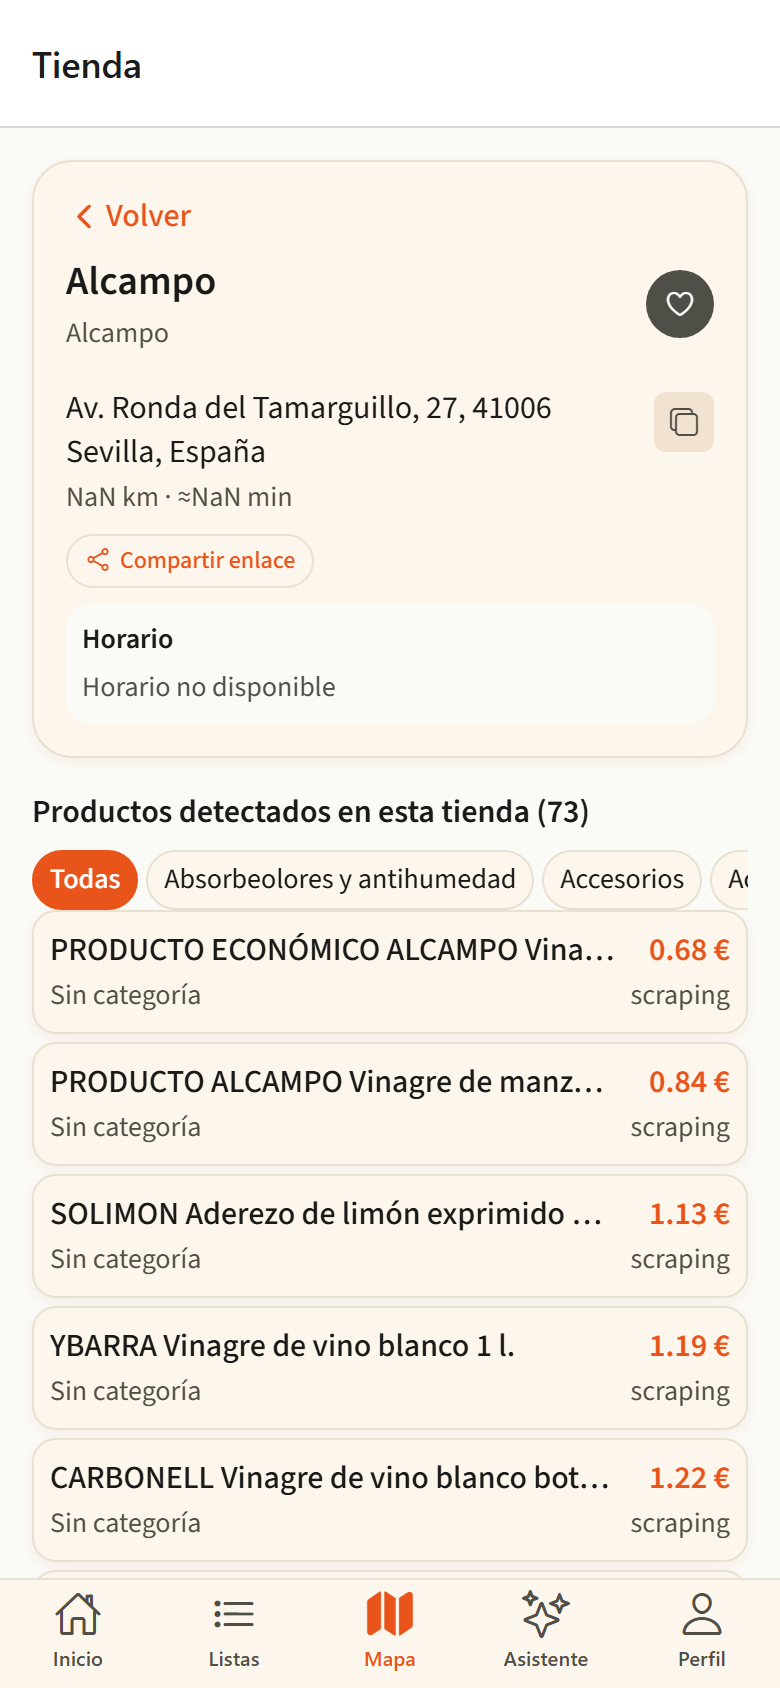
\includegraphics[width=0.30\textwidth]{diagramas/capturas/mobile-tienda-perfil.png}
\caption{M\'ovil --- Mapa de tiendas (izquierda) y perfil de tienda (derecha)}
\label{fig:cap-mobile-mapa}
\end{figure}

\begin{figure}[htbp]
\centering
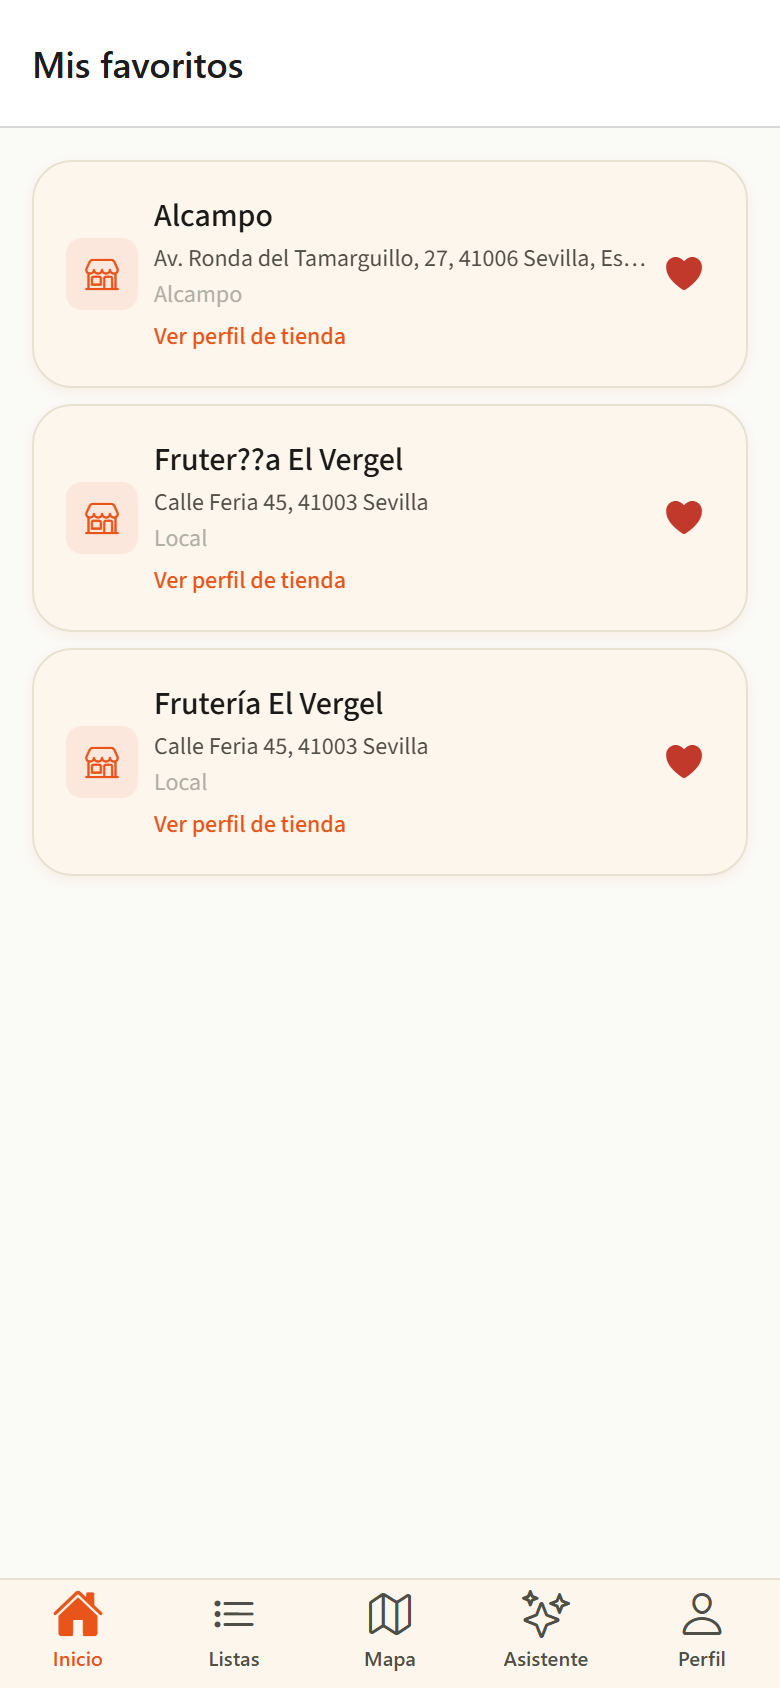
\includegraphics[width=0.30\textwidth]{diagramas/capturas/mobile-favoritas.png}
\hfill
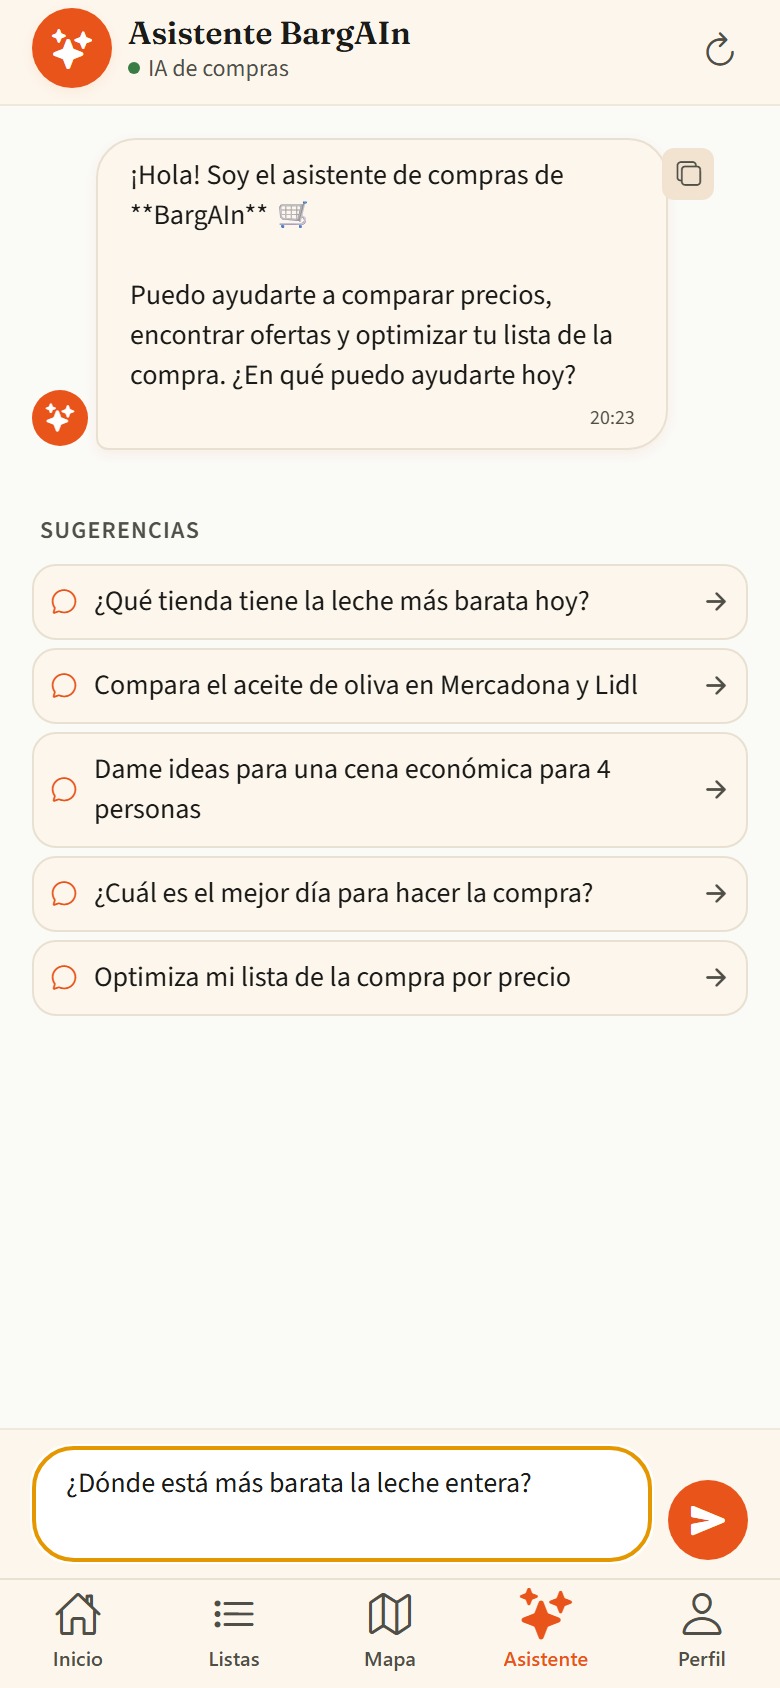
\includegraphics[width=0.30\textwidth]{diagramas/capturas/mobile-asistente.png}
\caption{M\'ovil --- Tiendas favoritas (izquierda) y asistente conversacional (derecha)}
\label{fig:cap-mobile-favoritas-asistente}
\end{figure}

\clearpage

\begin{figure}[htbp]
\centering
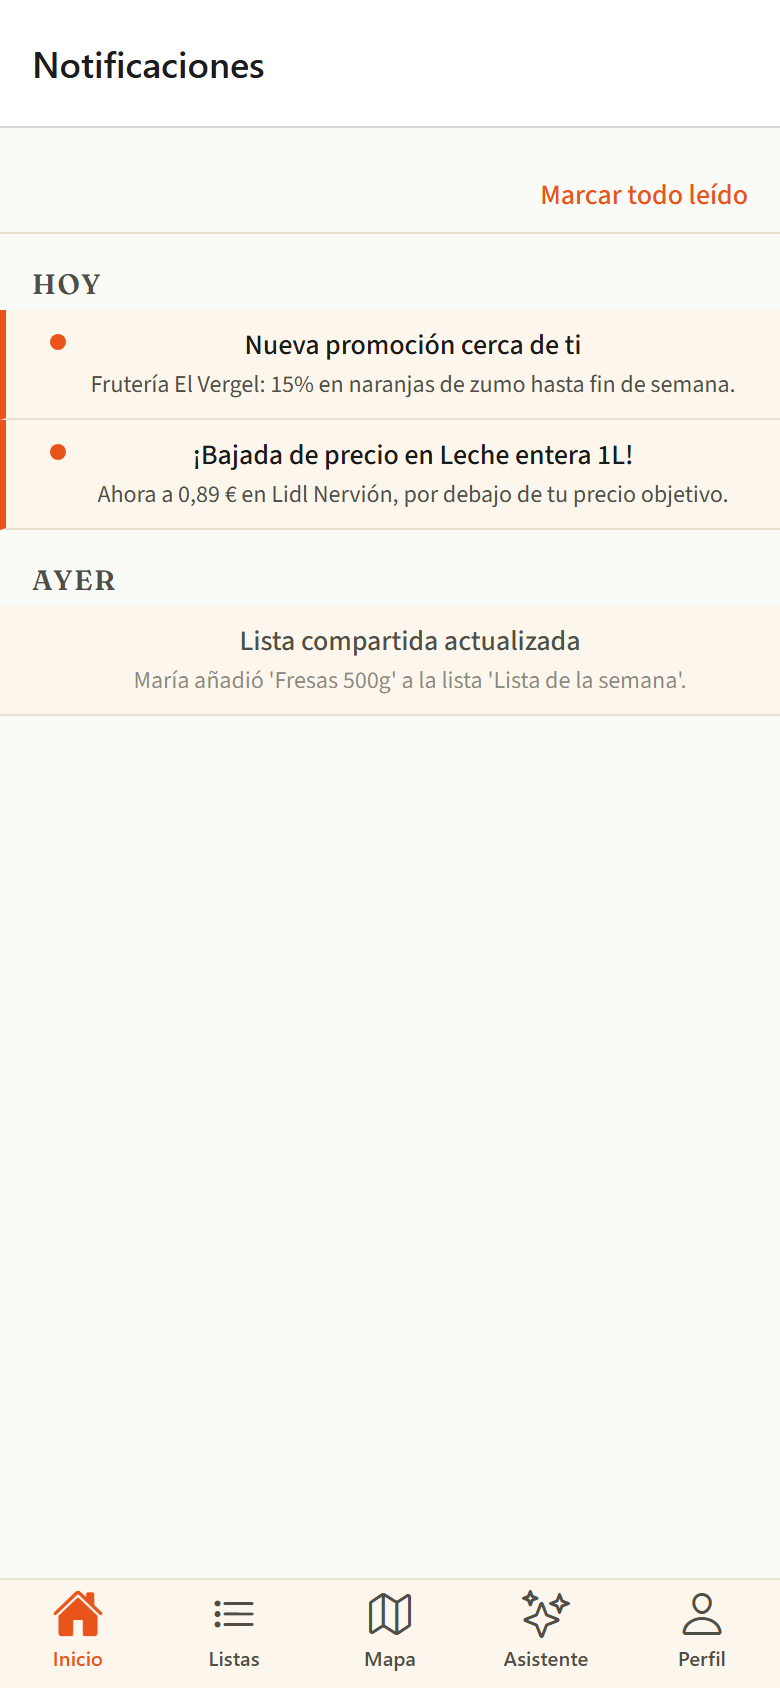
\includegraphics[width=0.30\textwidth]{diagramas/capturas/mobile-notificaciones.png}
\hfill
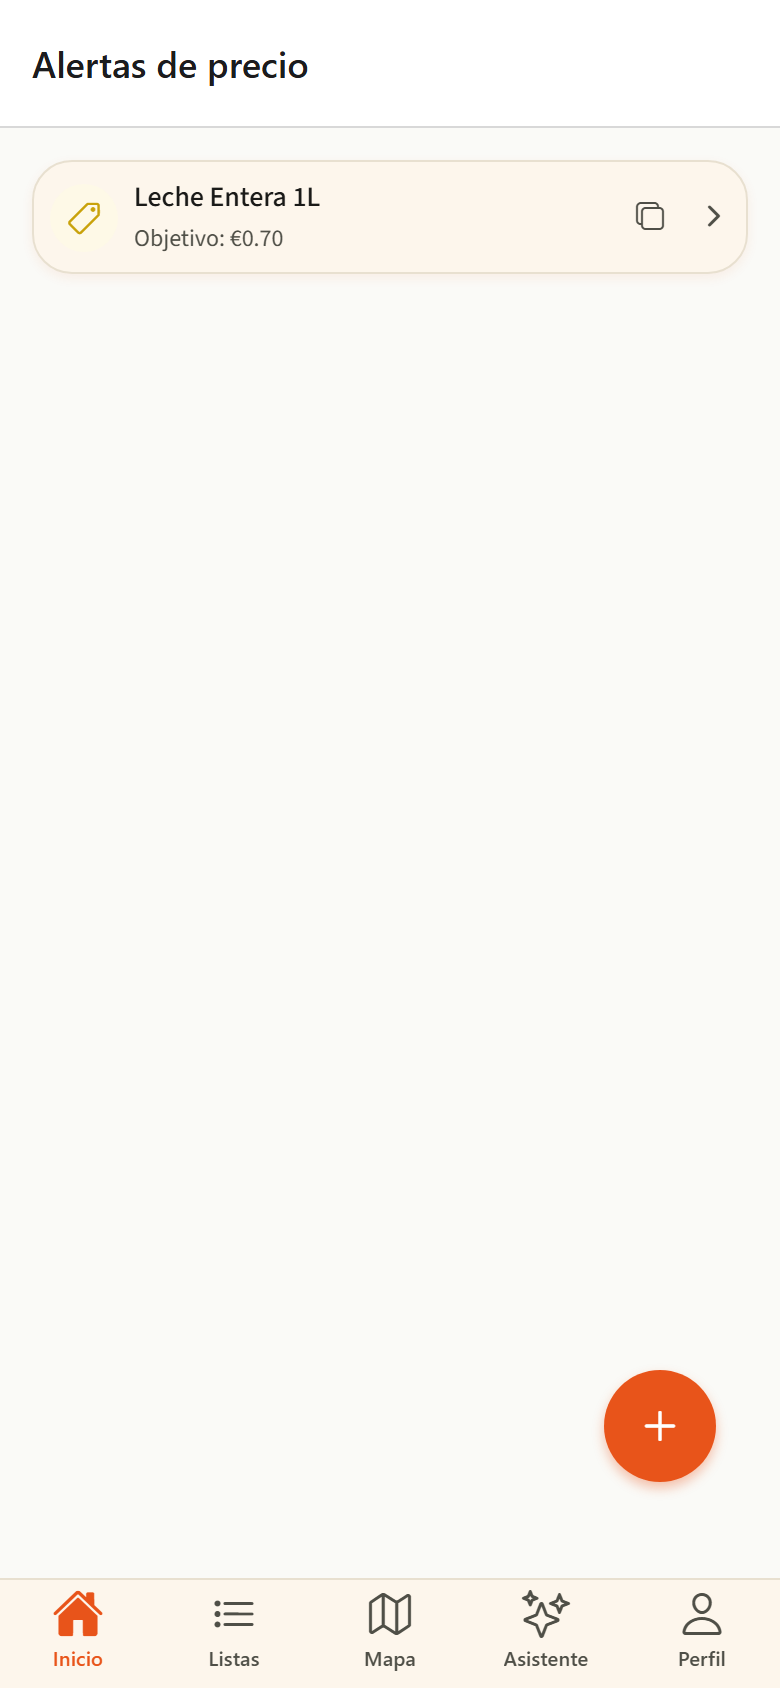
\includegraphics[width=0.30\textwidth]{diagramas/capturas/mobile-alertas.png}
\caption{M\'ovil --- Bandeja de notificaciones (izquierda) y alertas de precio (derecha)}
\label{fig:cap-mobile-notif-alertas}
\end{figure}

\begin{figure}[htbp]
\centering
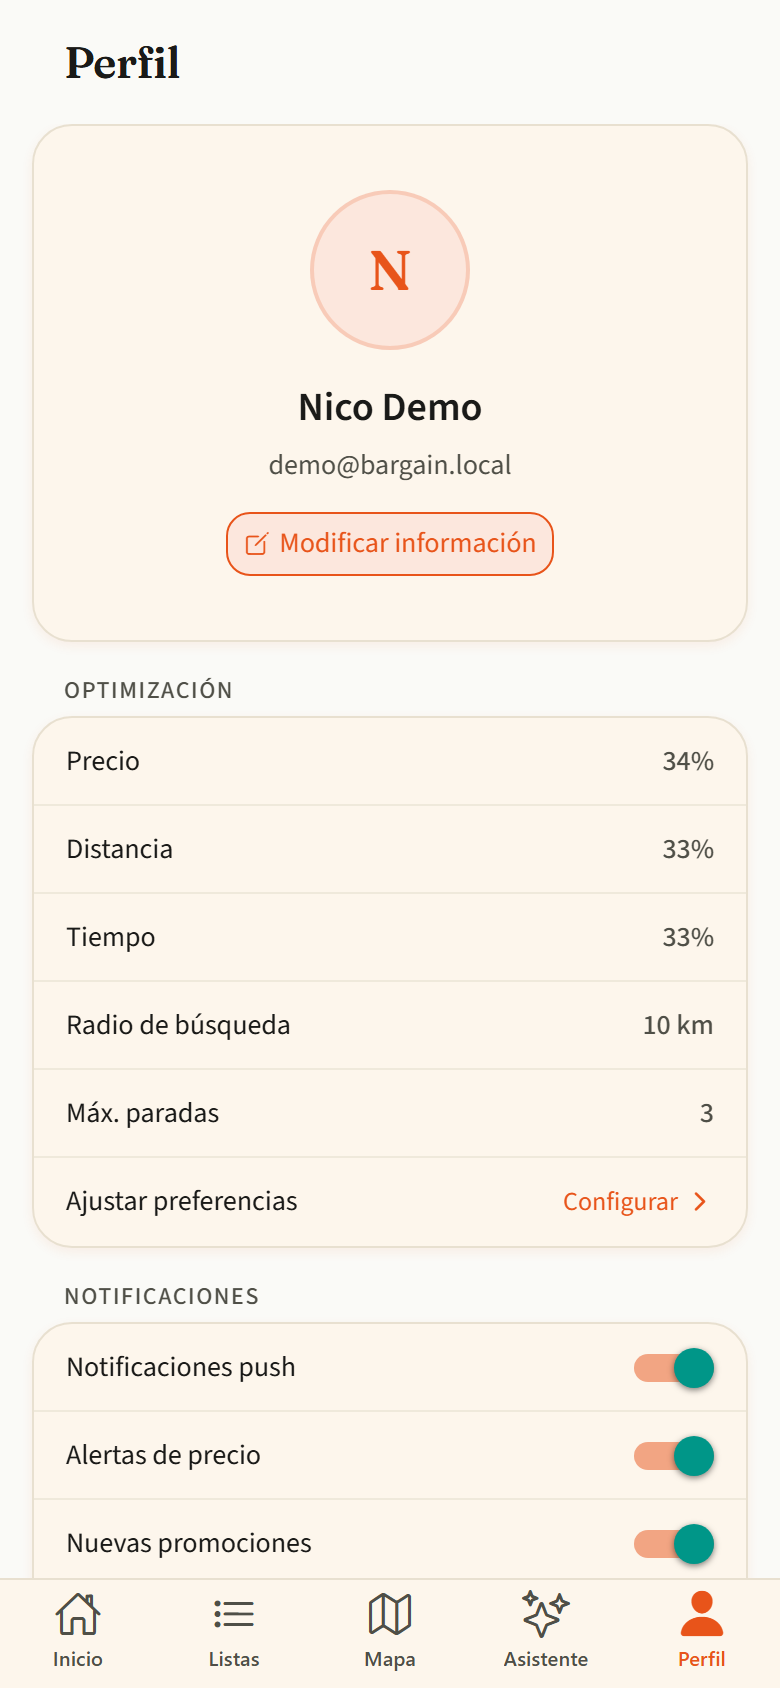
\includegraphics[width=0.30\textwidth]{diagramas/capturas/mobile-perfil.png}
\hfill
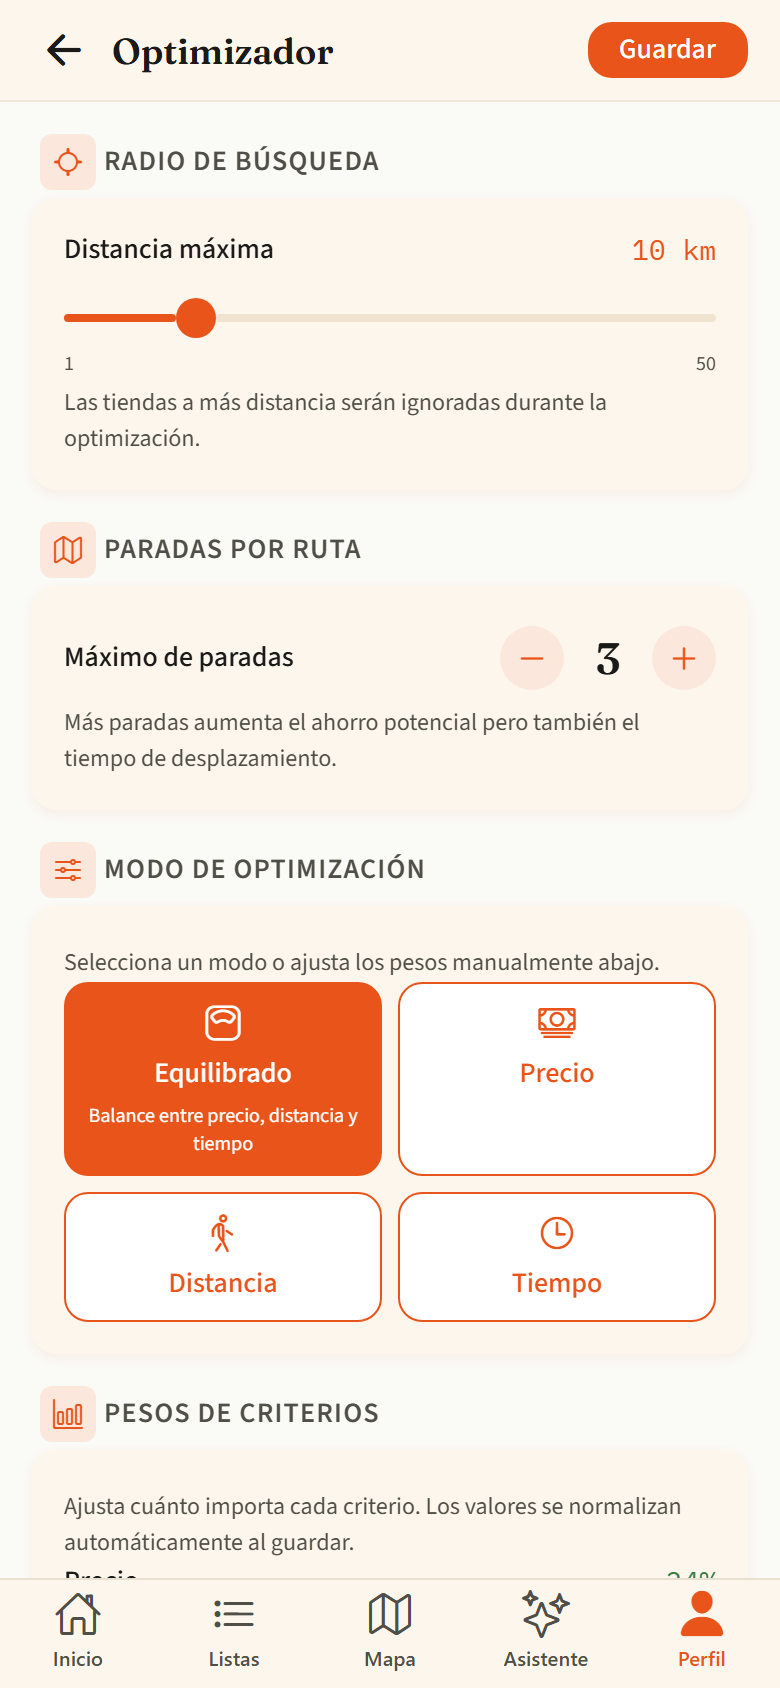
\includegraphics[width=0.30\textwidth]{diagramas/capturas/mobile-config-optimizador.png}
\caption{M\'ovil --- Perfil de usuario (izquierda) y configuraci\'on del optimizador (derecha)}
\label{fig:cap-mobile-perfil-config}
\end{figure}

\begin{figure}[htbp]
\centering
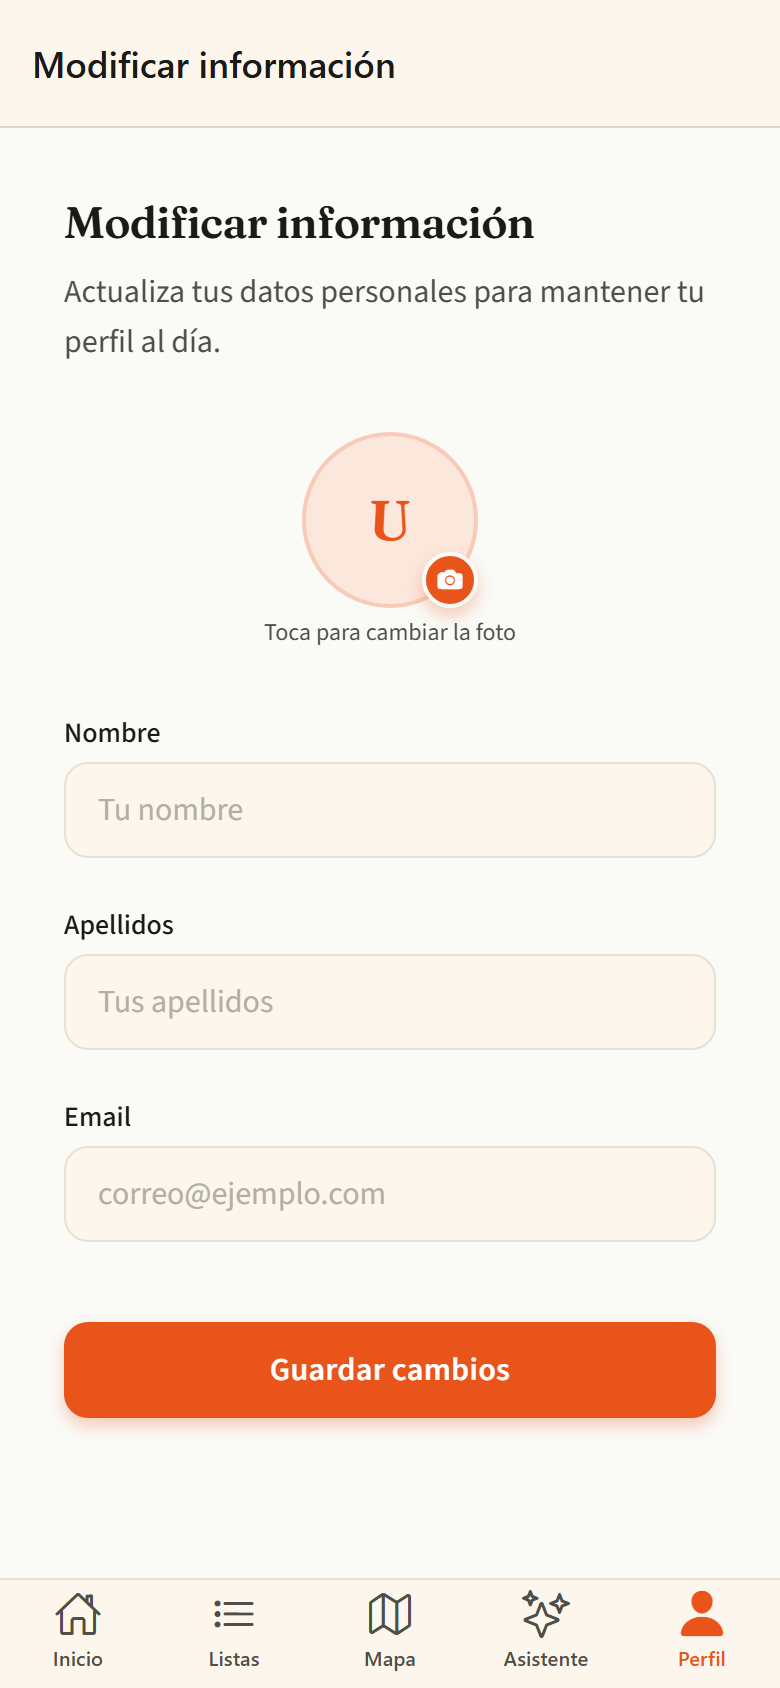
\includegraphics[width=0.30\textwidth]{diagramas/capturas/mobile-editar-perfil.png}
\hfill
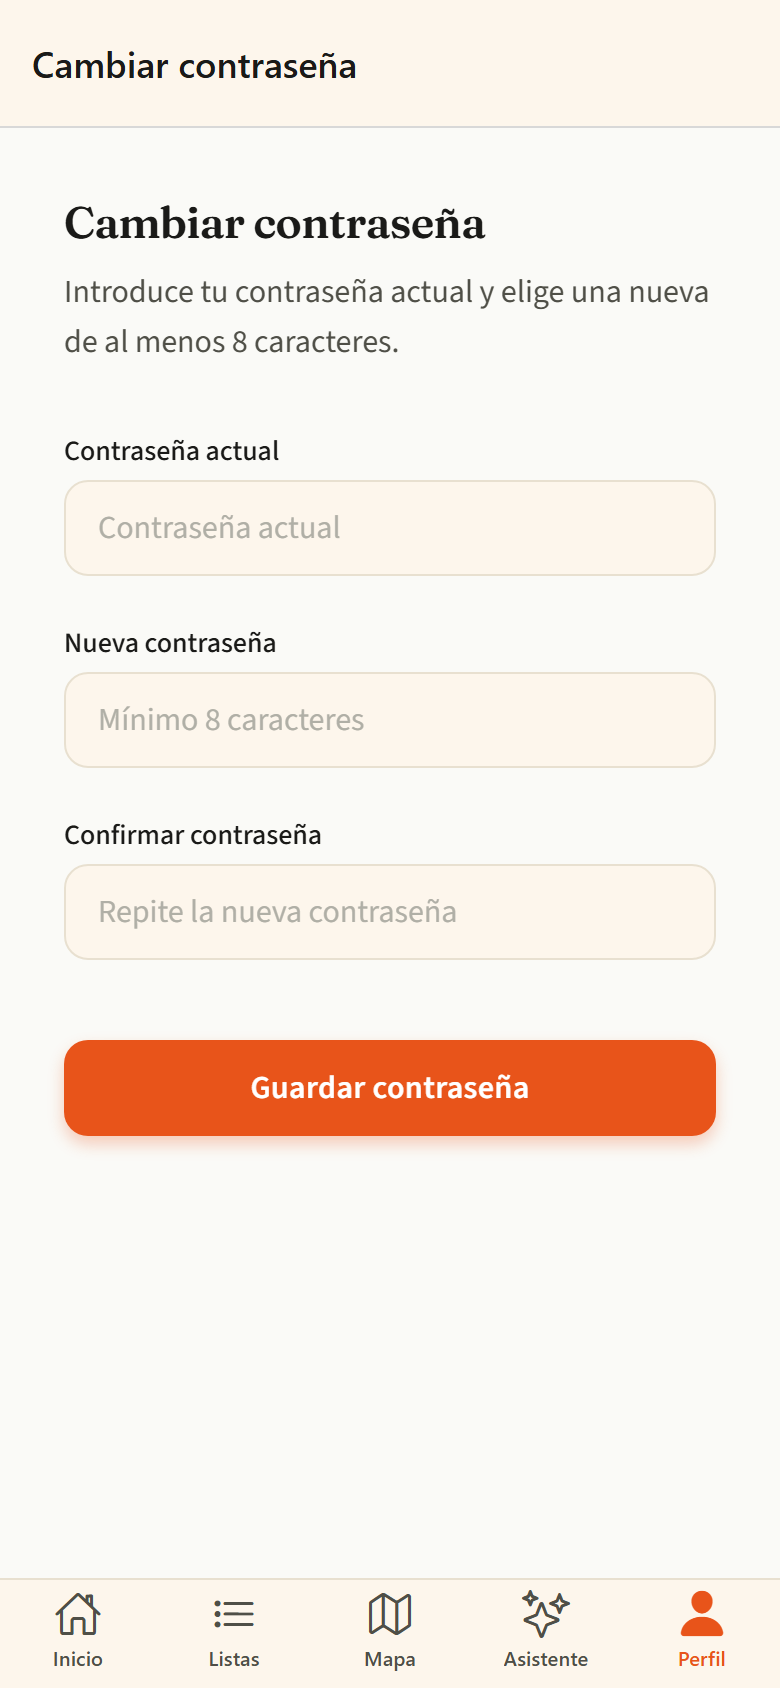
\includegraphics[width=0.30\textwidth]{diagramas/capturas/mobile-cambiar-password.png}
\caption{M\'ovil --- Edici\'on de perfil (izquierda) y cambio de contrase\~na (derecha)}
\label{fig:cap-mobile-editar-password}
\end{figure}

\clearpage

\subsection{Aplicaci\'on web (usuario)}\label{subsec:galeria-web}

\begin{figure}[htbp]
\centering
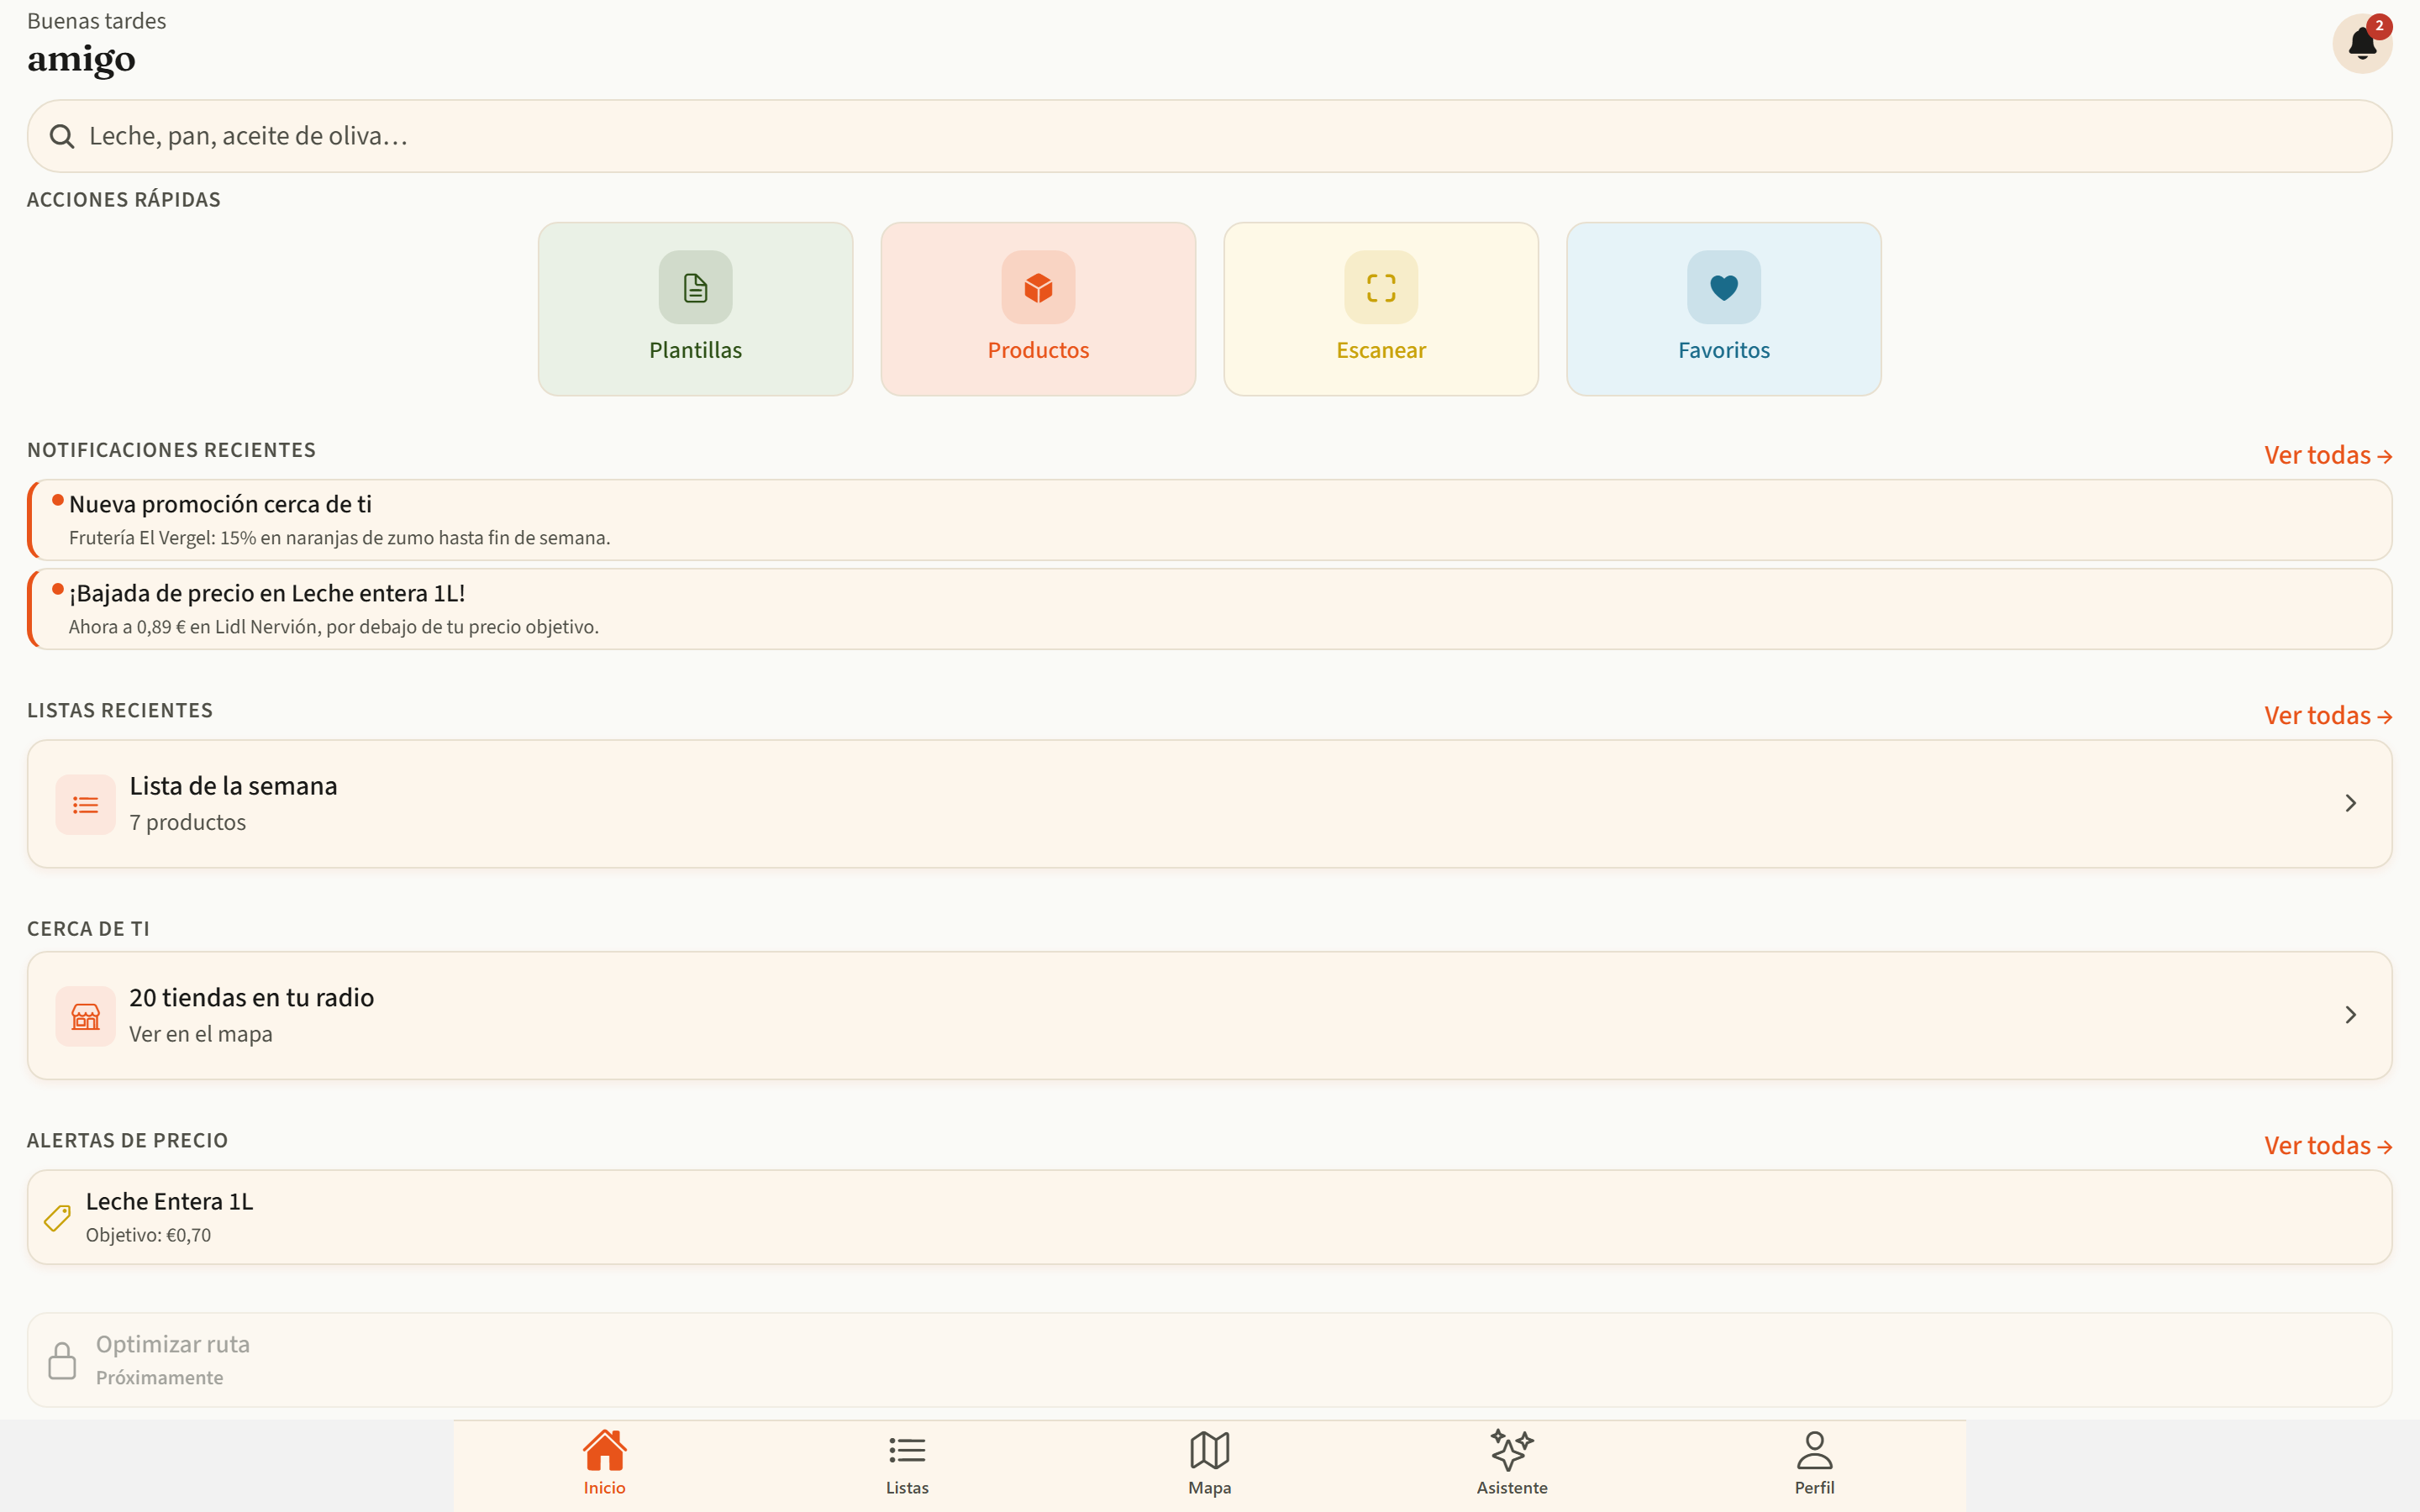
\includegraphics[width=0.46\textwidth]{diagramas/capturas/web-home.png}
\hfill
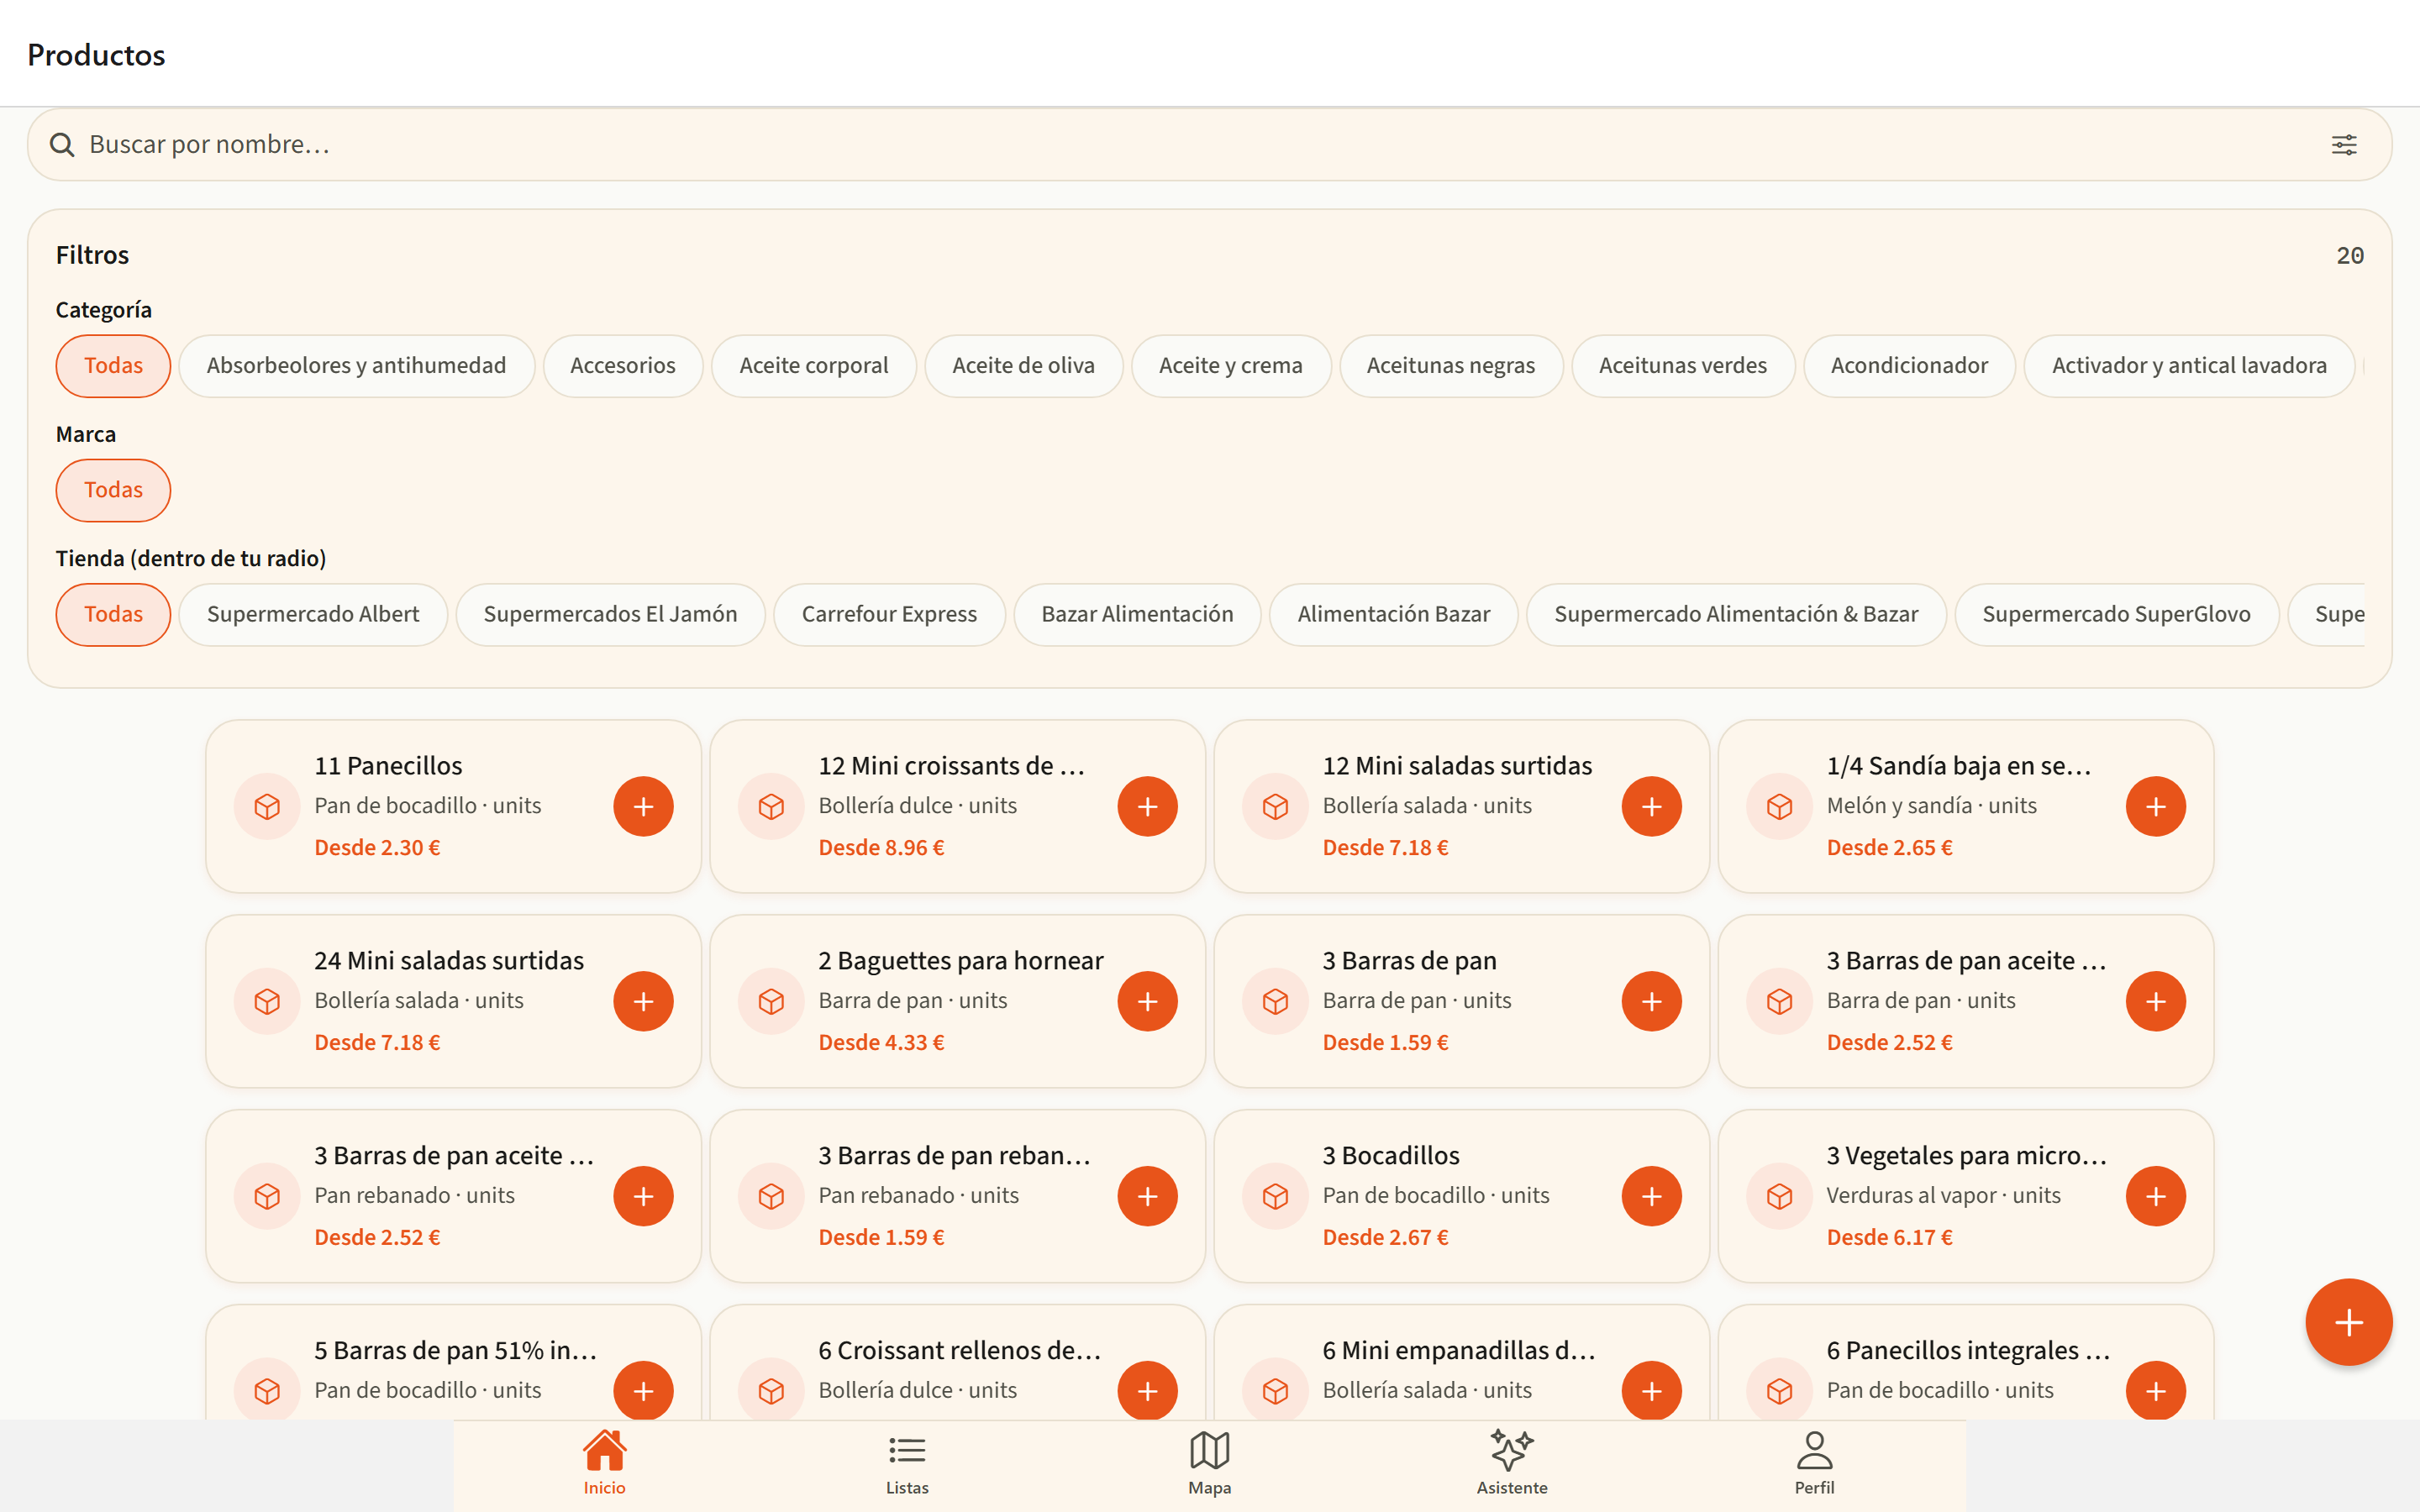
\includegraphics[width=0.46\textwidth]{diagramas/capturas/web-catalogo.png}
\caption{Web --- Pantalla principal con accesos horizontales (izquierda) y cat\'alogo en rejilla
multicolumna con \texttt{Cmd/Ctrl+K} (derecha)}
\label{fig:cap-web-home-catalogo}
\end{figure}

\begin{figure}[htbp]
\centering
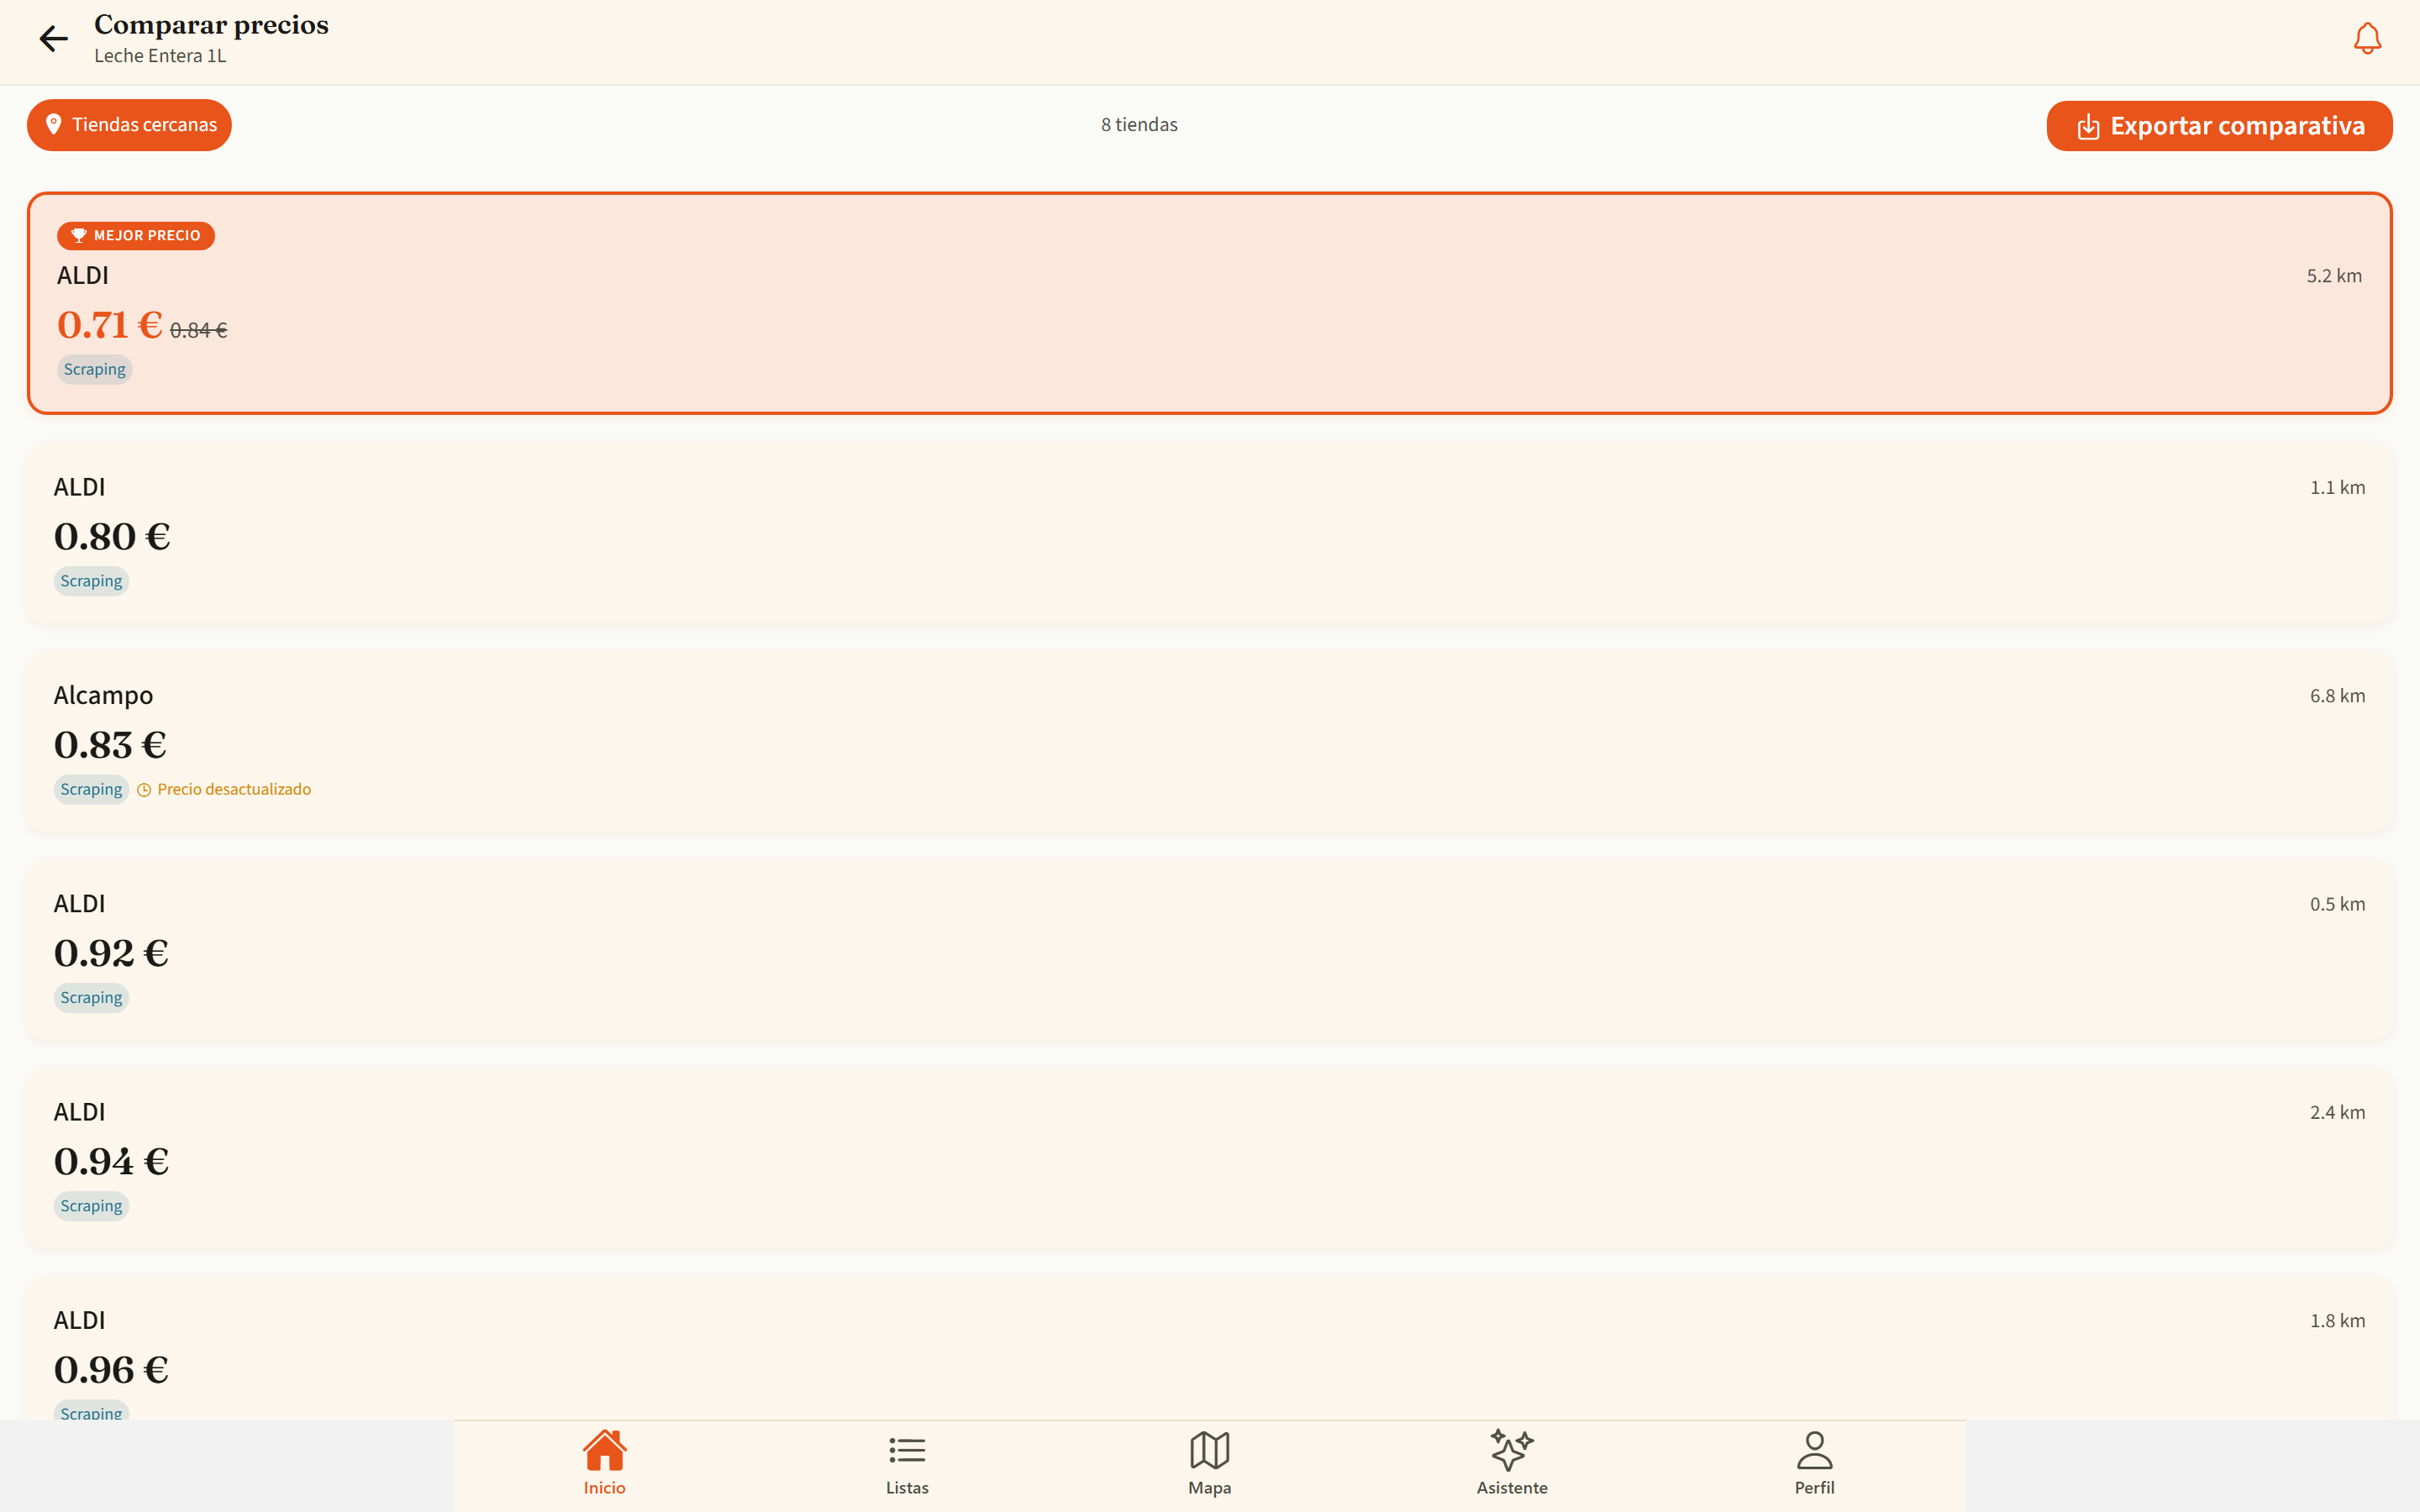
\includegraphics[width=0.46\textwidth]{diagramas/capturas/web-comparativa.png}
\hfill
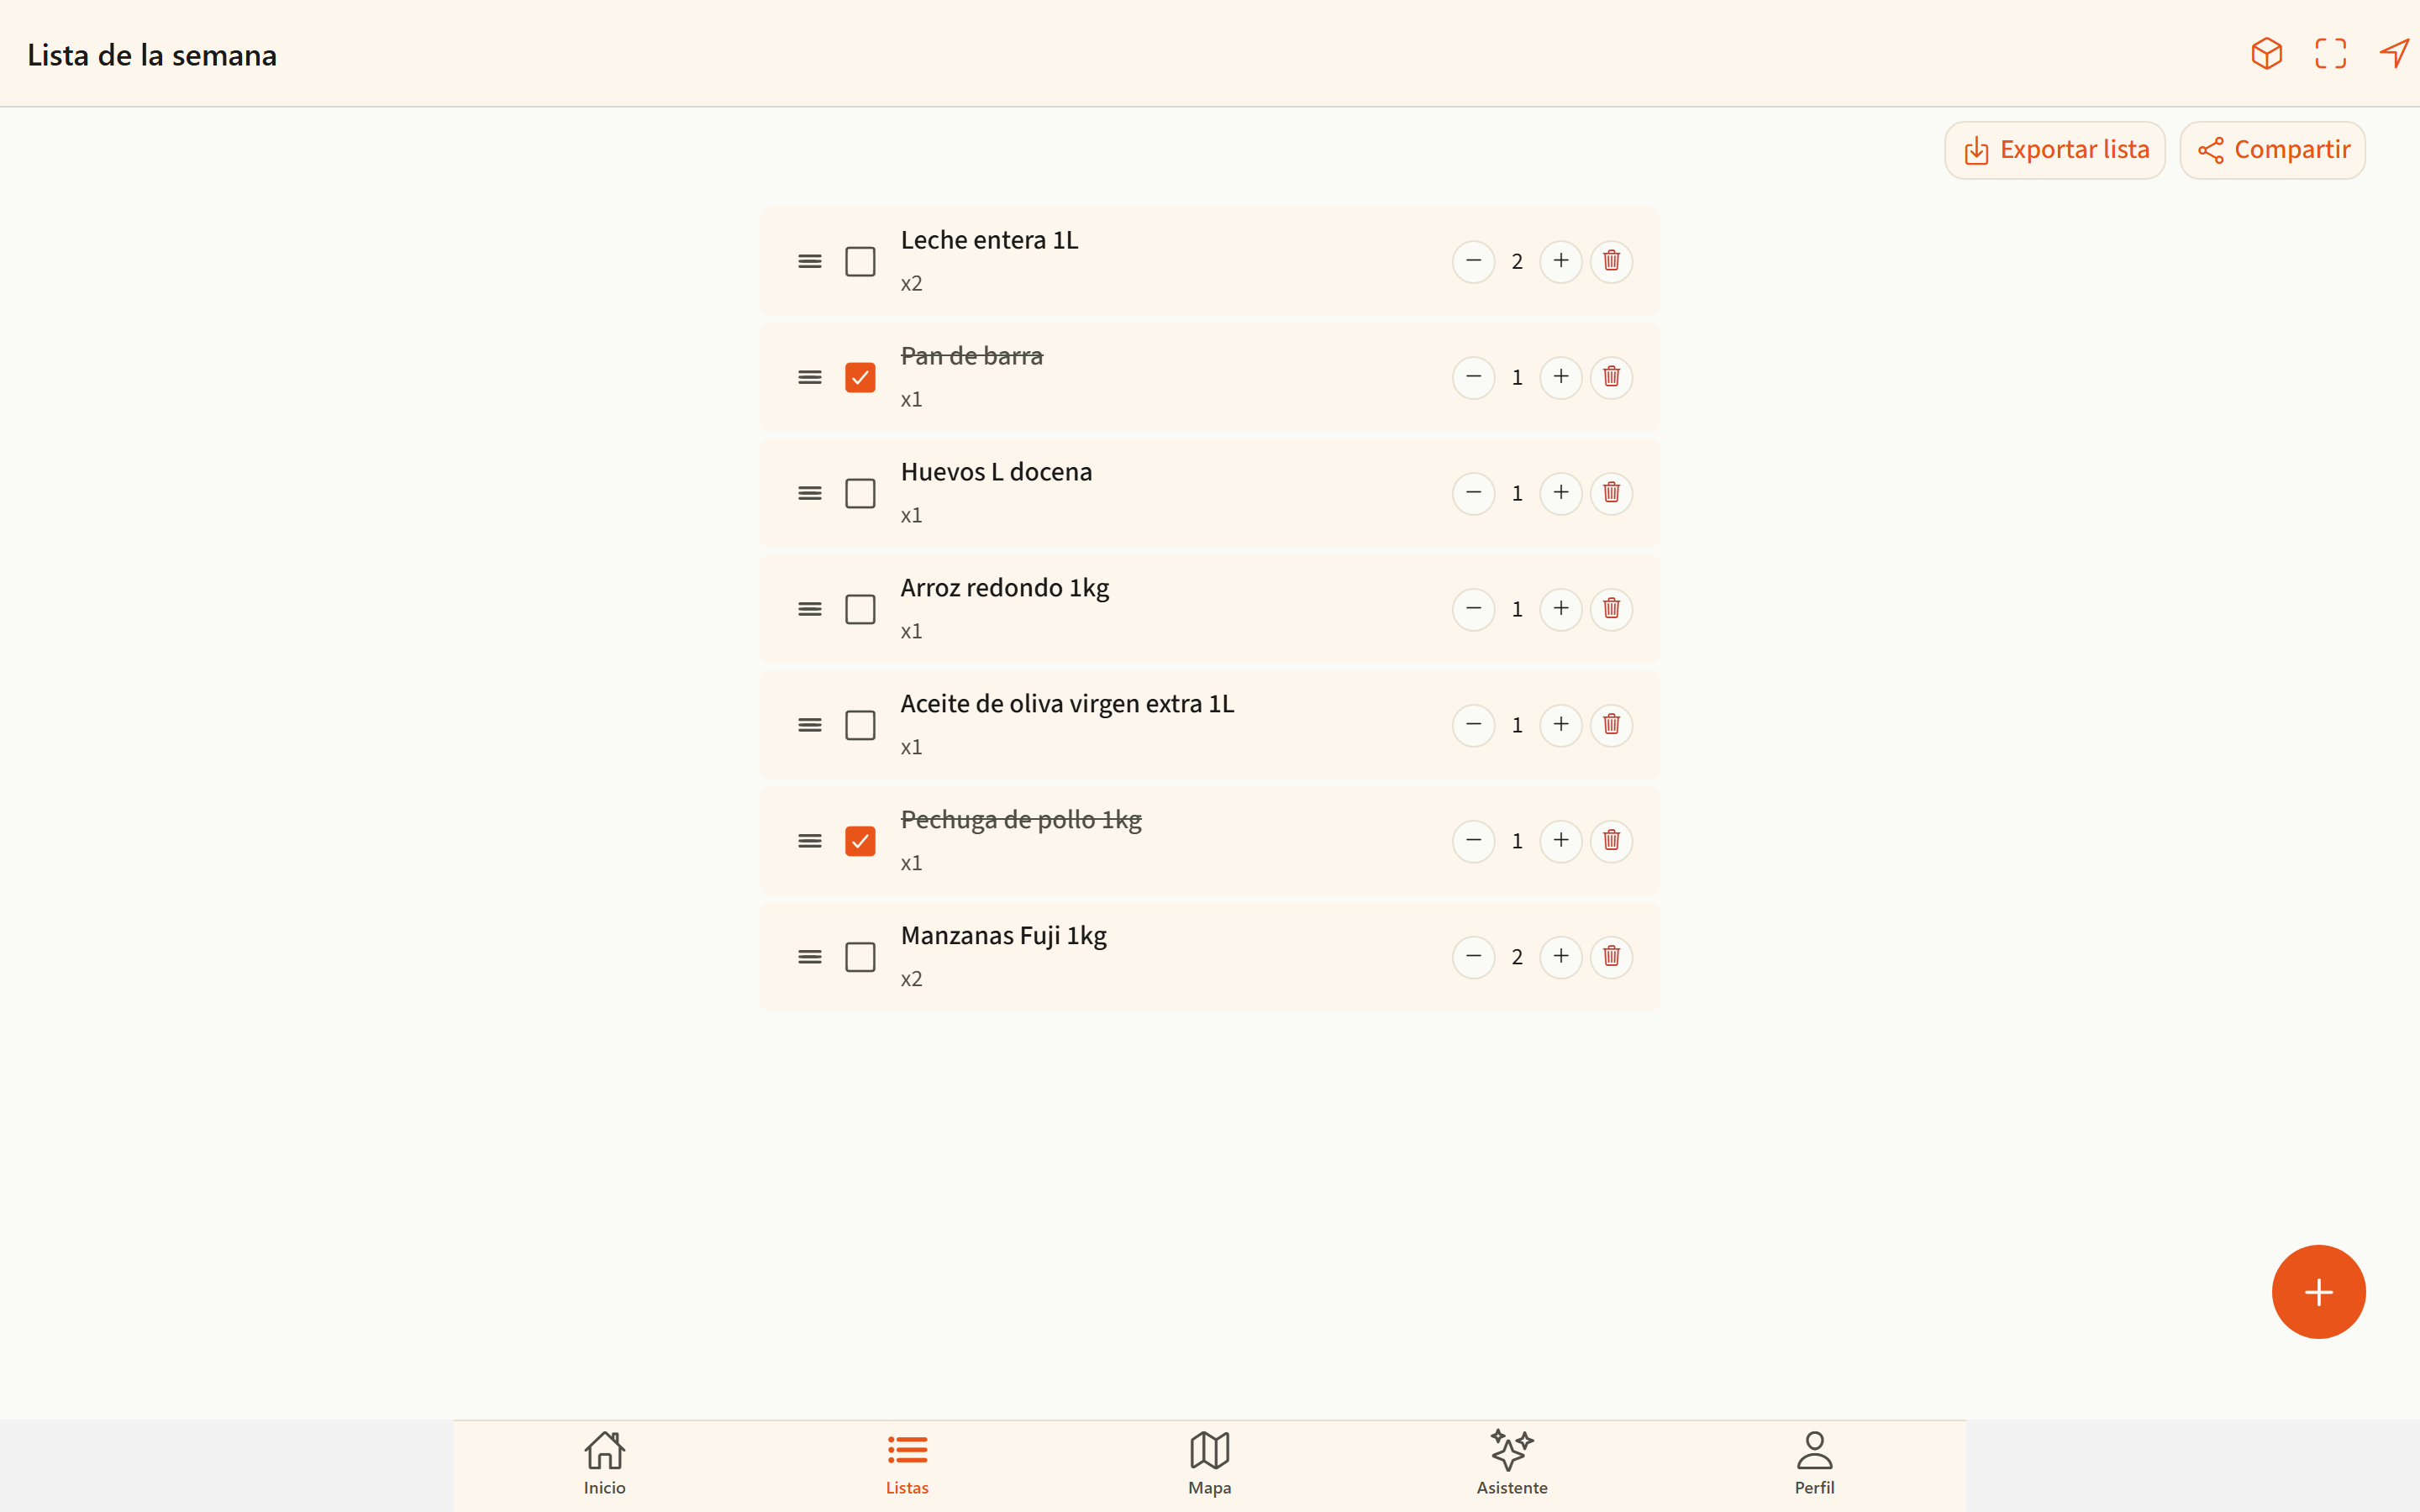
\includegraphics[width=0.46\textwidth]{diagramas/capturas/web-lista-detalle.png}
\caption{Web --- Comparativa de precios con cabecera fija y exportaci\'on CSV (izquierda) y detalle
de lista con reordenado \emph{drag-and-drop} y exportaci\'on (derecha)}
\label{fig:cap-web-comparativa-lista}
\end{figure}

\begin{figure}[htbp]
\centering
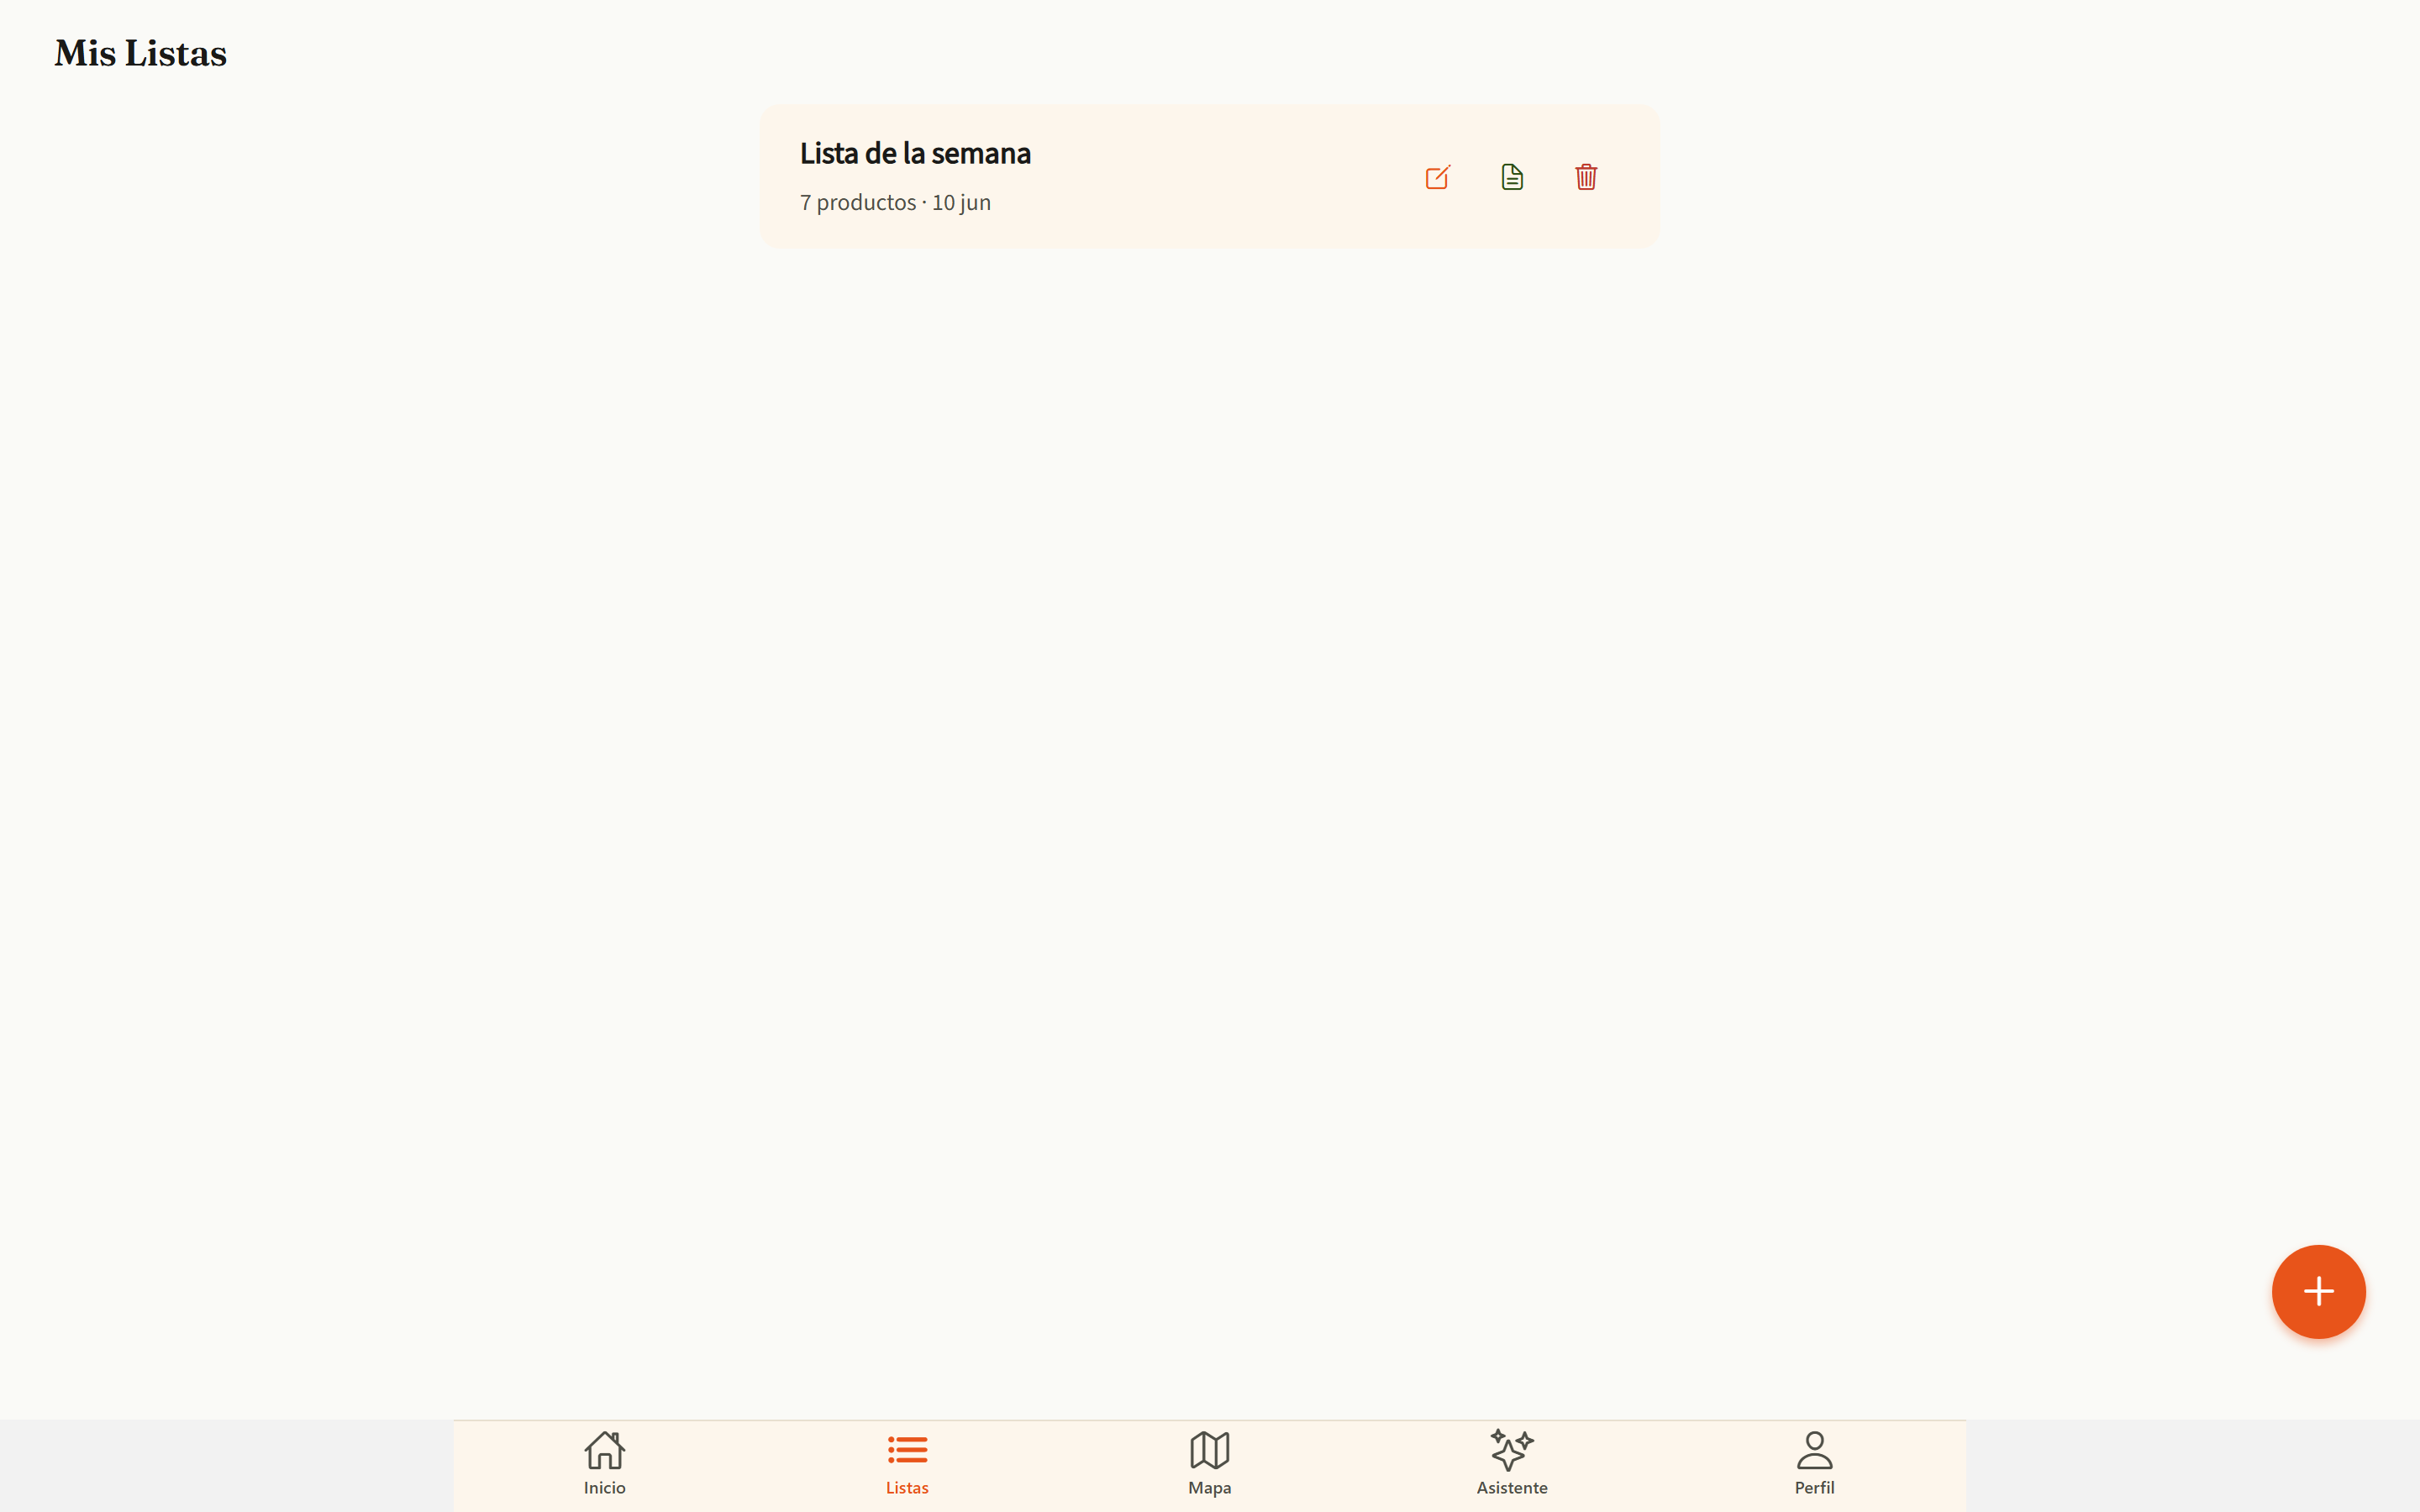
\includegraphics[width=0.46\textwidth]{diagramas/capturas/web-listas.png}
\hfill
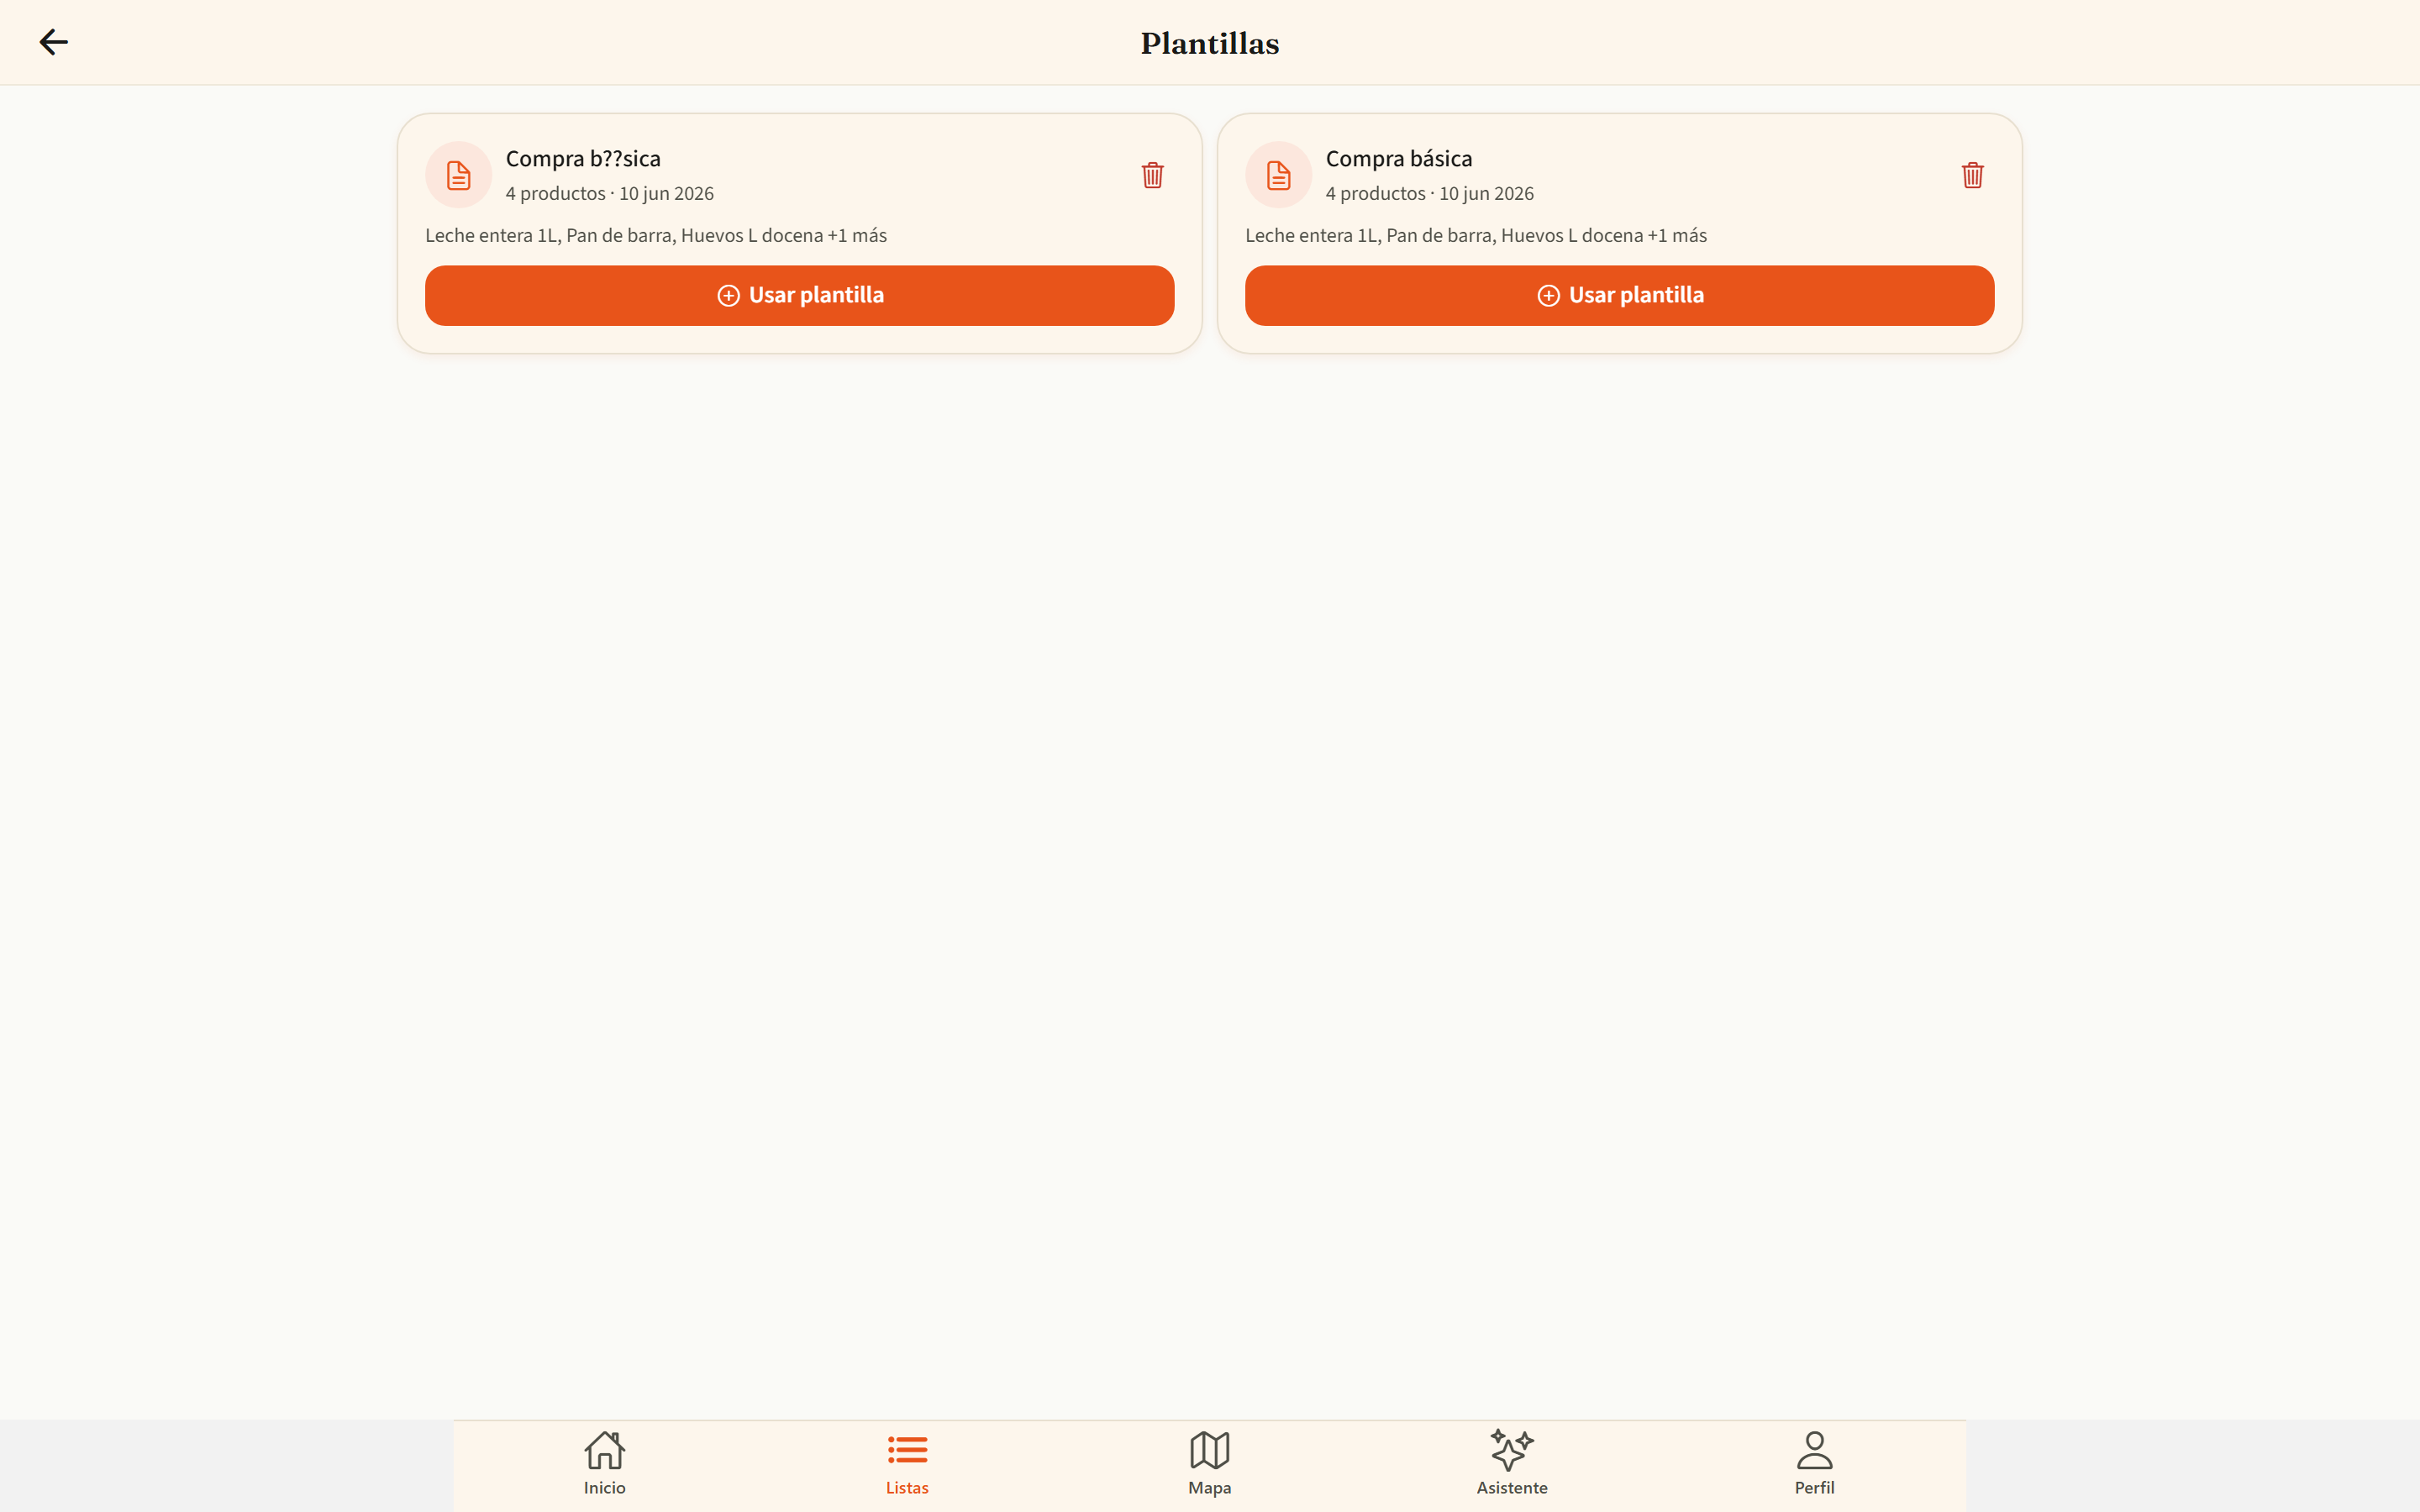
\includegraphics[width=0.46\textwidth]{diagramas/capturas/web-plantillas.png}
\caption{Web --- Listas (izquierda) y plantillas (derecha) con rejilla responsive}
\label{fig:cap-web-listas-plantillas}
\end{figure}

\begin{figure}[htbp]
\centering
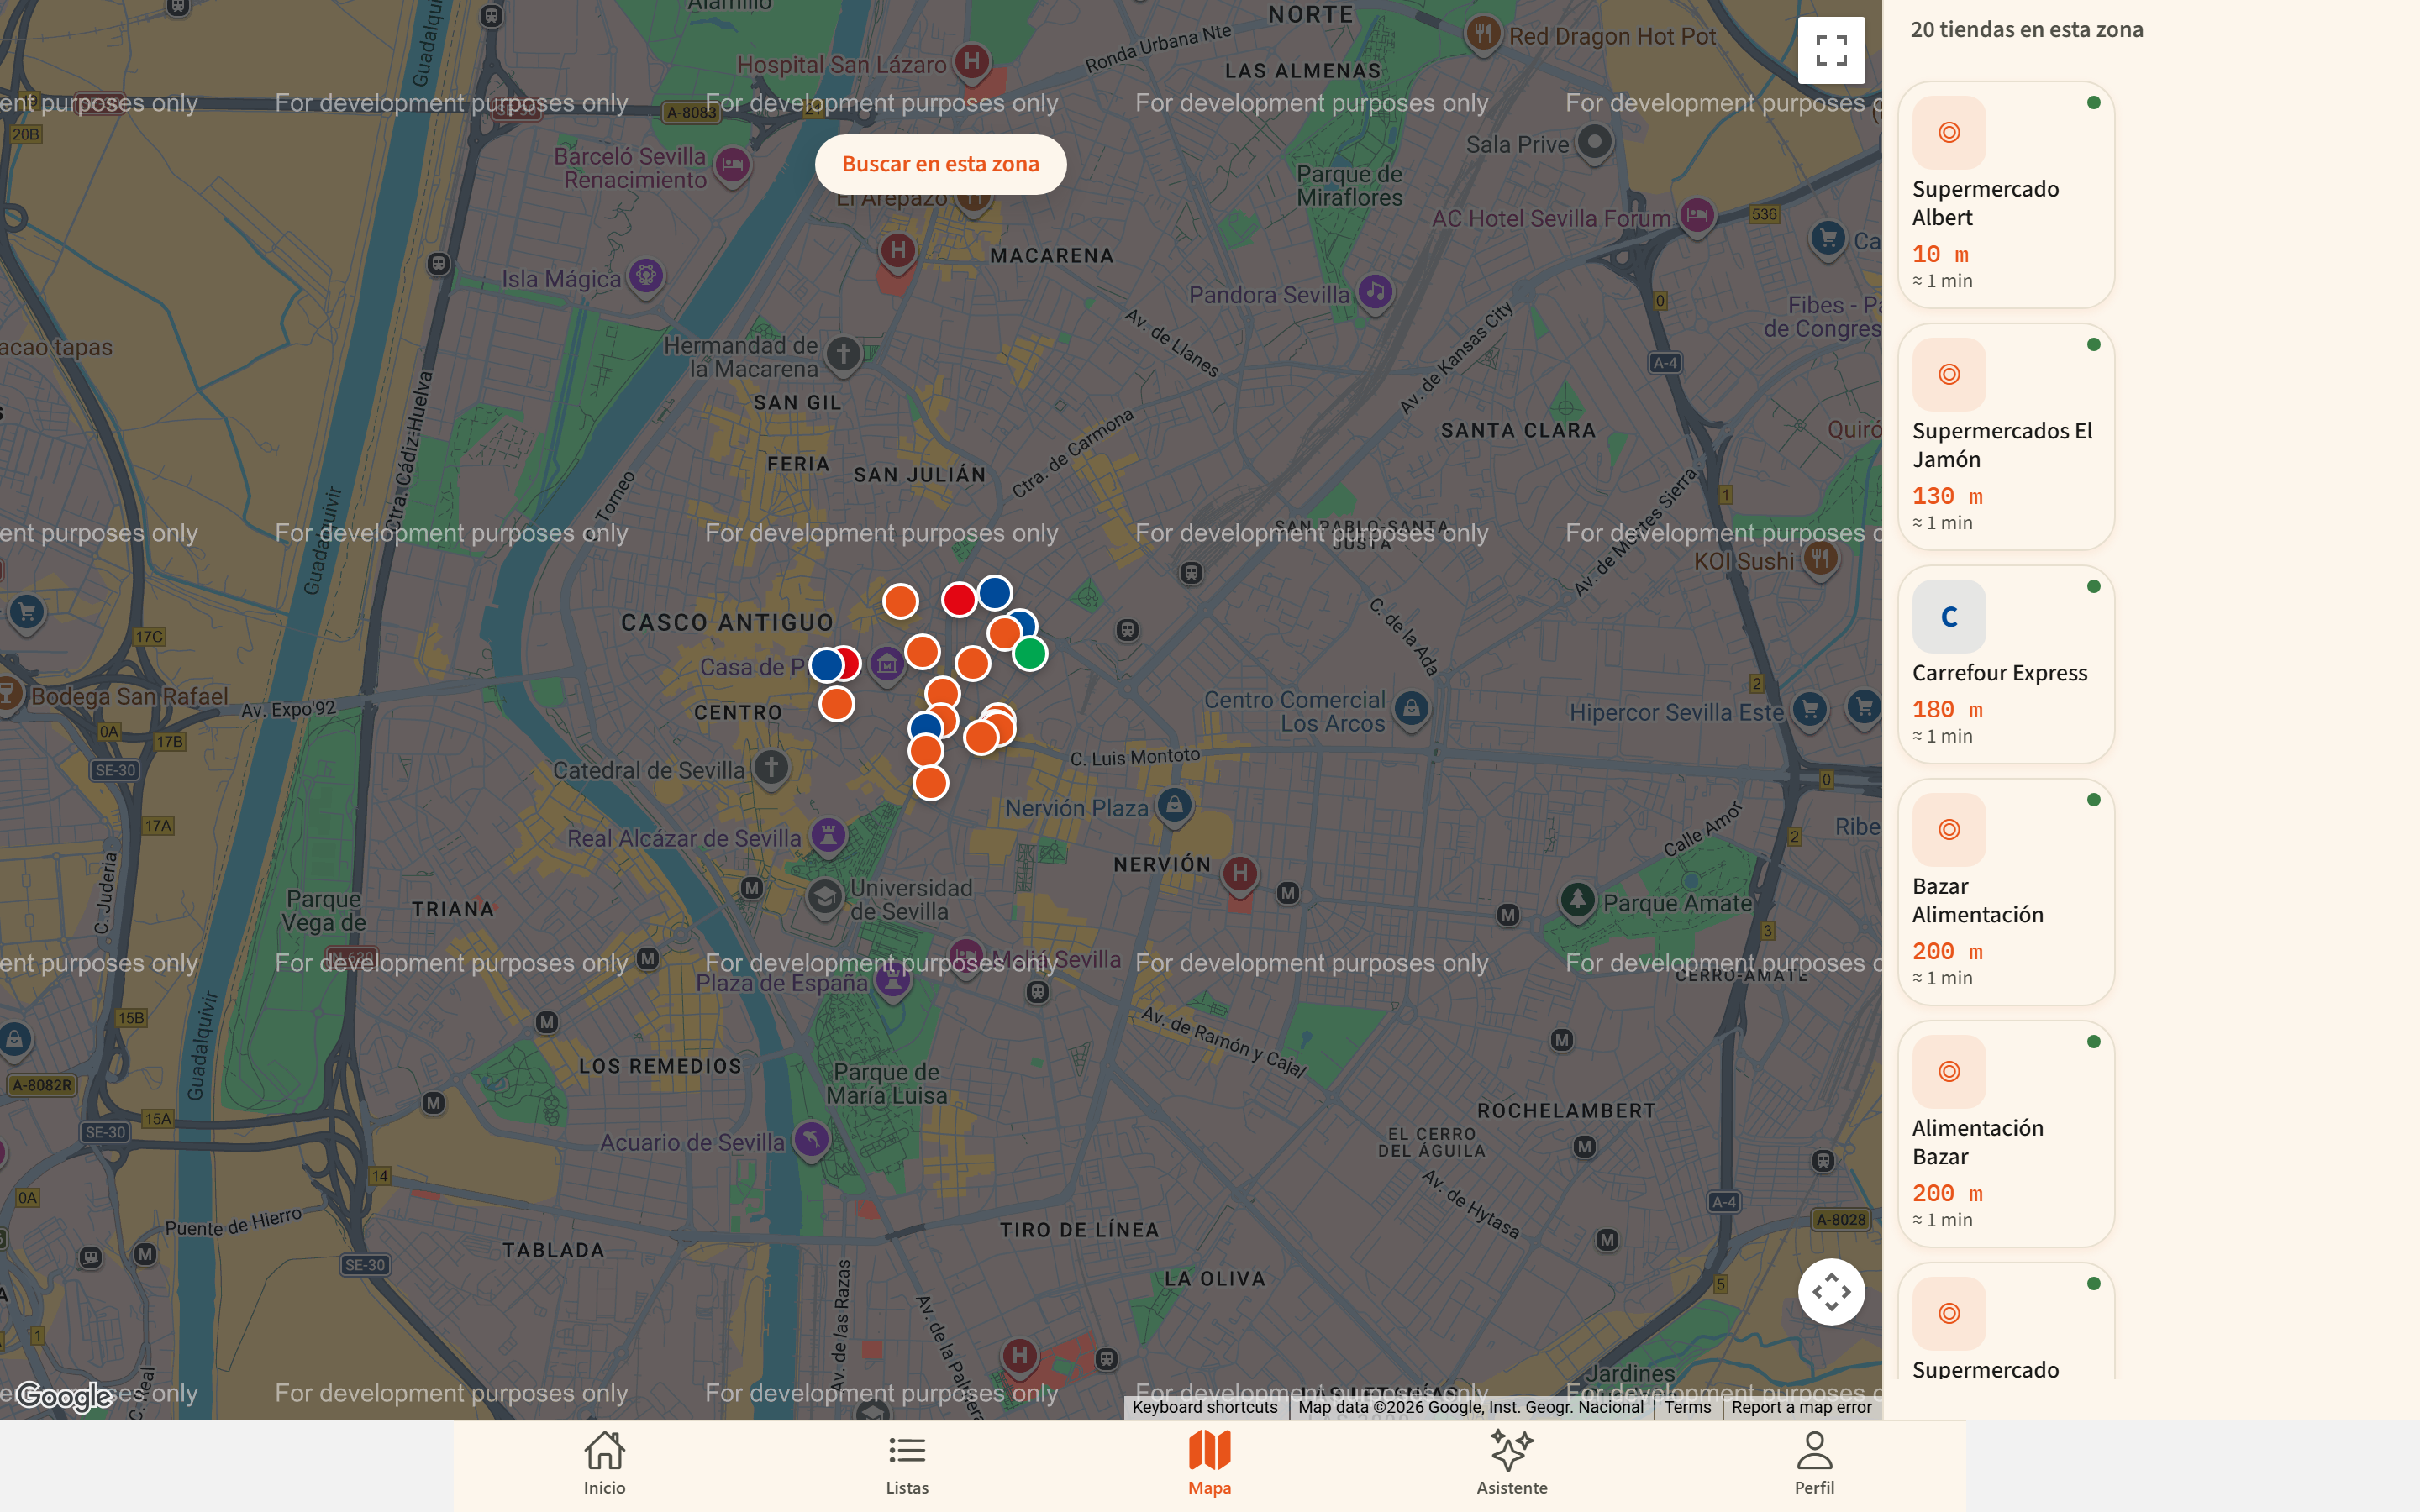
\includegraphics[width=0.46\textwidth]{diagramas/capturas/web-mapa.png}
\hfill
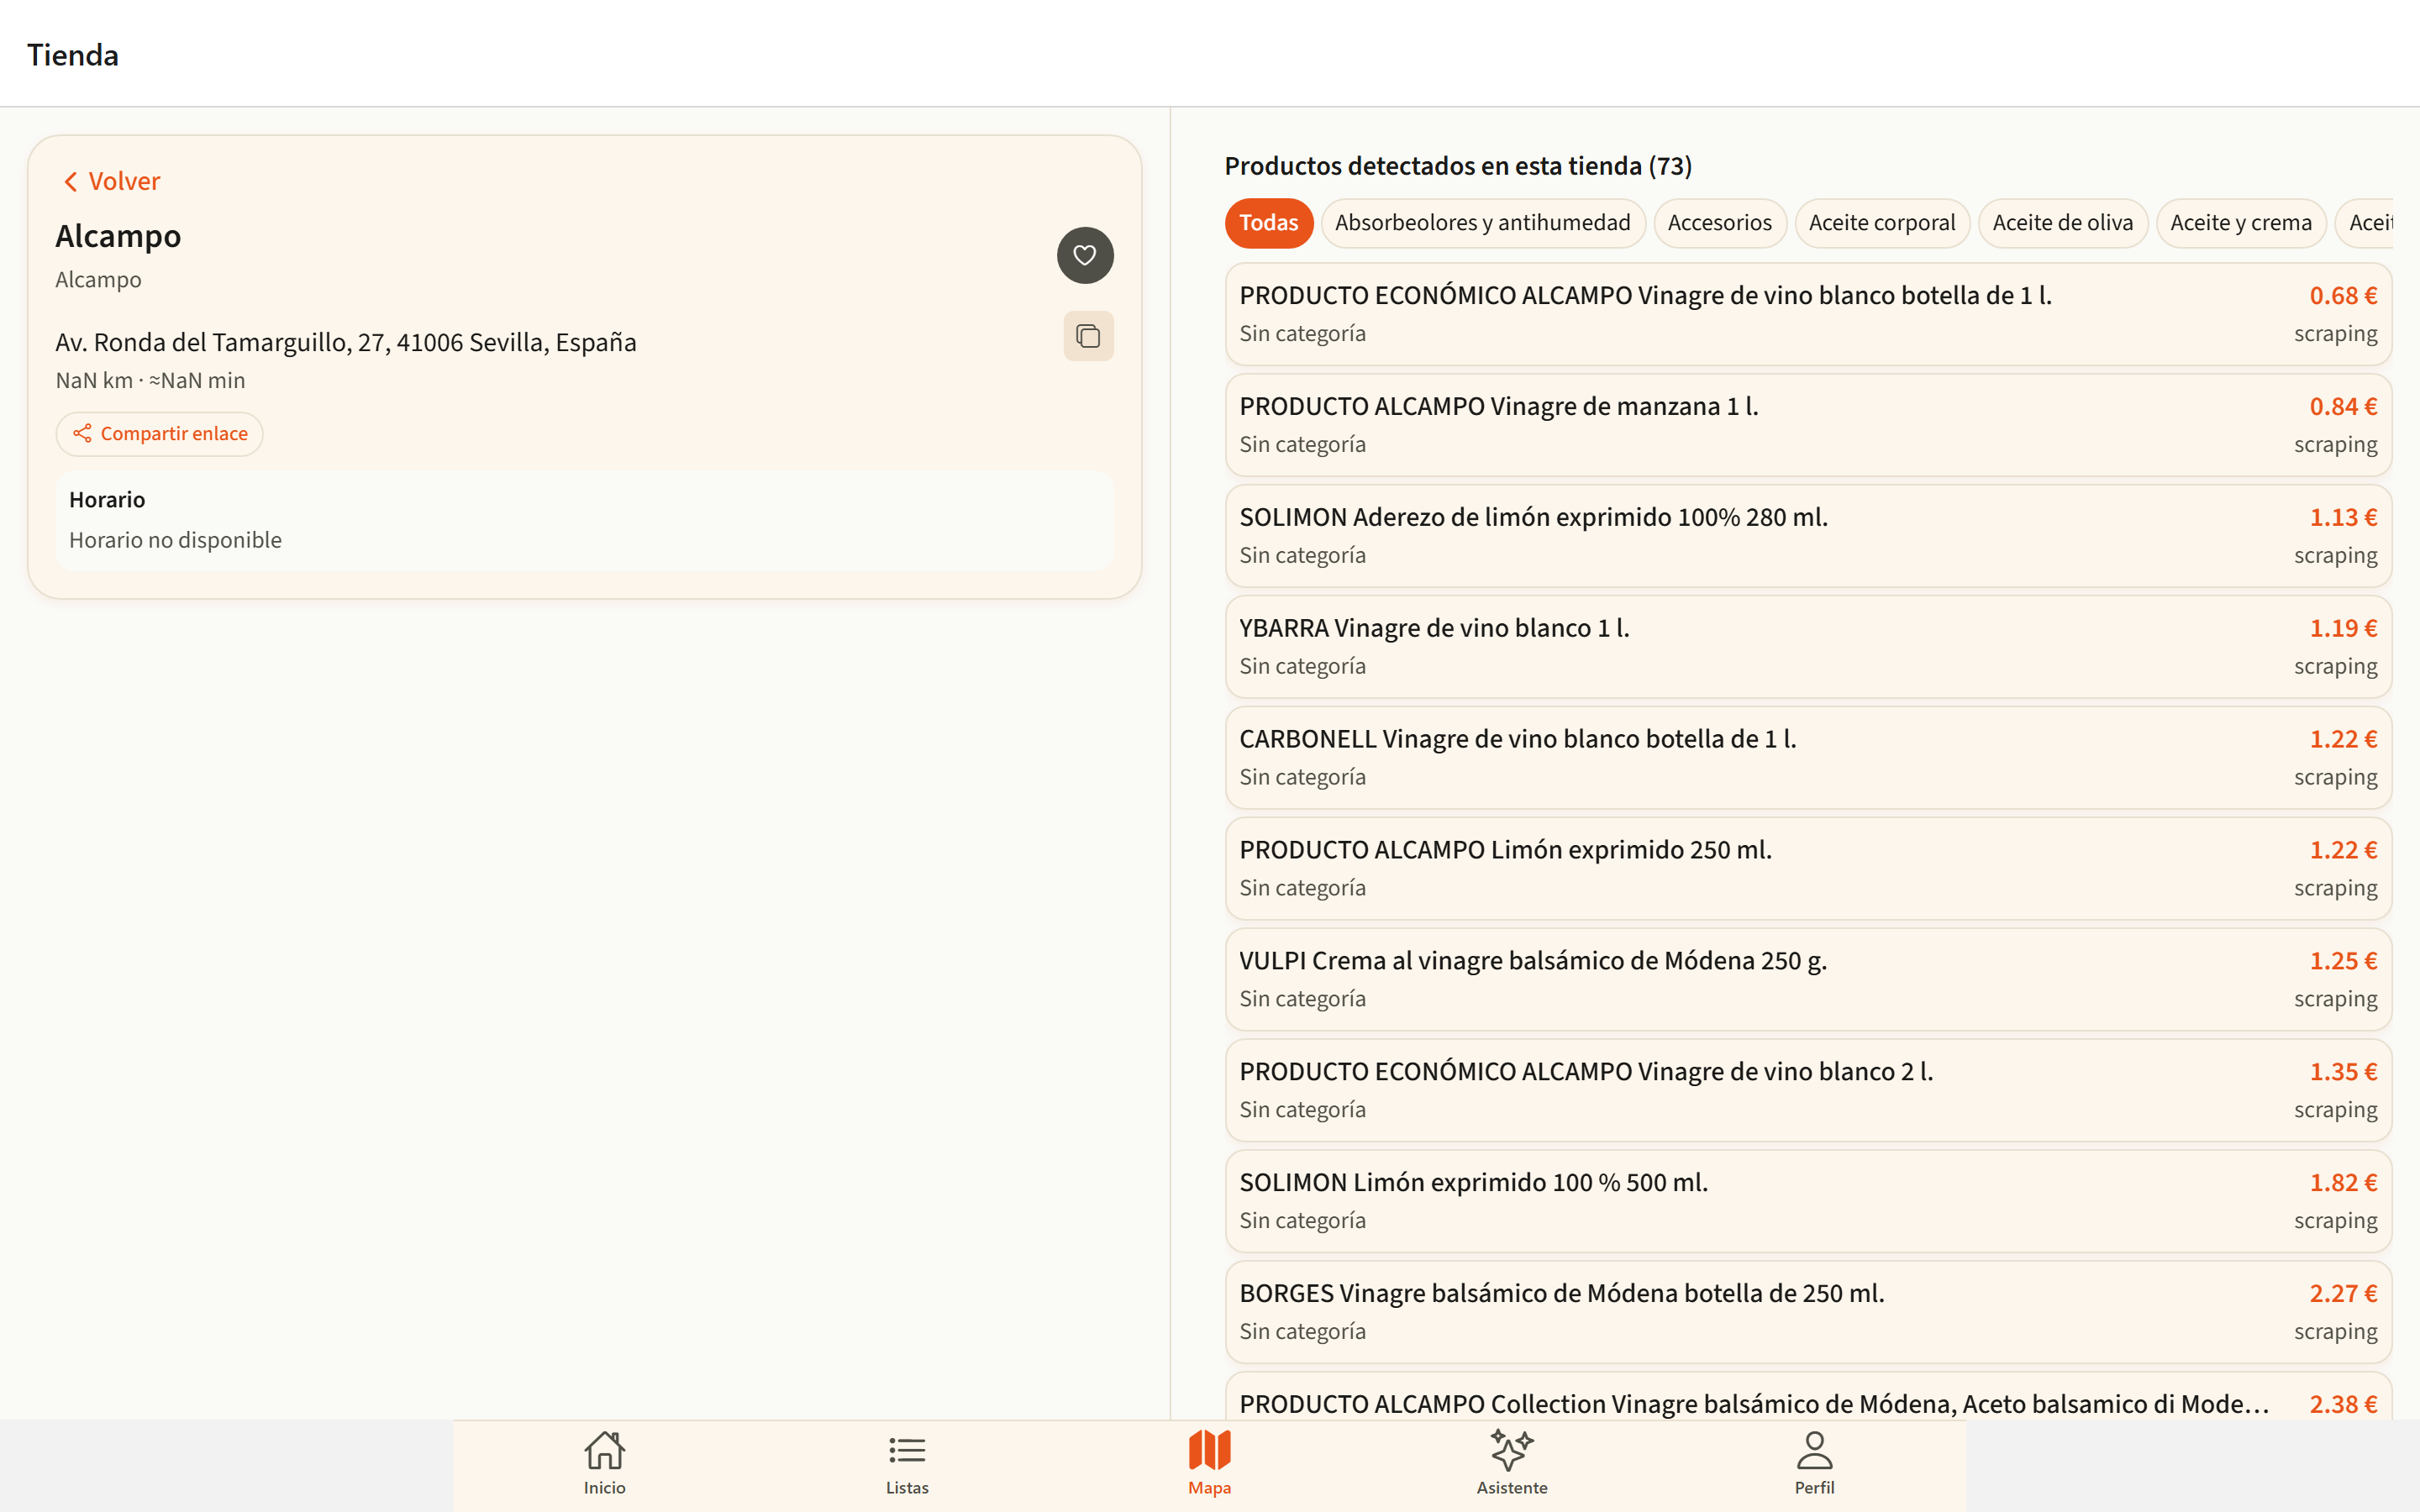
\includegraphics[width=0.46\textwidth]{diagramas/capturas/web-tienda-perfil.png}
\caption{Web --- Mapa con panel de tiendas anclado a la derecha (izquierda) y perfil de tienda a
dos columnas (derecha)}
\label{fig:cap-web-mapa-tienda}
\end{figure}

\clearpage

\begin{figure}[htbp]
\centering
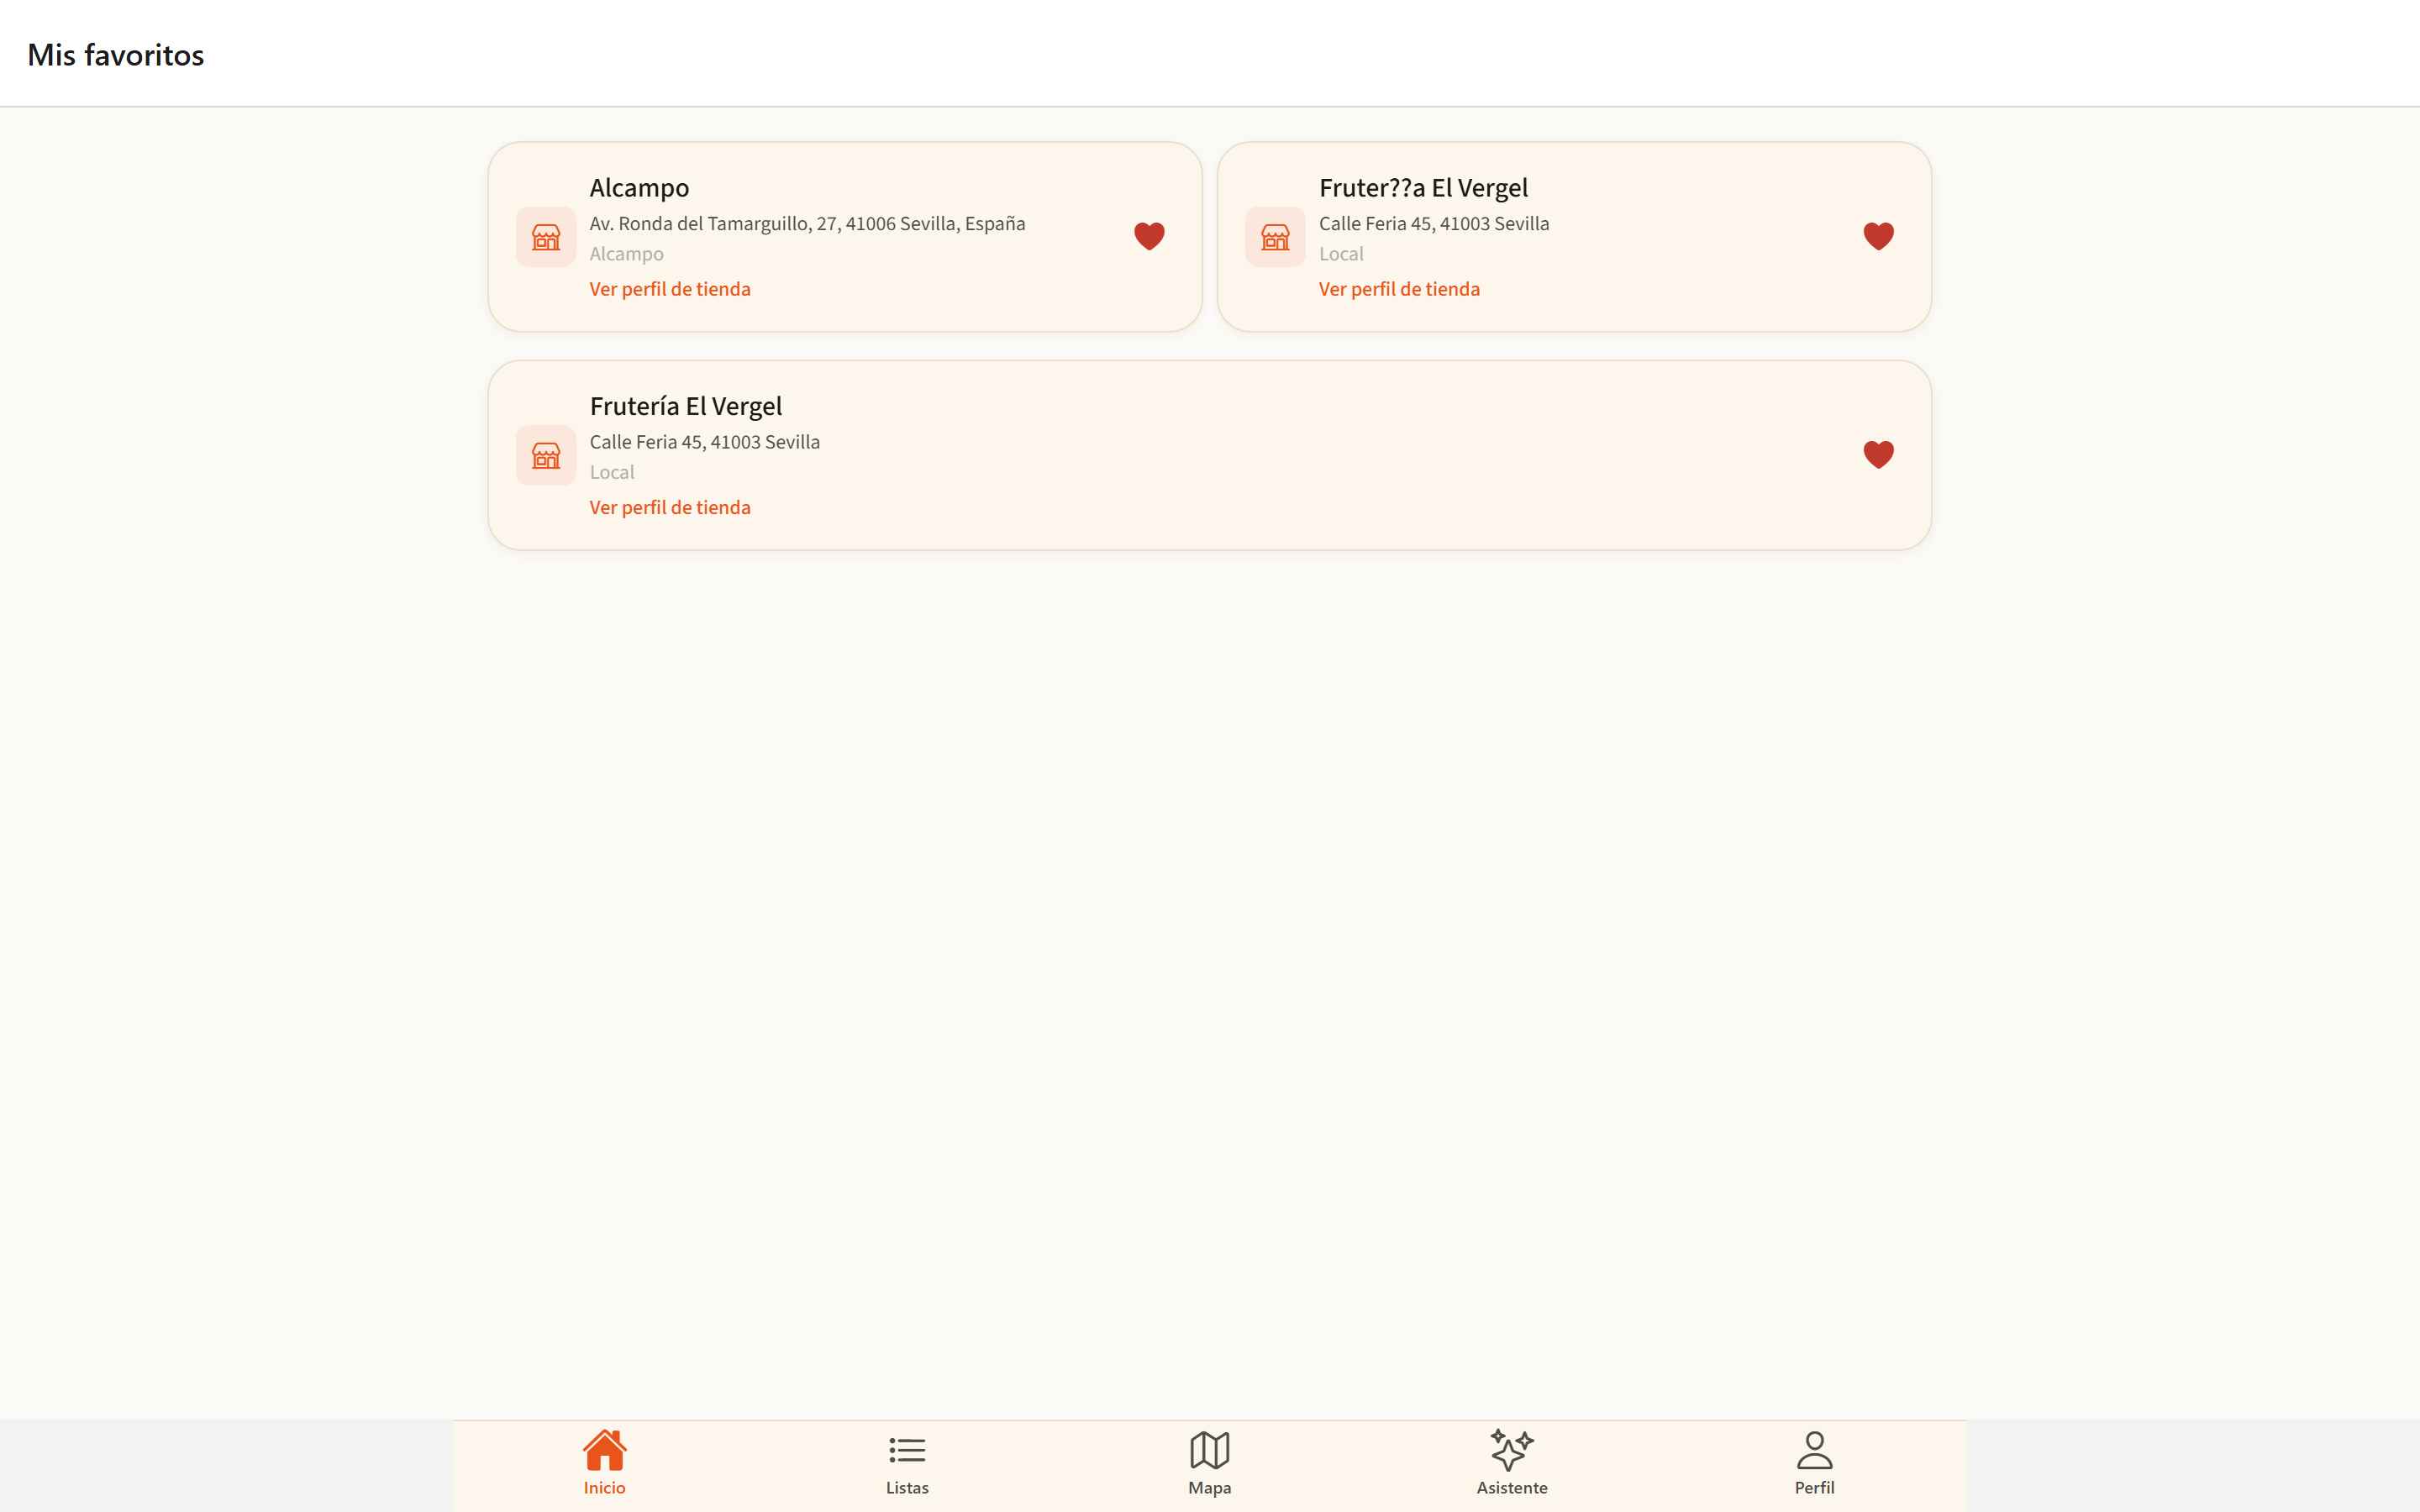
\includegraphics[width=0.46\textwidth]{diagramas/capturas/web-favoritas.png}
\hfill
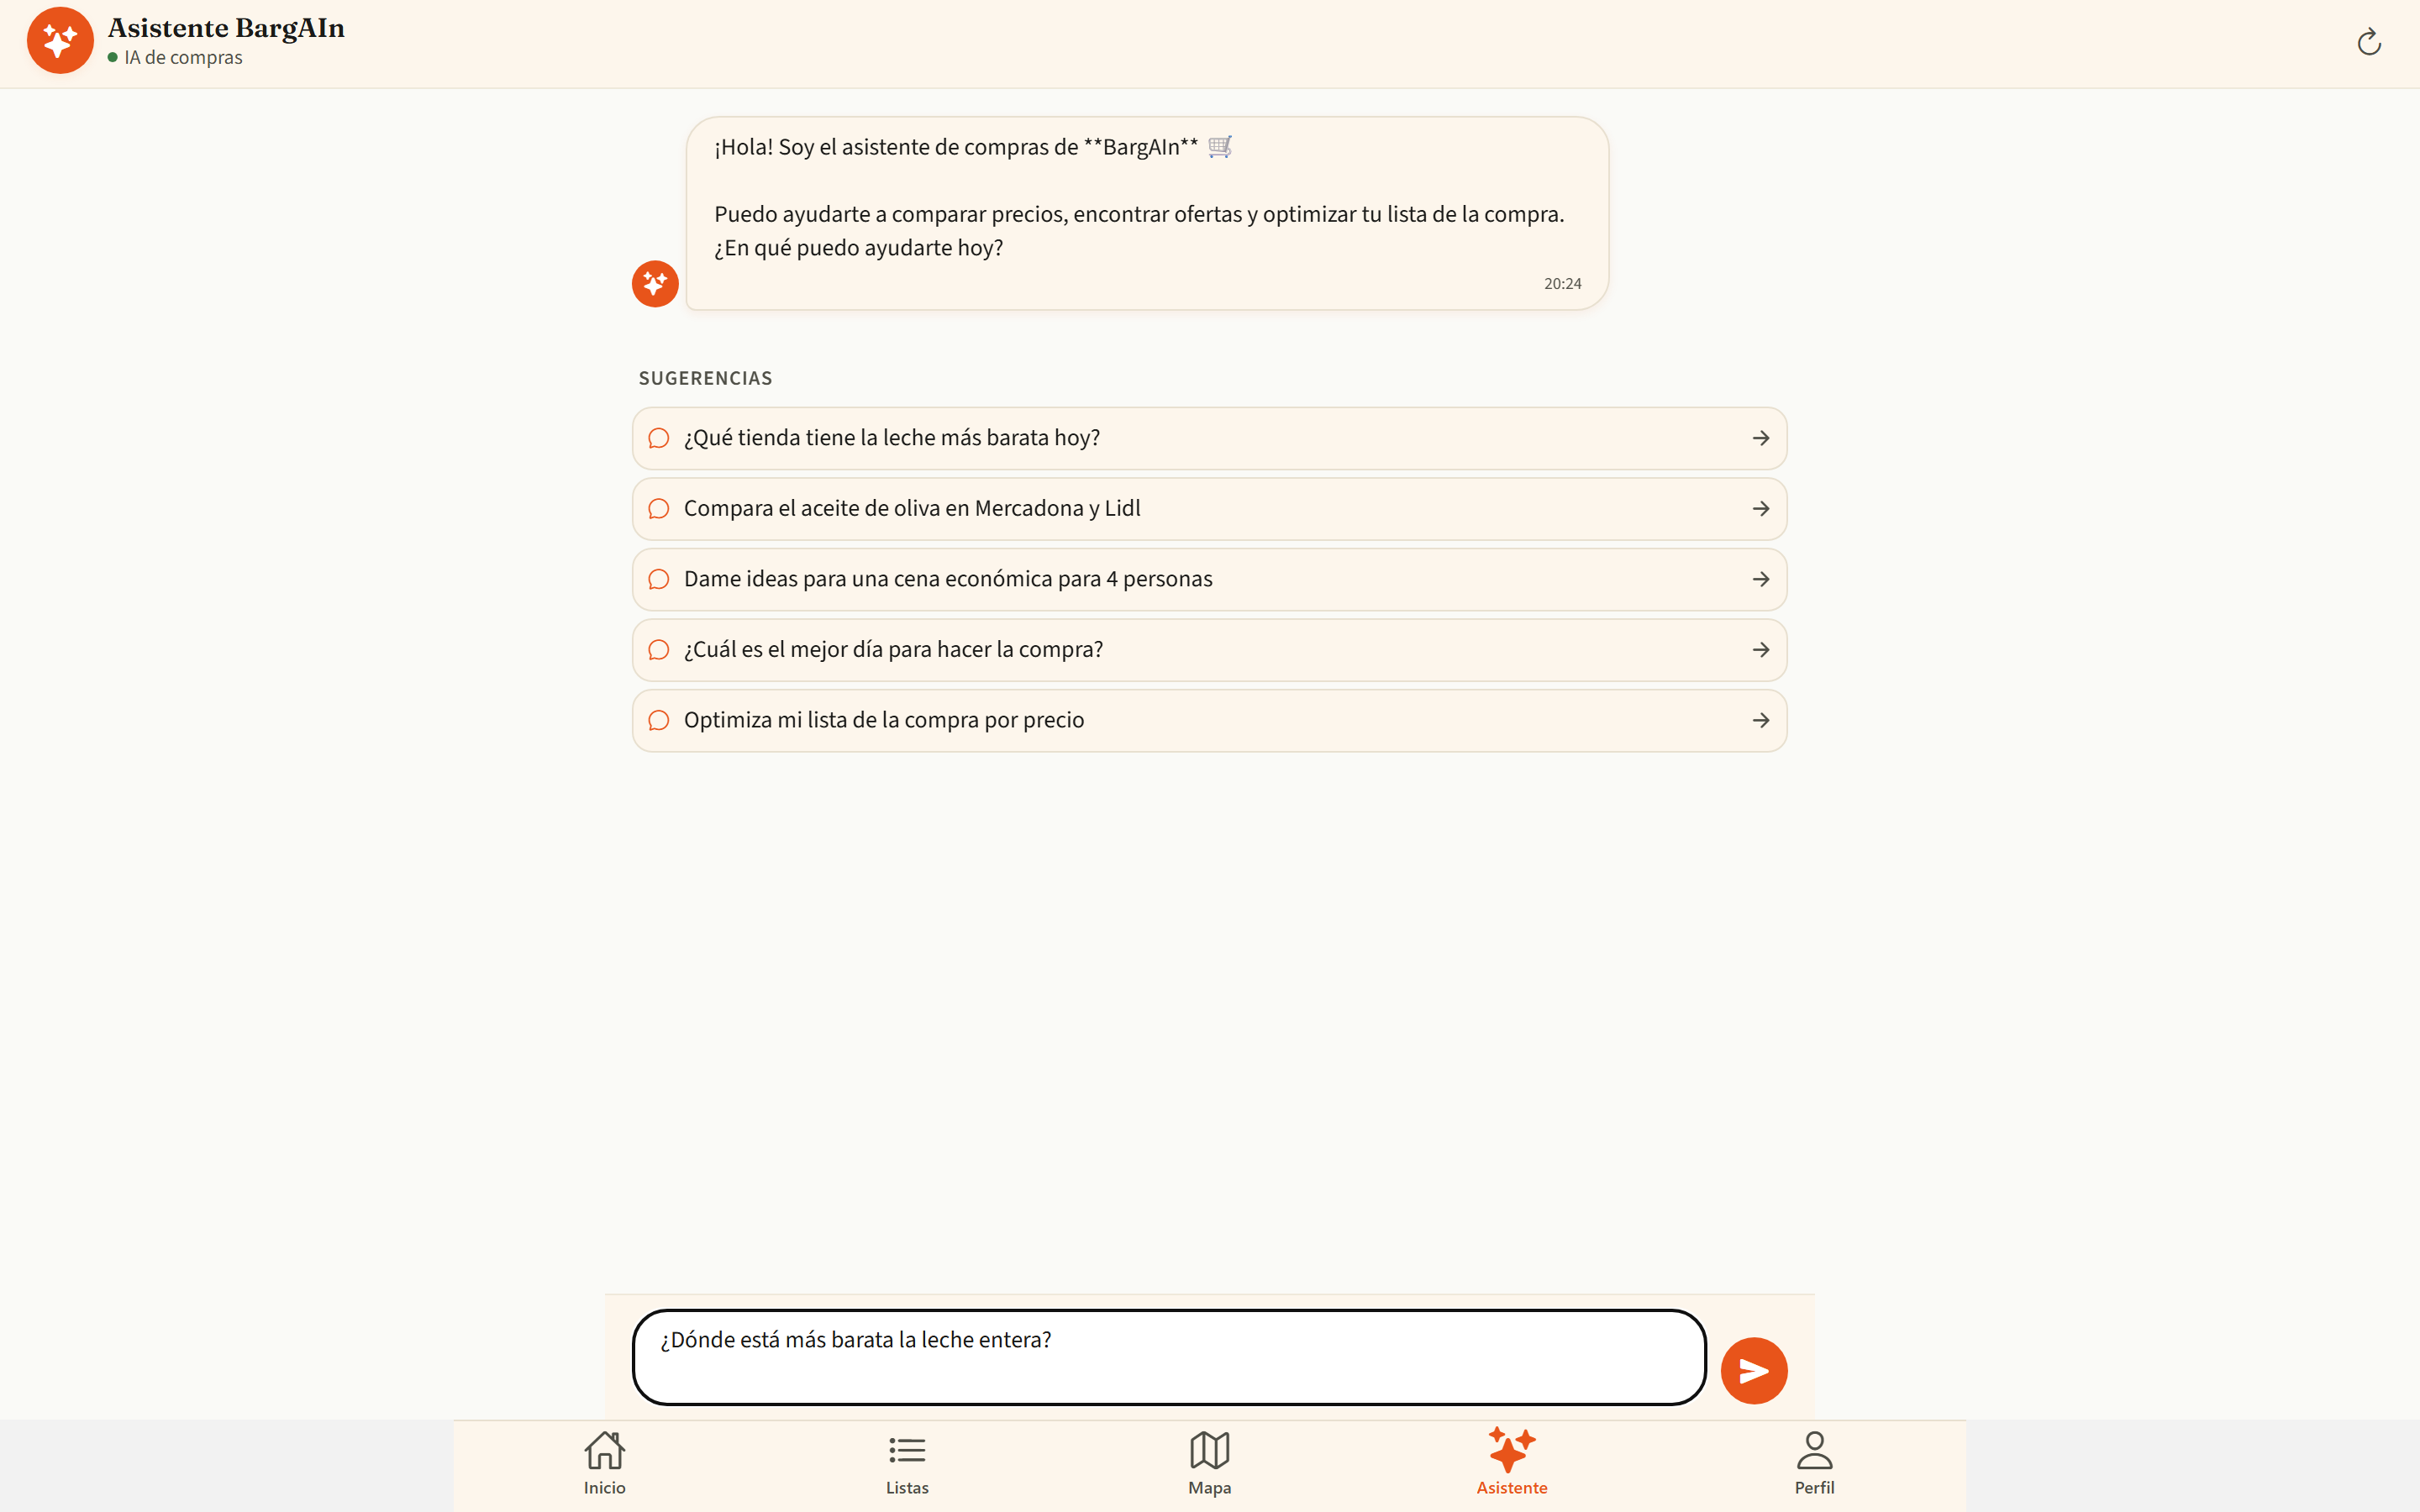
\includegraphics[width=0.46\textwidth]{diagramas/capturas/web-asistente.png}
\caption{Web --- Tiendas favoritas en rejilla (izquierda) y asistente centrado con copia por
mensaje (derecha)}
\label{fig:cap-web-favoritas-asistente}
\end{figure}

\begin{figure}[htbp]
\centering
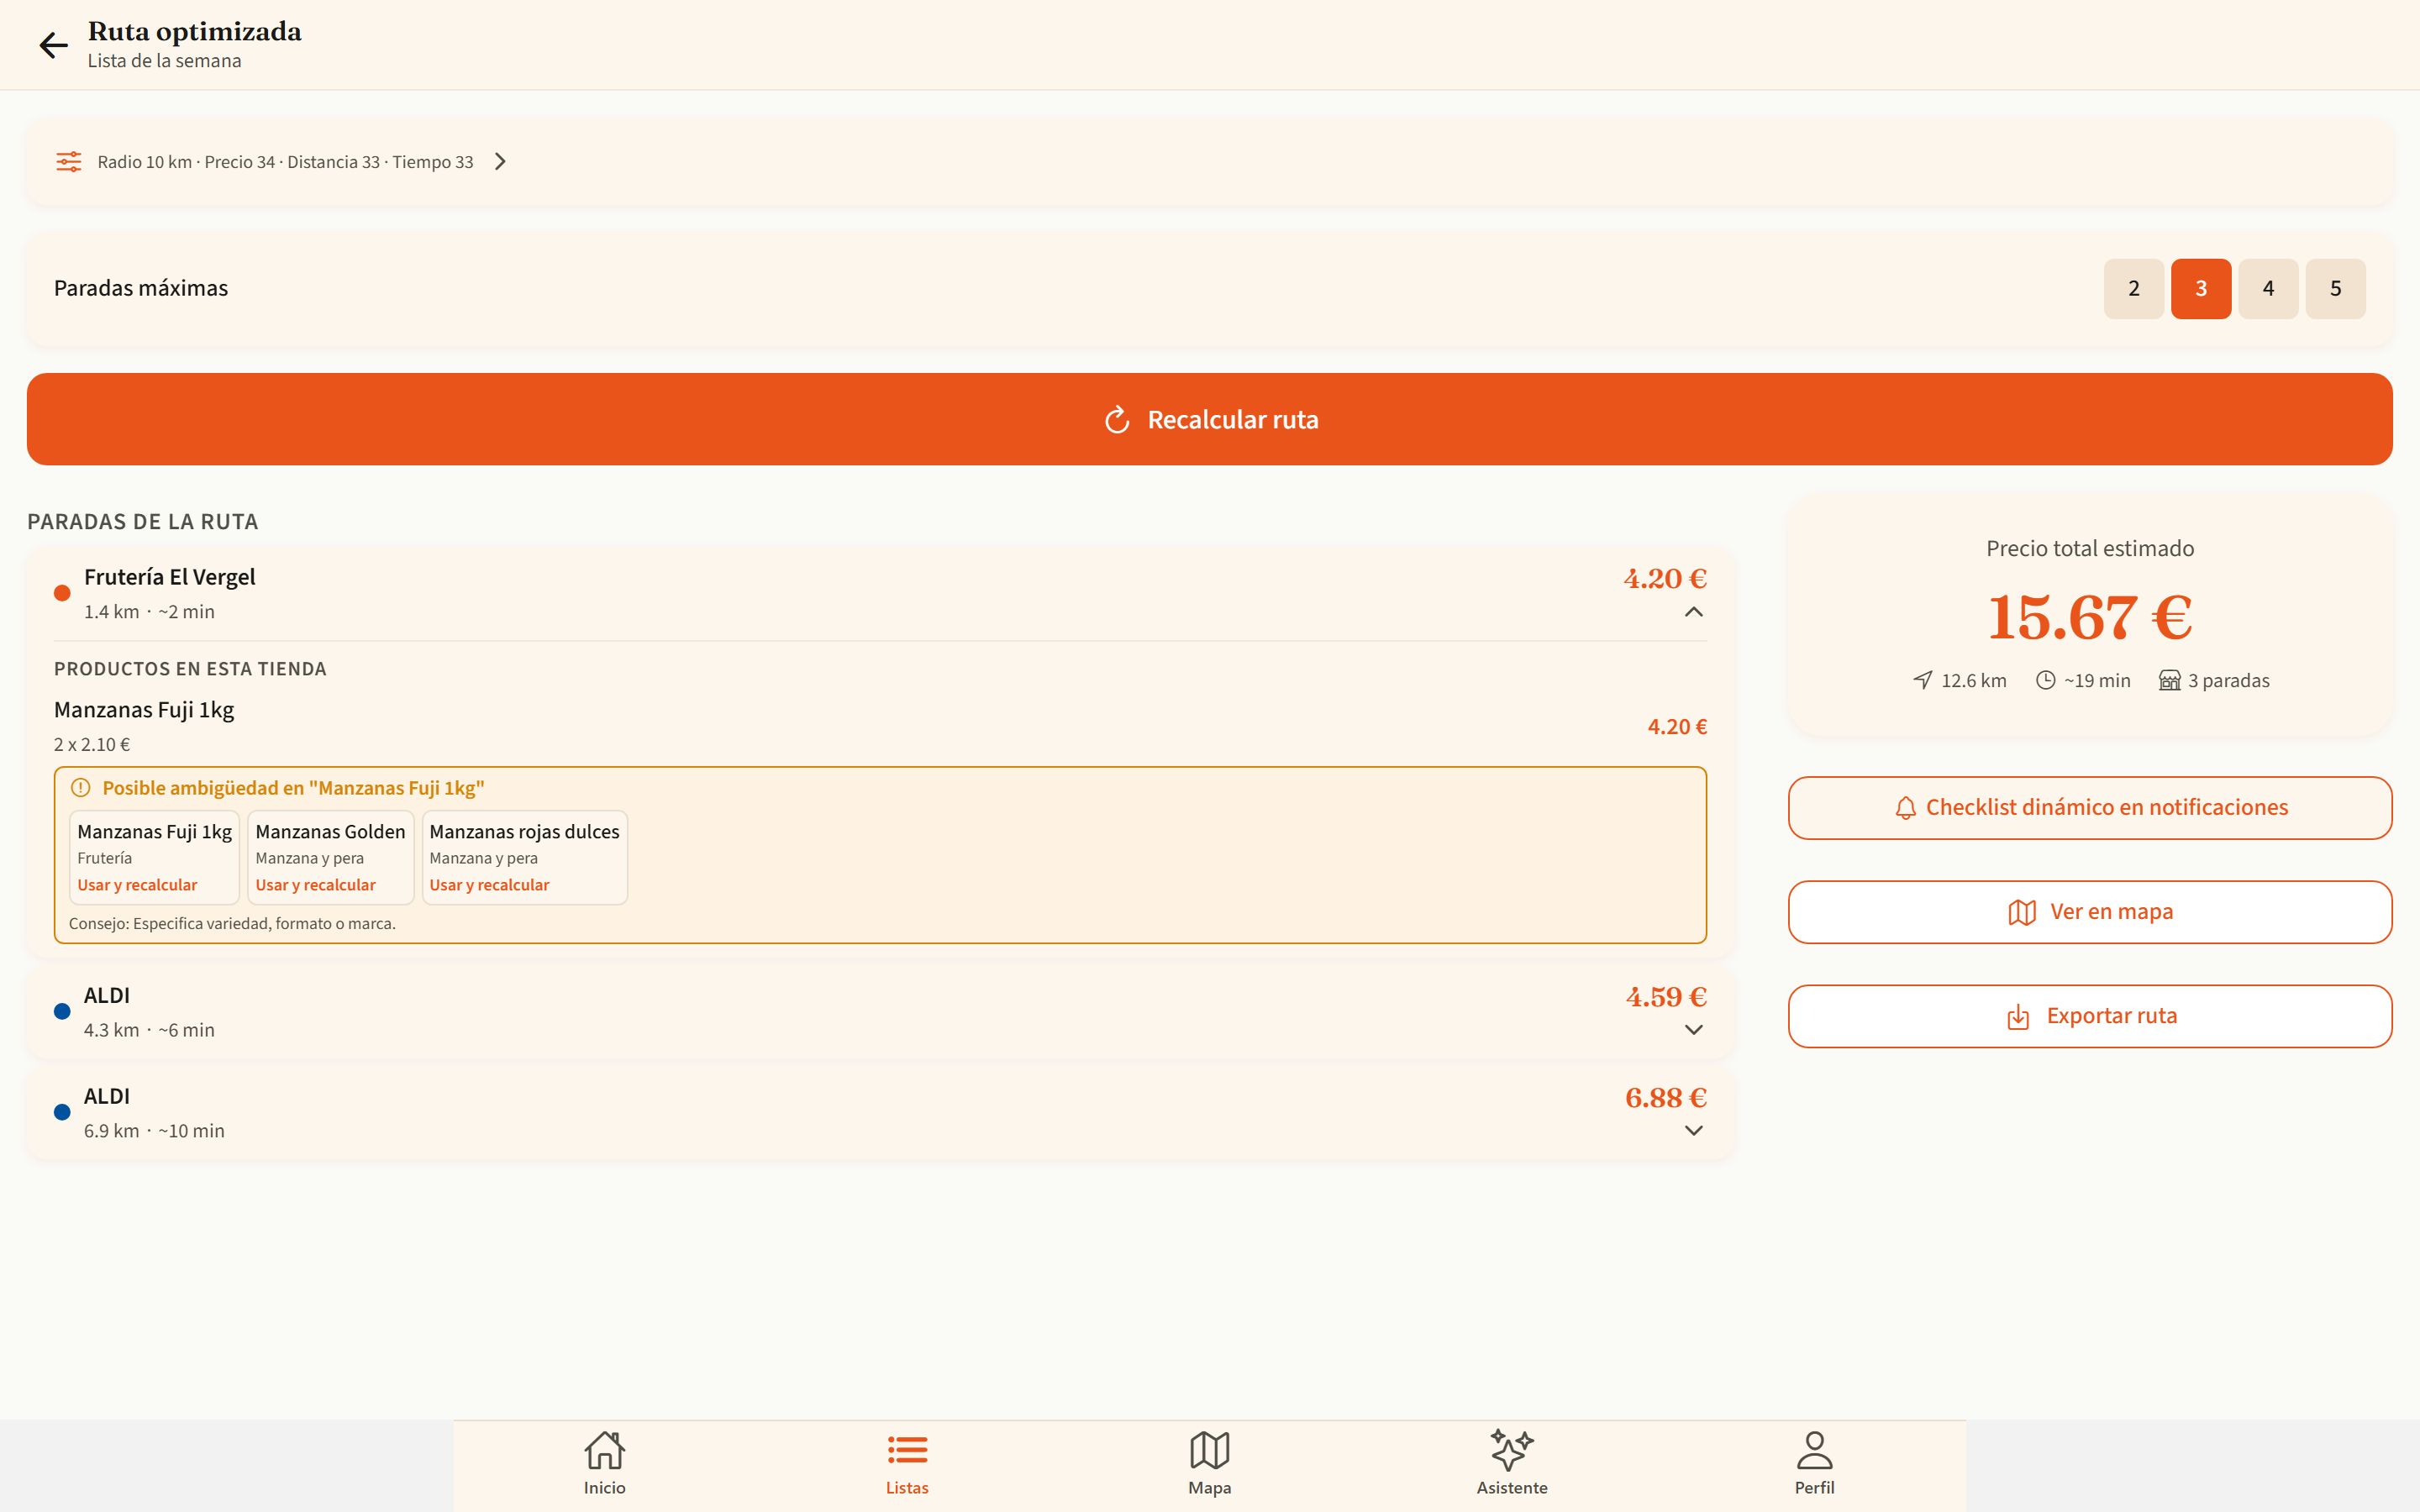
\includegraphics[width=0.46\textwidth]{diagramas/capturas/web-ruta.png}
\hfill
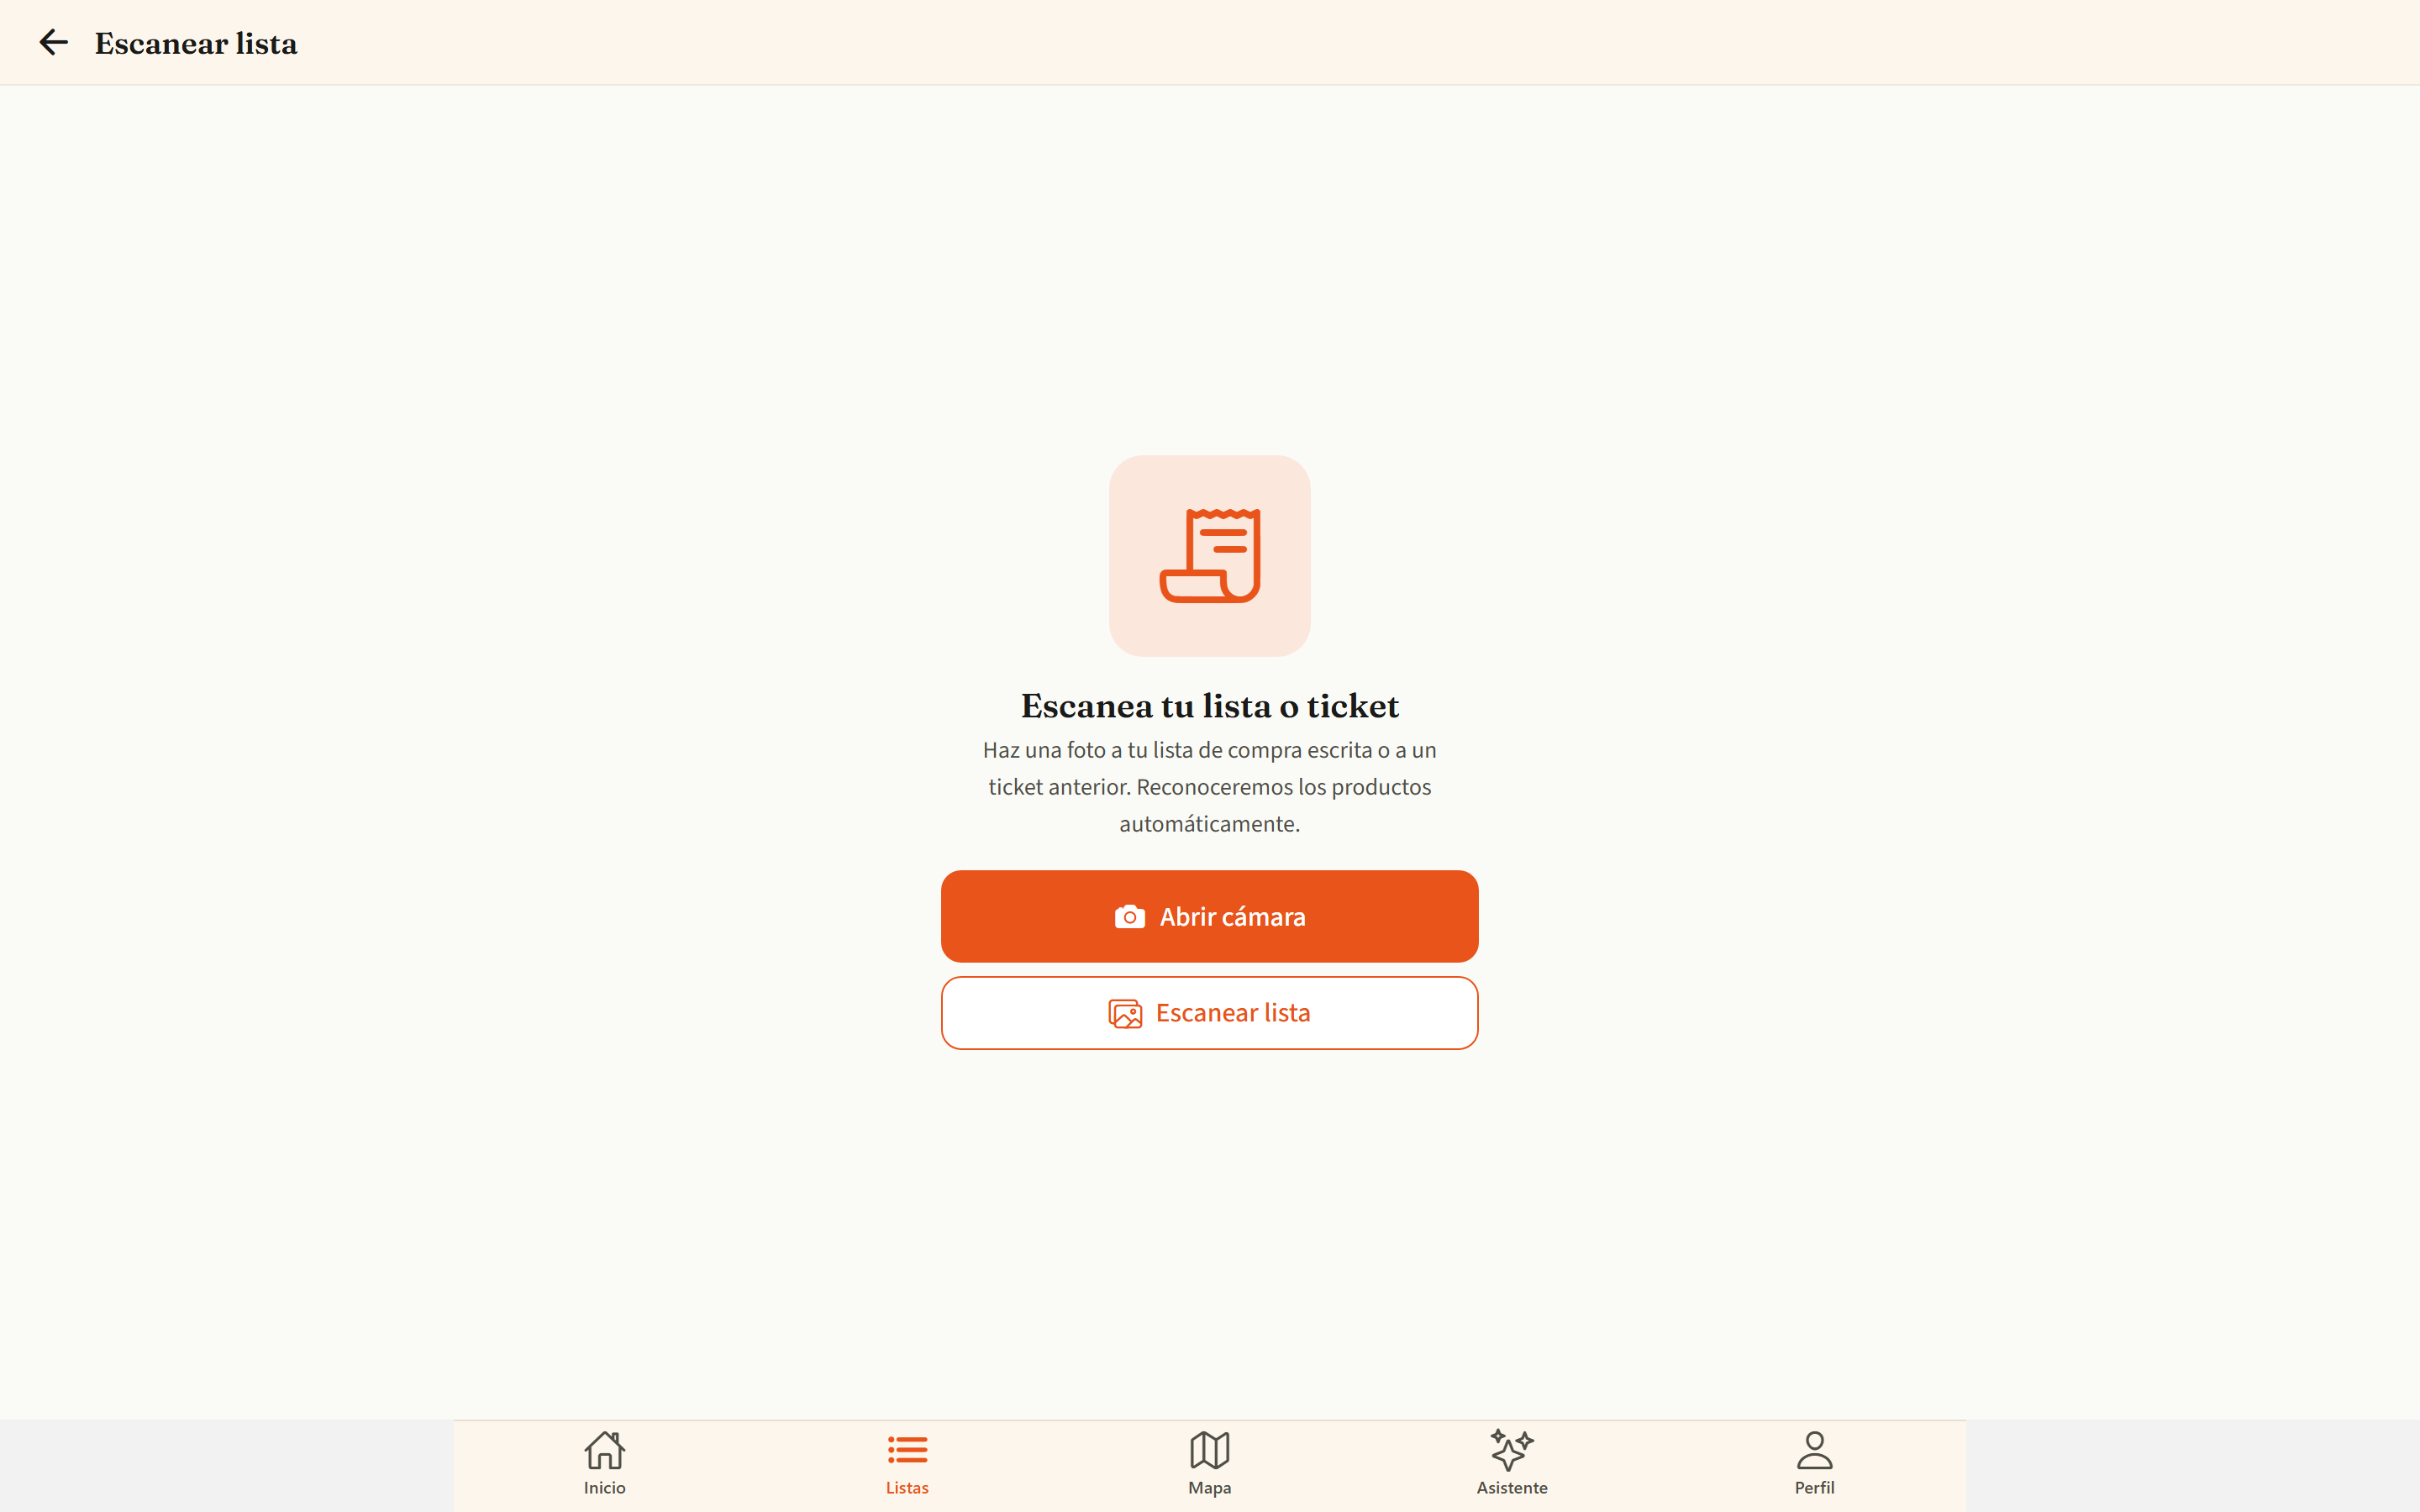
\includegraphics[width=0.46\textwidth]{diagramas/capturas/web-ocr.png}
\caption{Web --- Ruta optimizada con exportaci\'on (izquierda) y m\'odulo OCR centrado (derecha)}
\label{fig:cap-web-ruta-ocr}
\end{figure}

\begin{figure}[htbp]
\centering
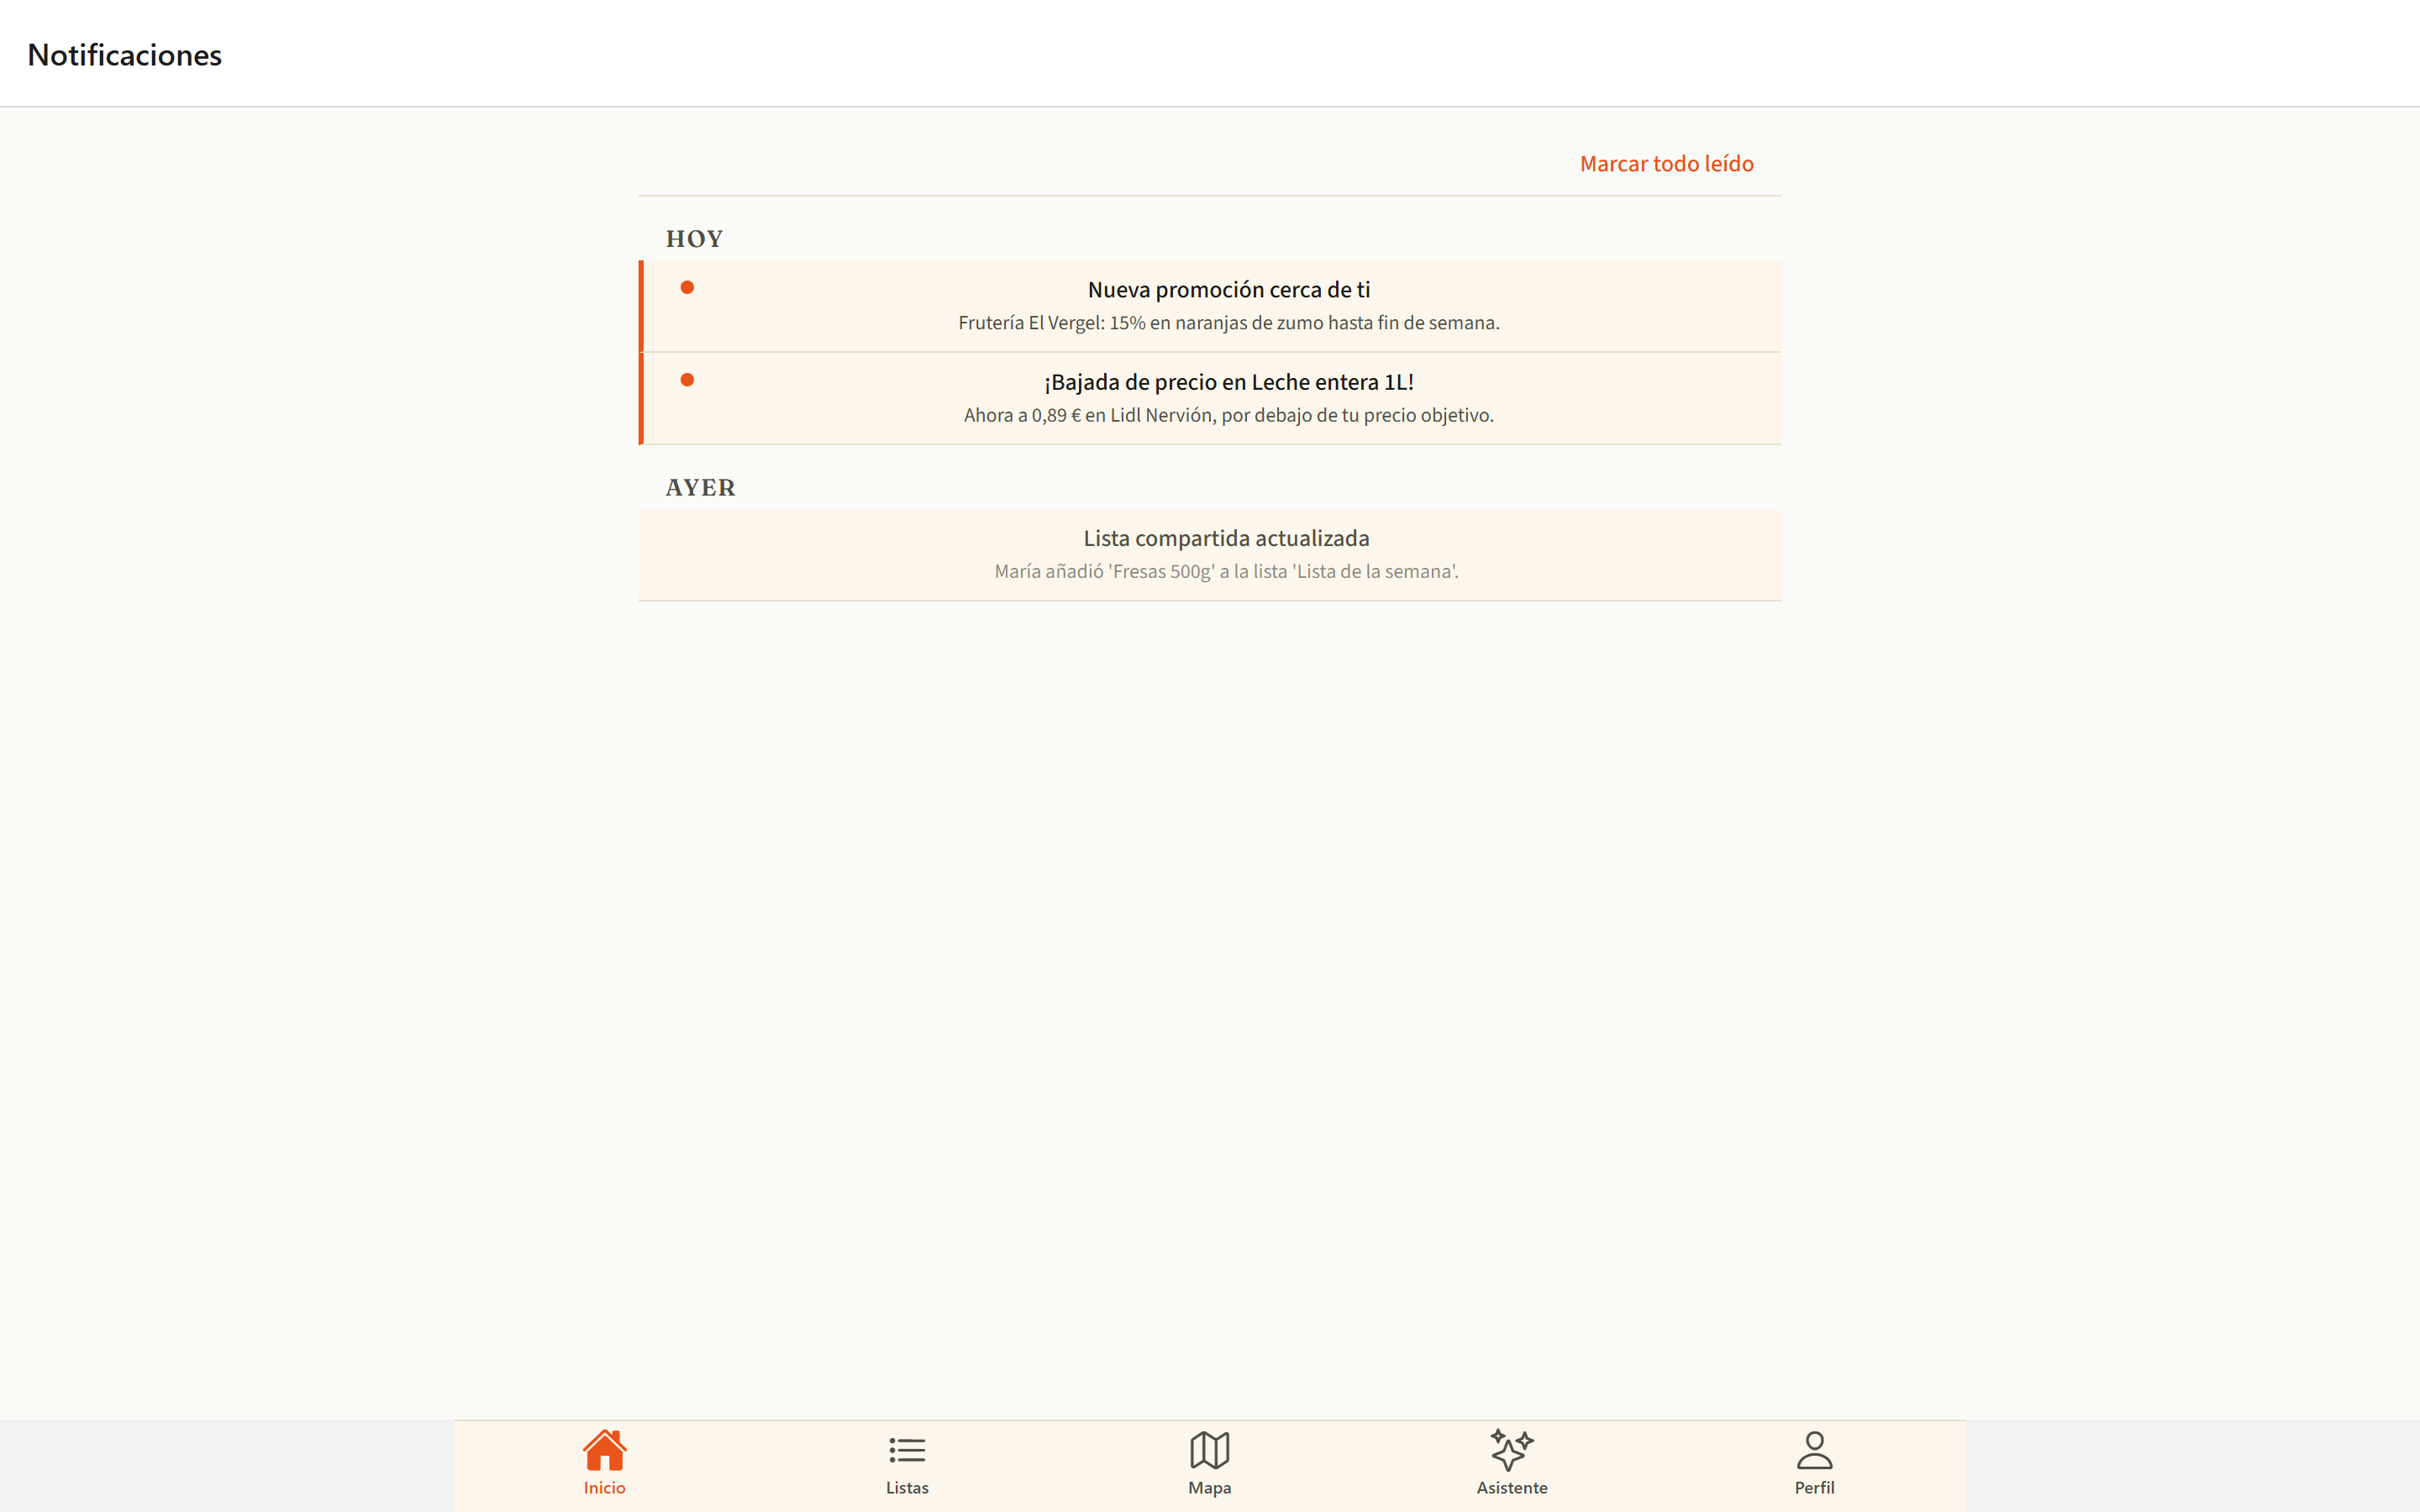
\includegraphics[width=0.46\textwidth]{diagramas/capturas/web-notificaciones.png}
\hfill
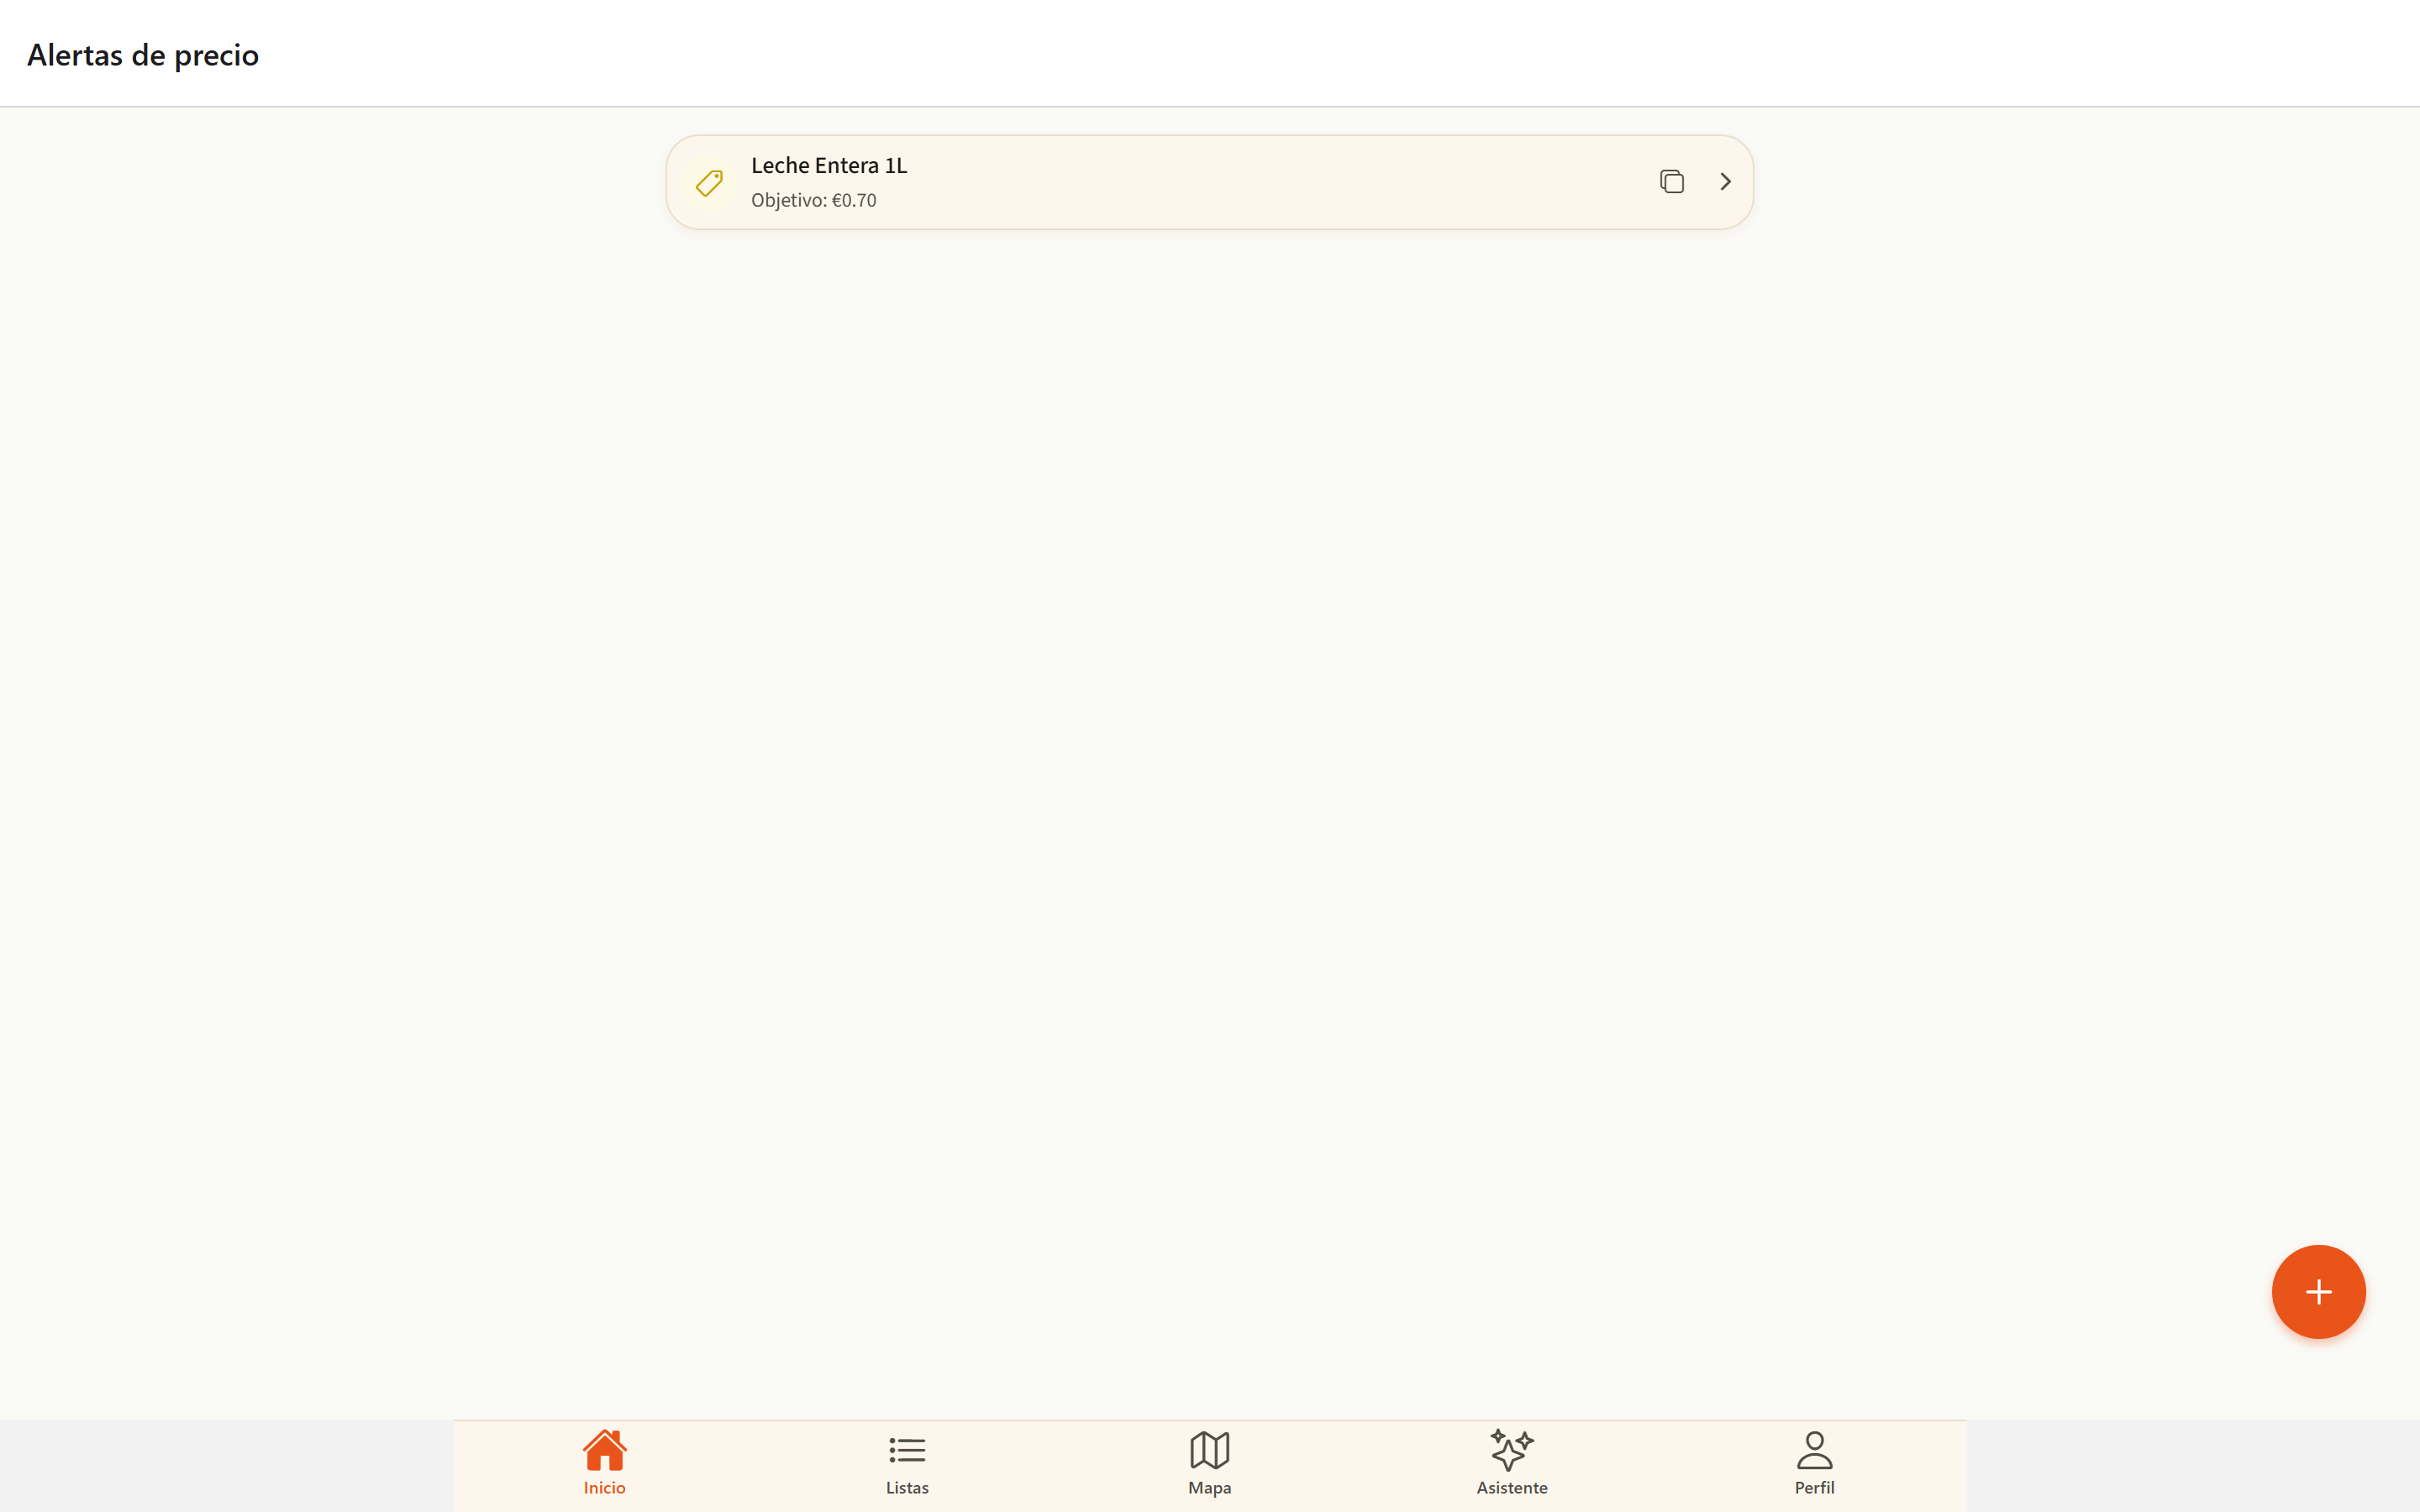
\includegraphics[width=0.46\textwidth]{diagramas/capturas/web-alertas.png}
\caption{Web --- Bandeja de notificaciones (izquierda) y alertas de precio (derecha) centradas}
\label{fig:cap-web-notif-alertas}
\end{figure}

\clearpage

\subsection{Portal web para PYMEs}\label{subsec:galeria-pyme}

\begin{figure}[htbp]
\centering
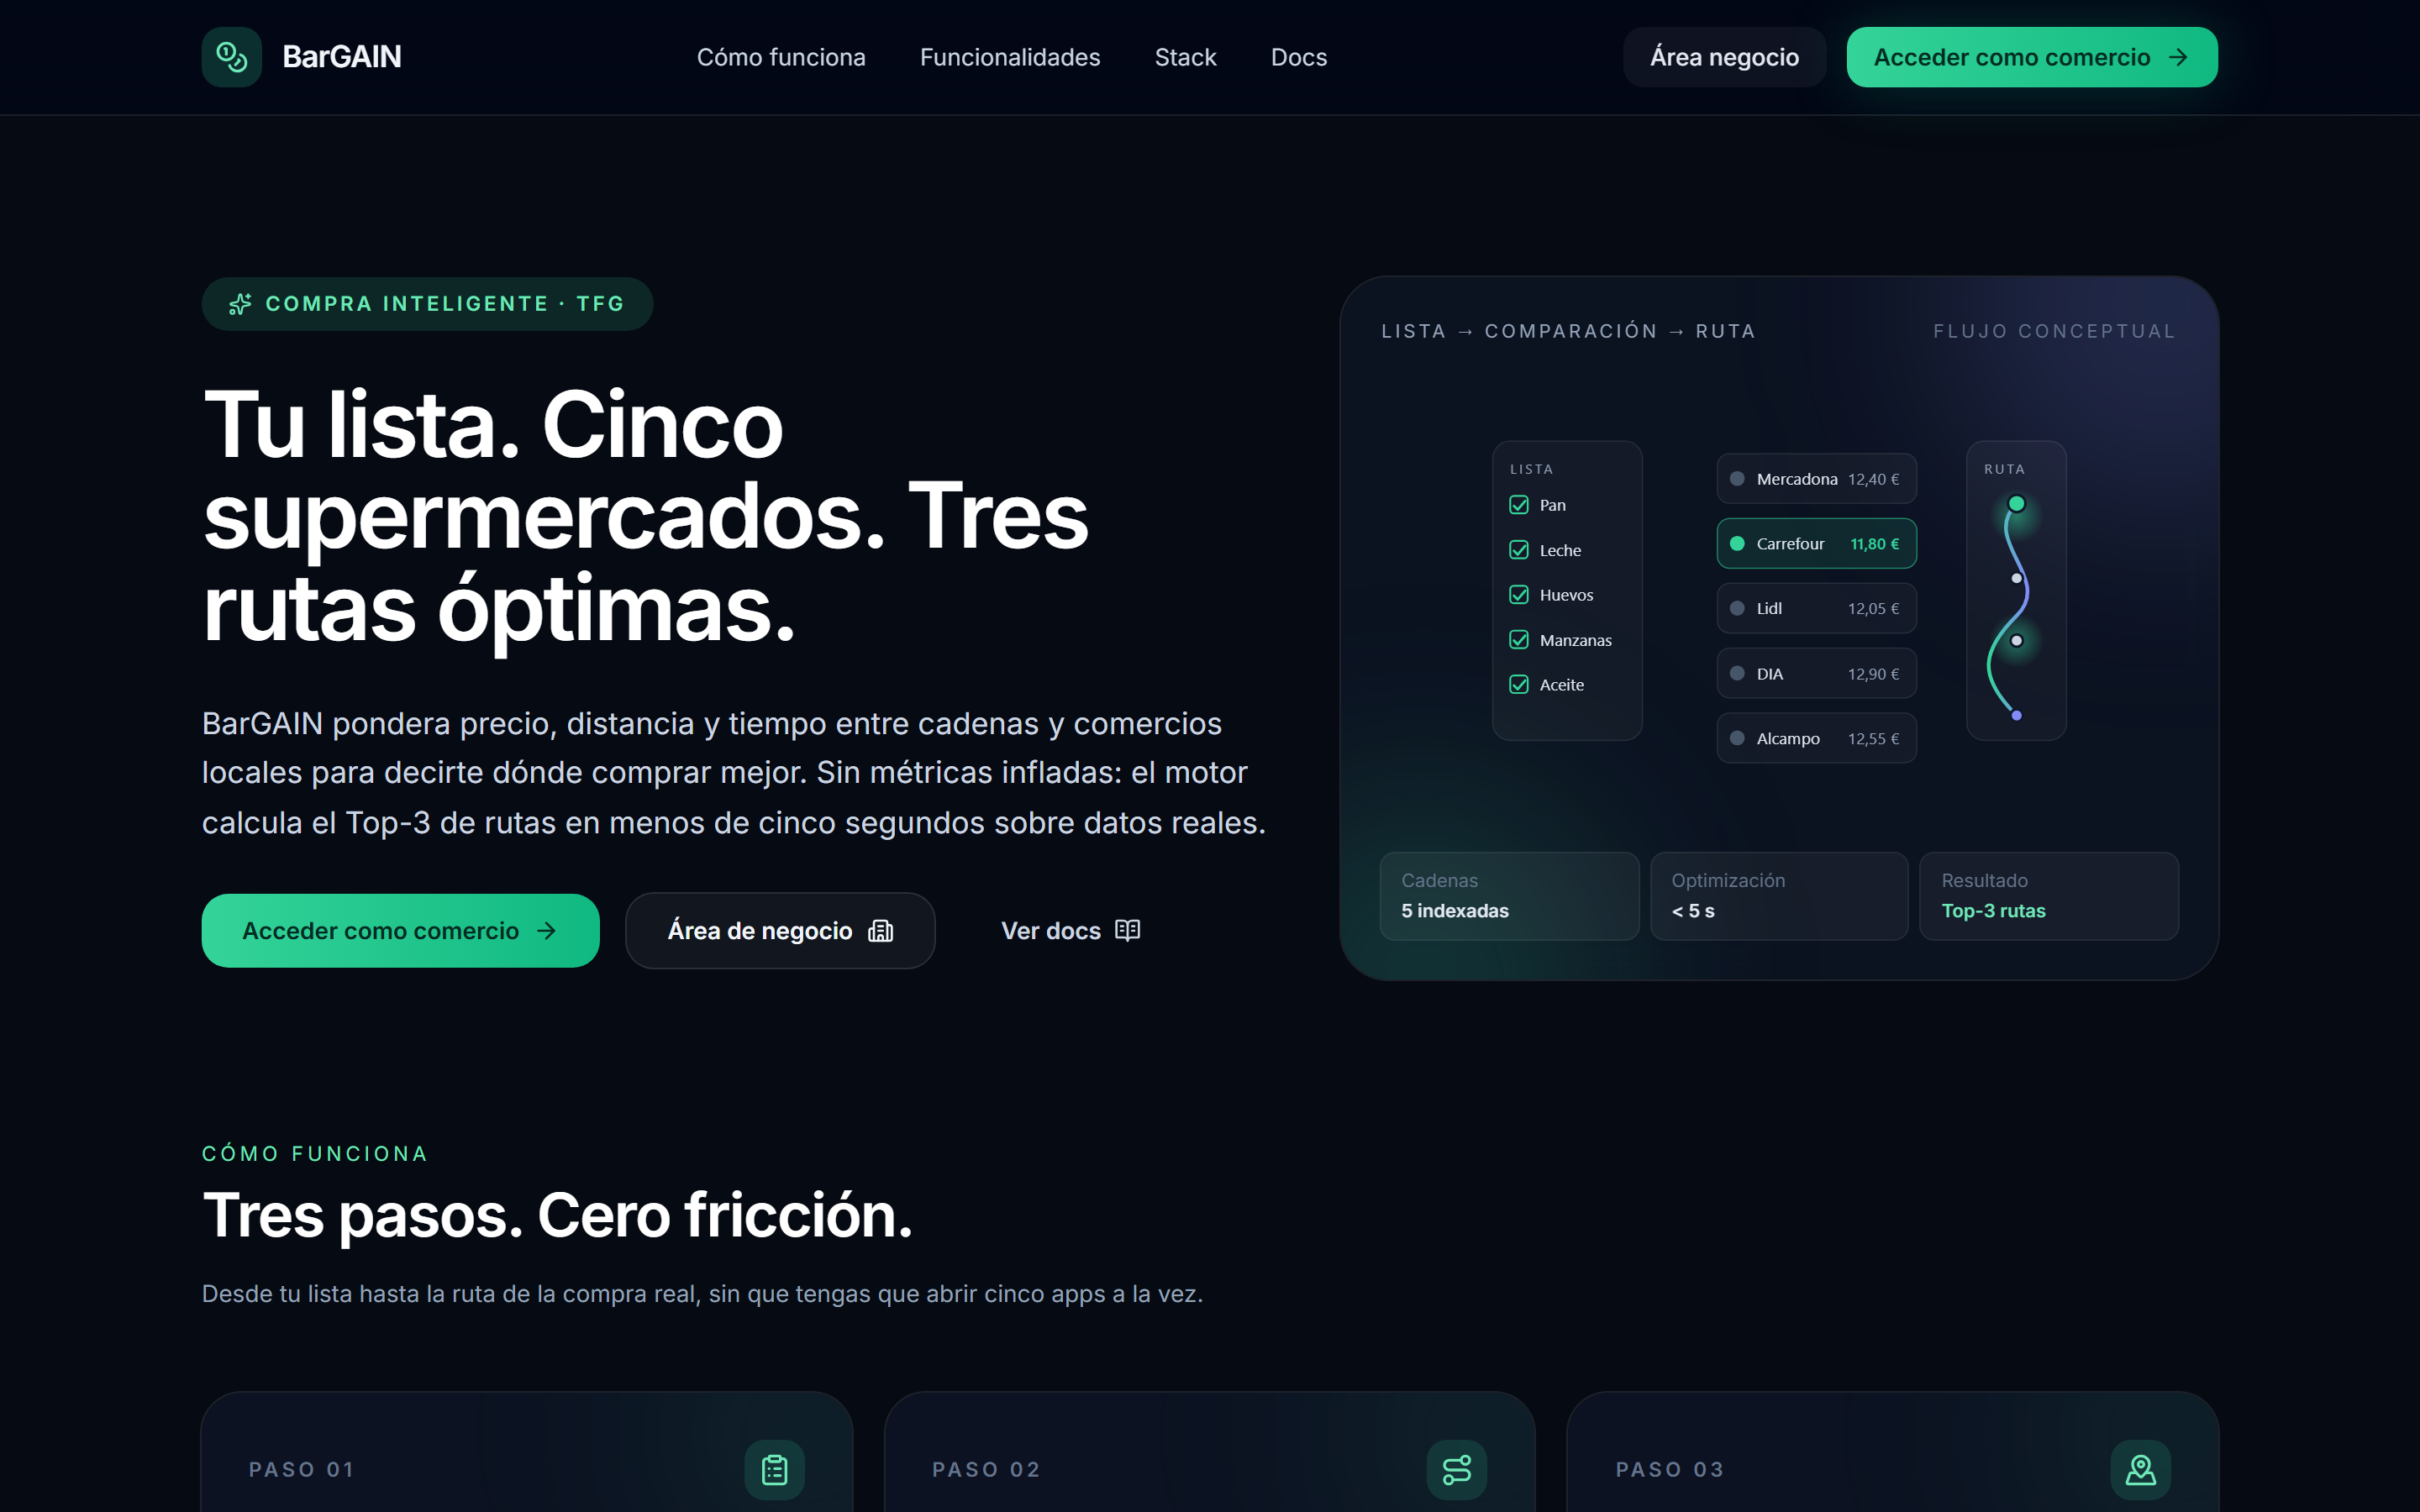
\includegraphics[width=0.85\textwidth]{diagramas/capturas/pyme-landing.png}
\caption{Portal PYME --- P\'agina de aterrizaje (\emph{landing})}
\label{fig:cap-pyme-landing}
\end{figure}

\begin{figure}[htbp]
\centering
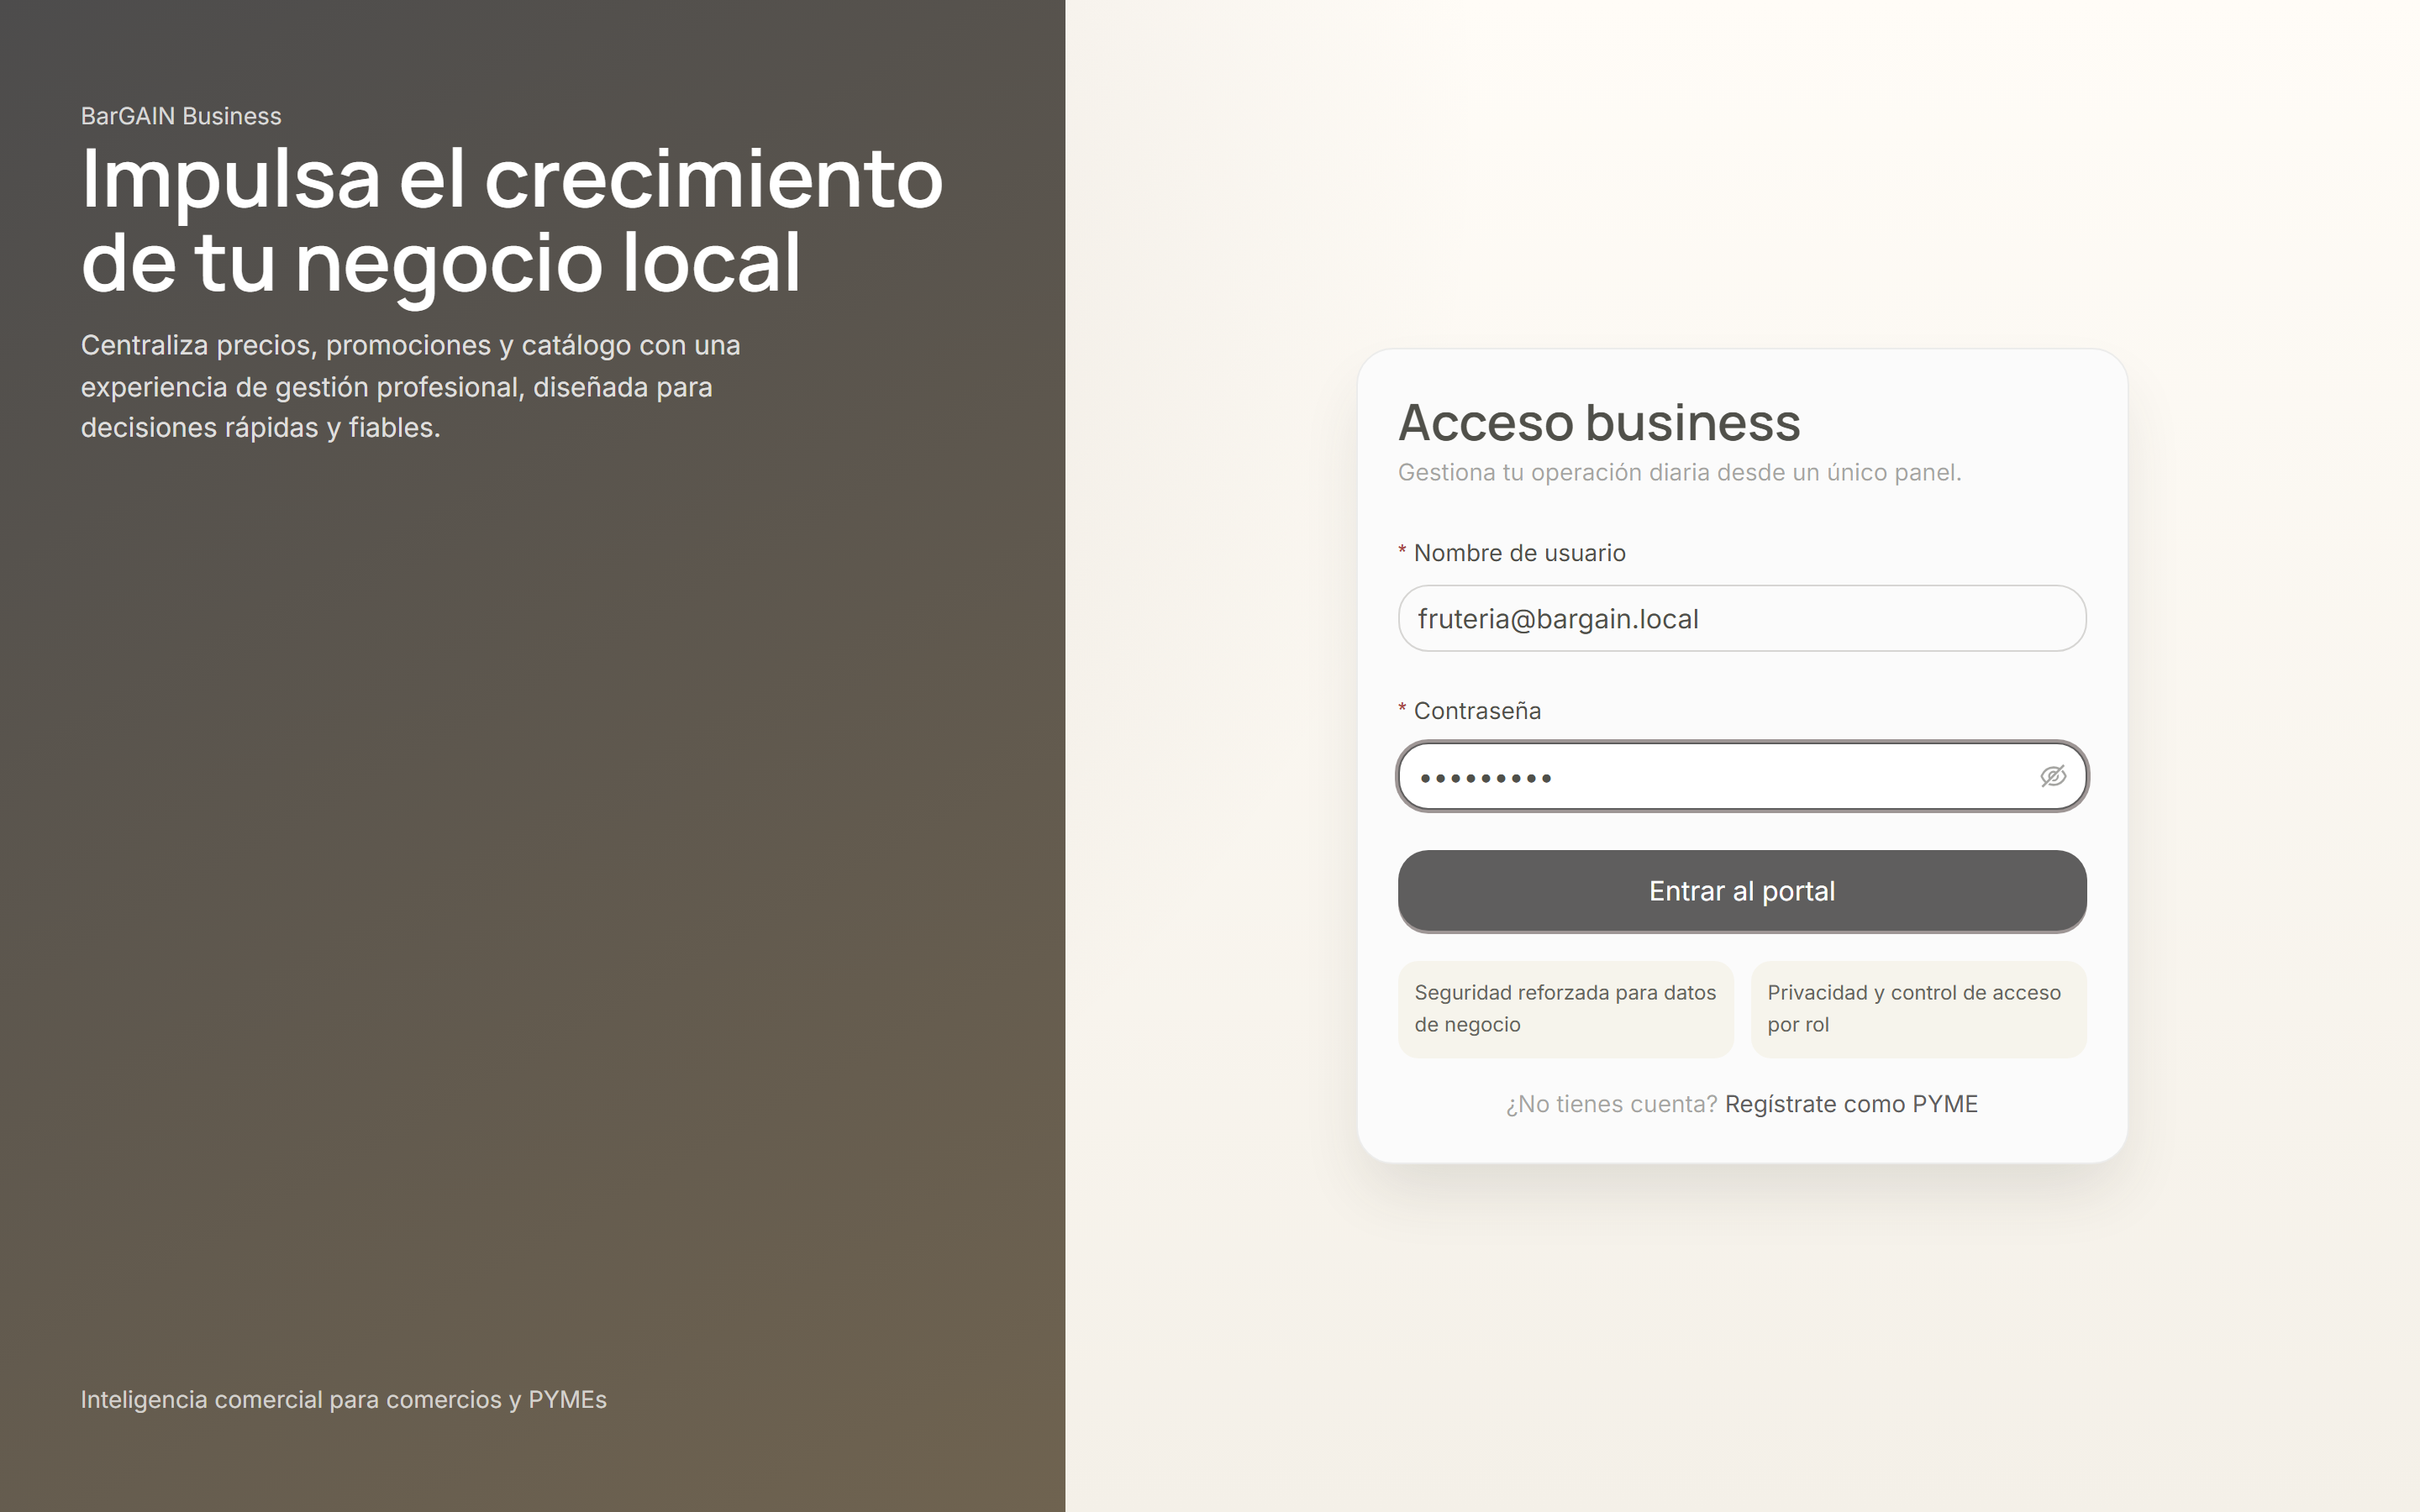
\includegraphics[width=0.46\textwidth]{diagramas/capturas/pyme-login.png}
\hfill
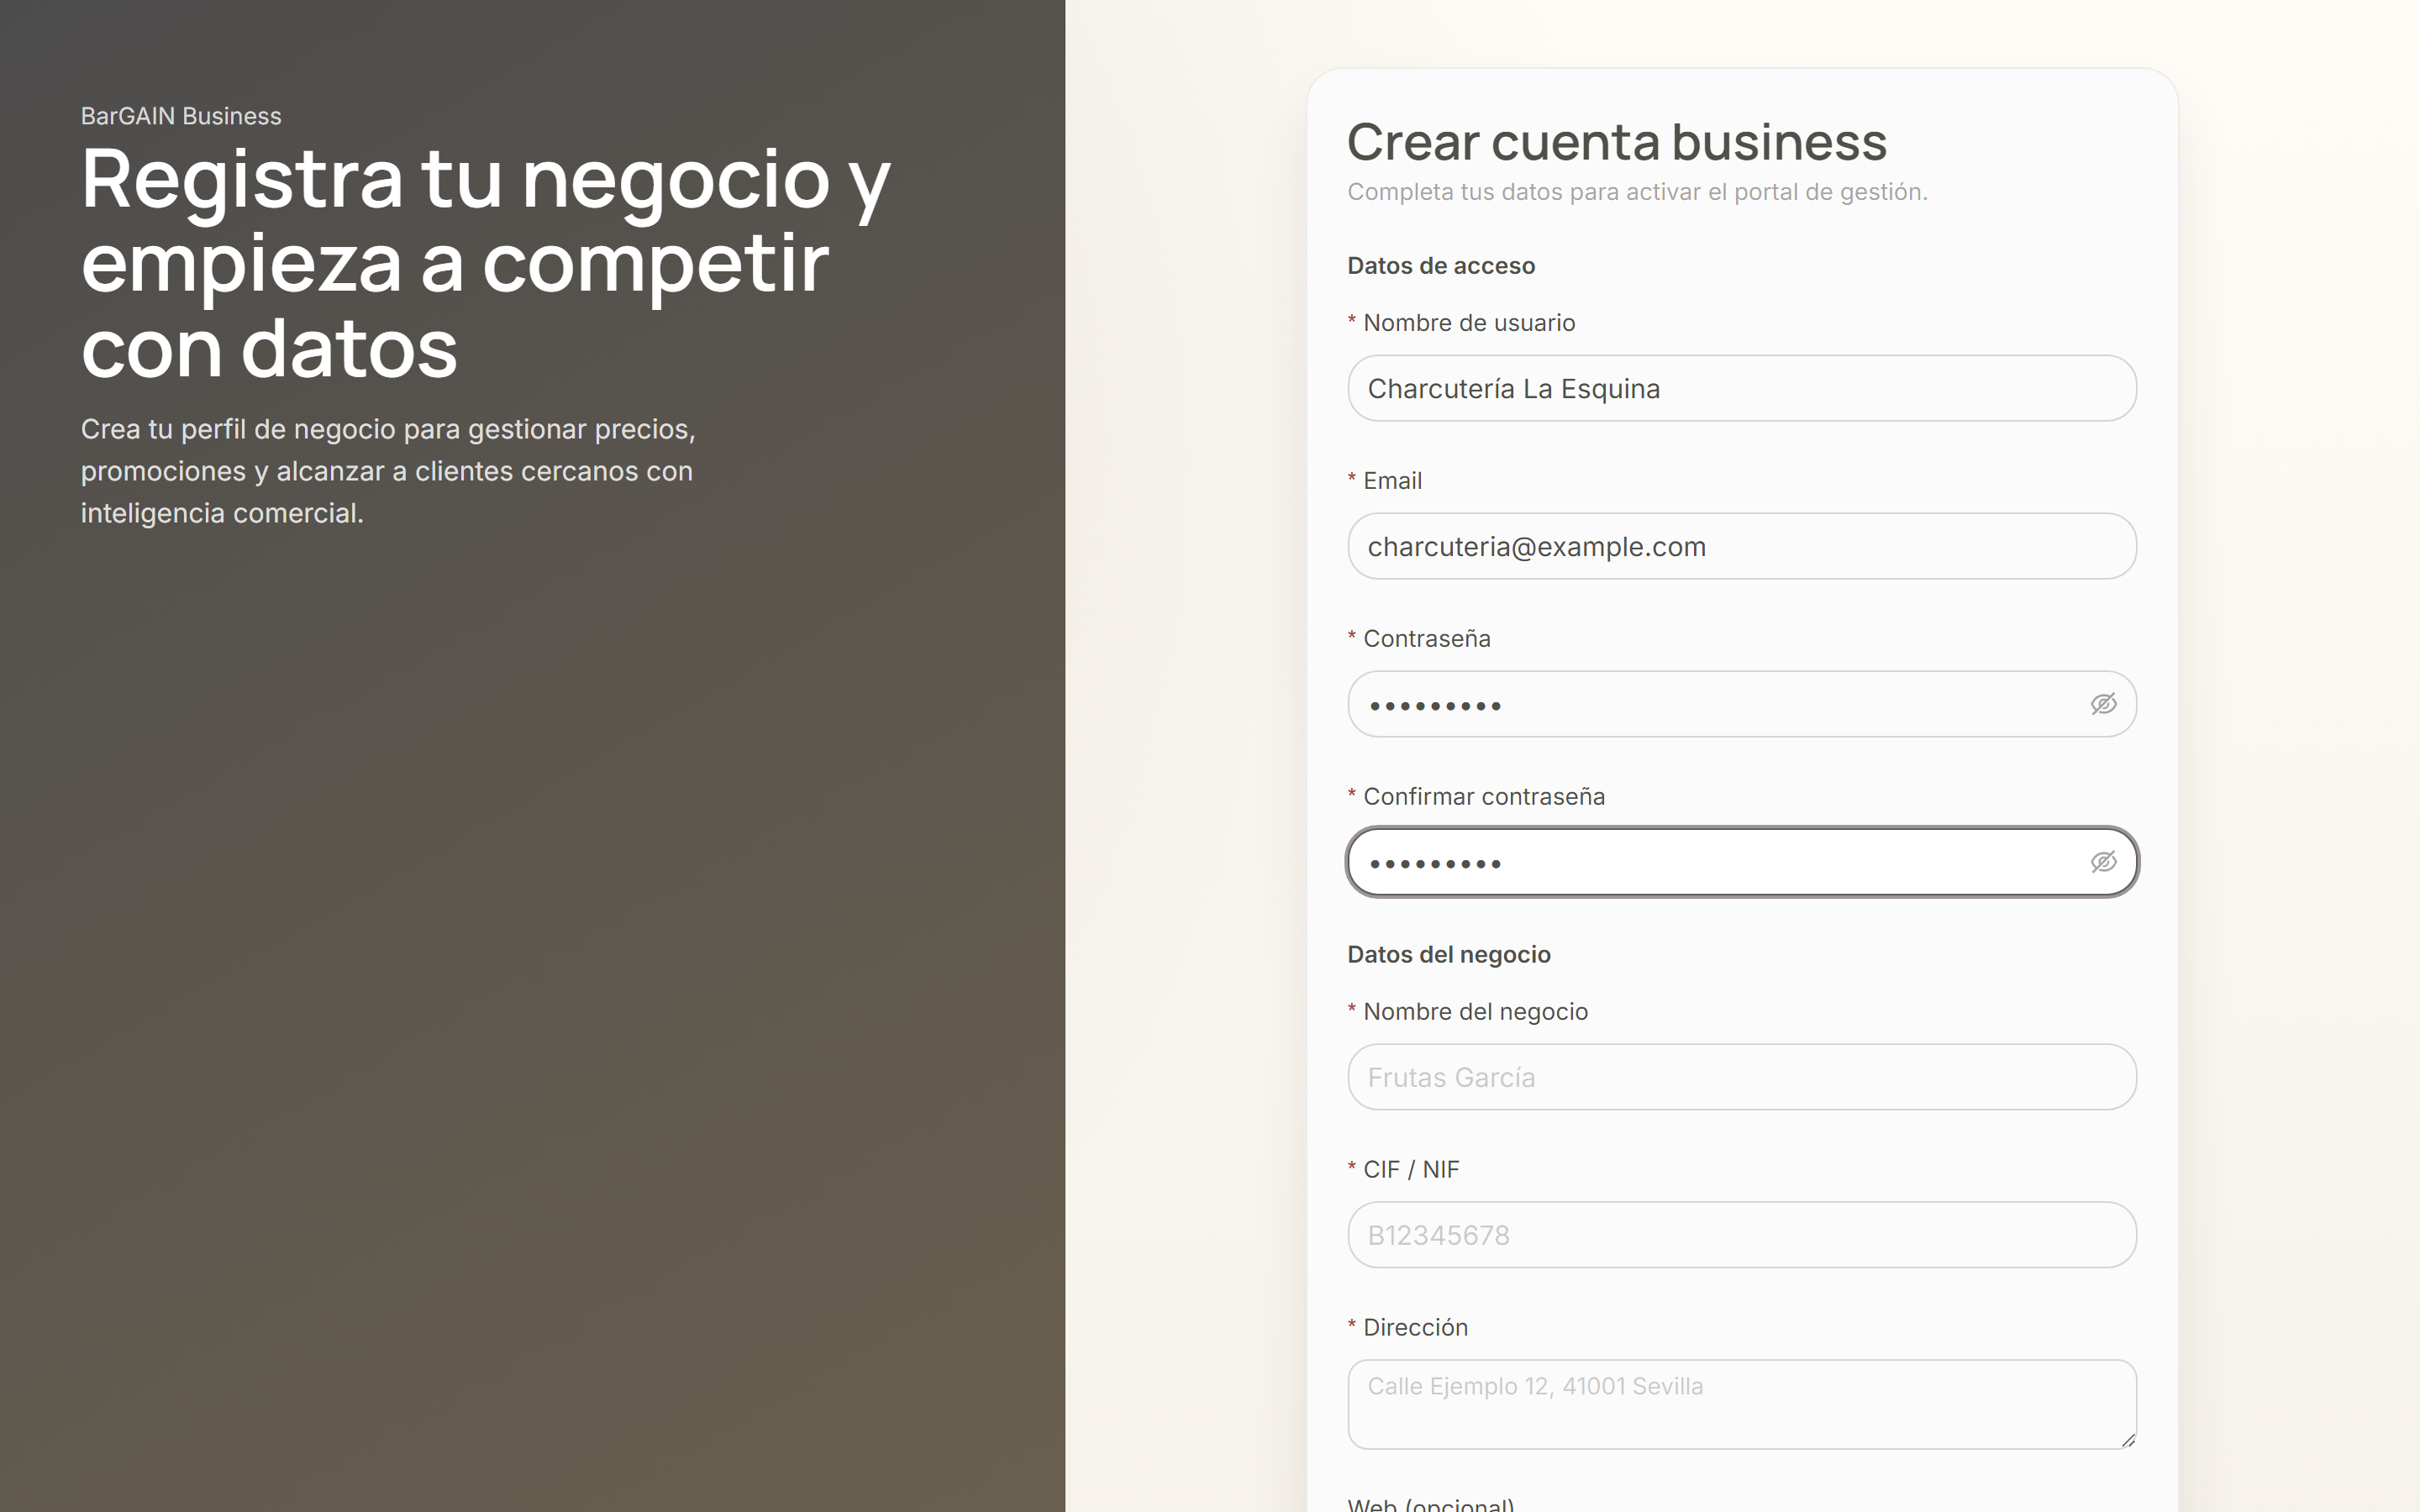
\includegraphics[width=0.46\textwidth]{diagramas/capturas/pyme-registro.png}
\caption{Portal PYME --- Inicio de sesi\'on (izquierda) y registro (derecha)}
\label{fig:cap-pyme-acceso}
\end{figure}

\begin{figure}[htbp]
\centering
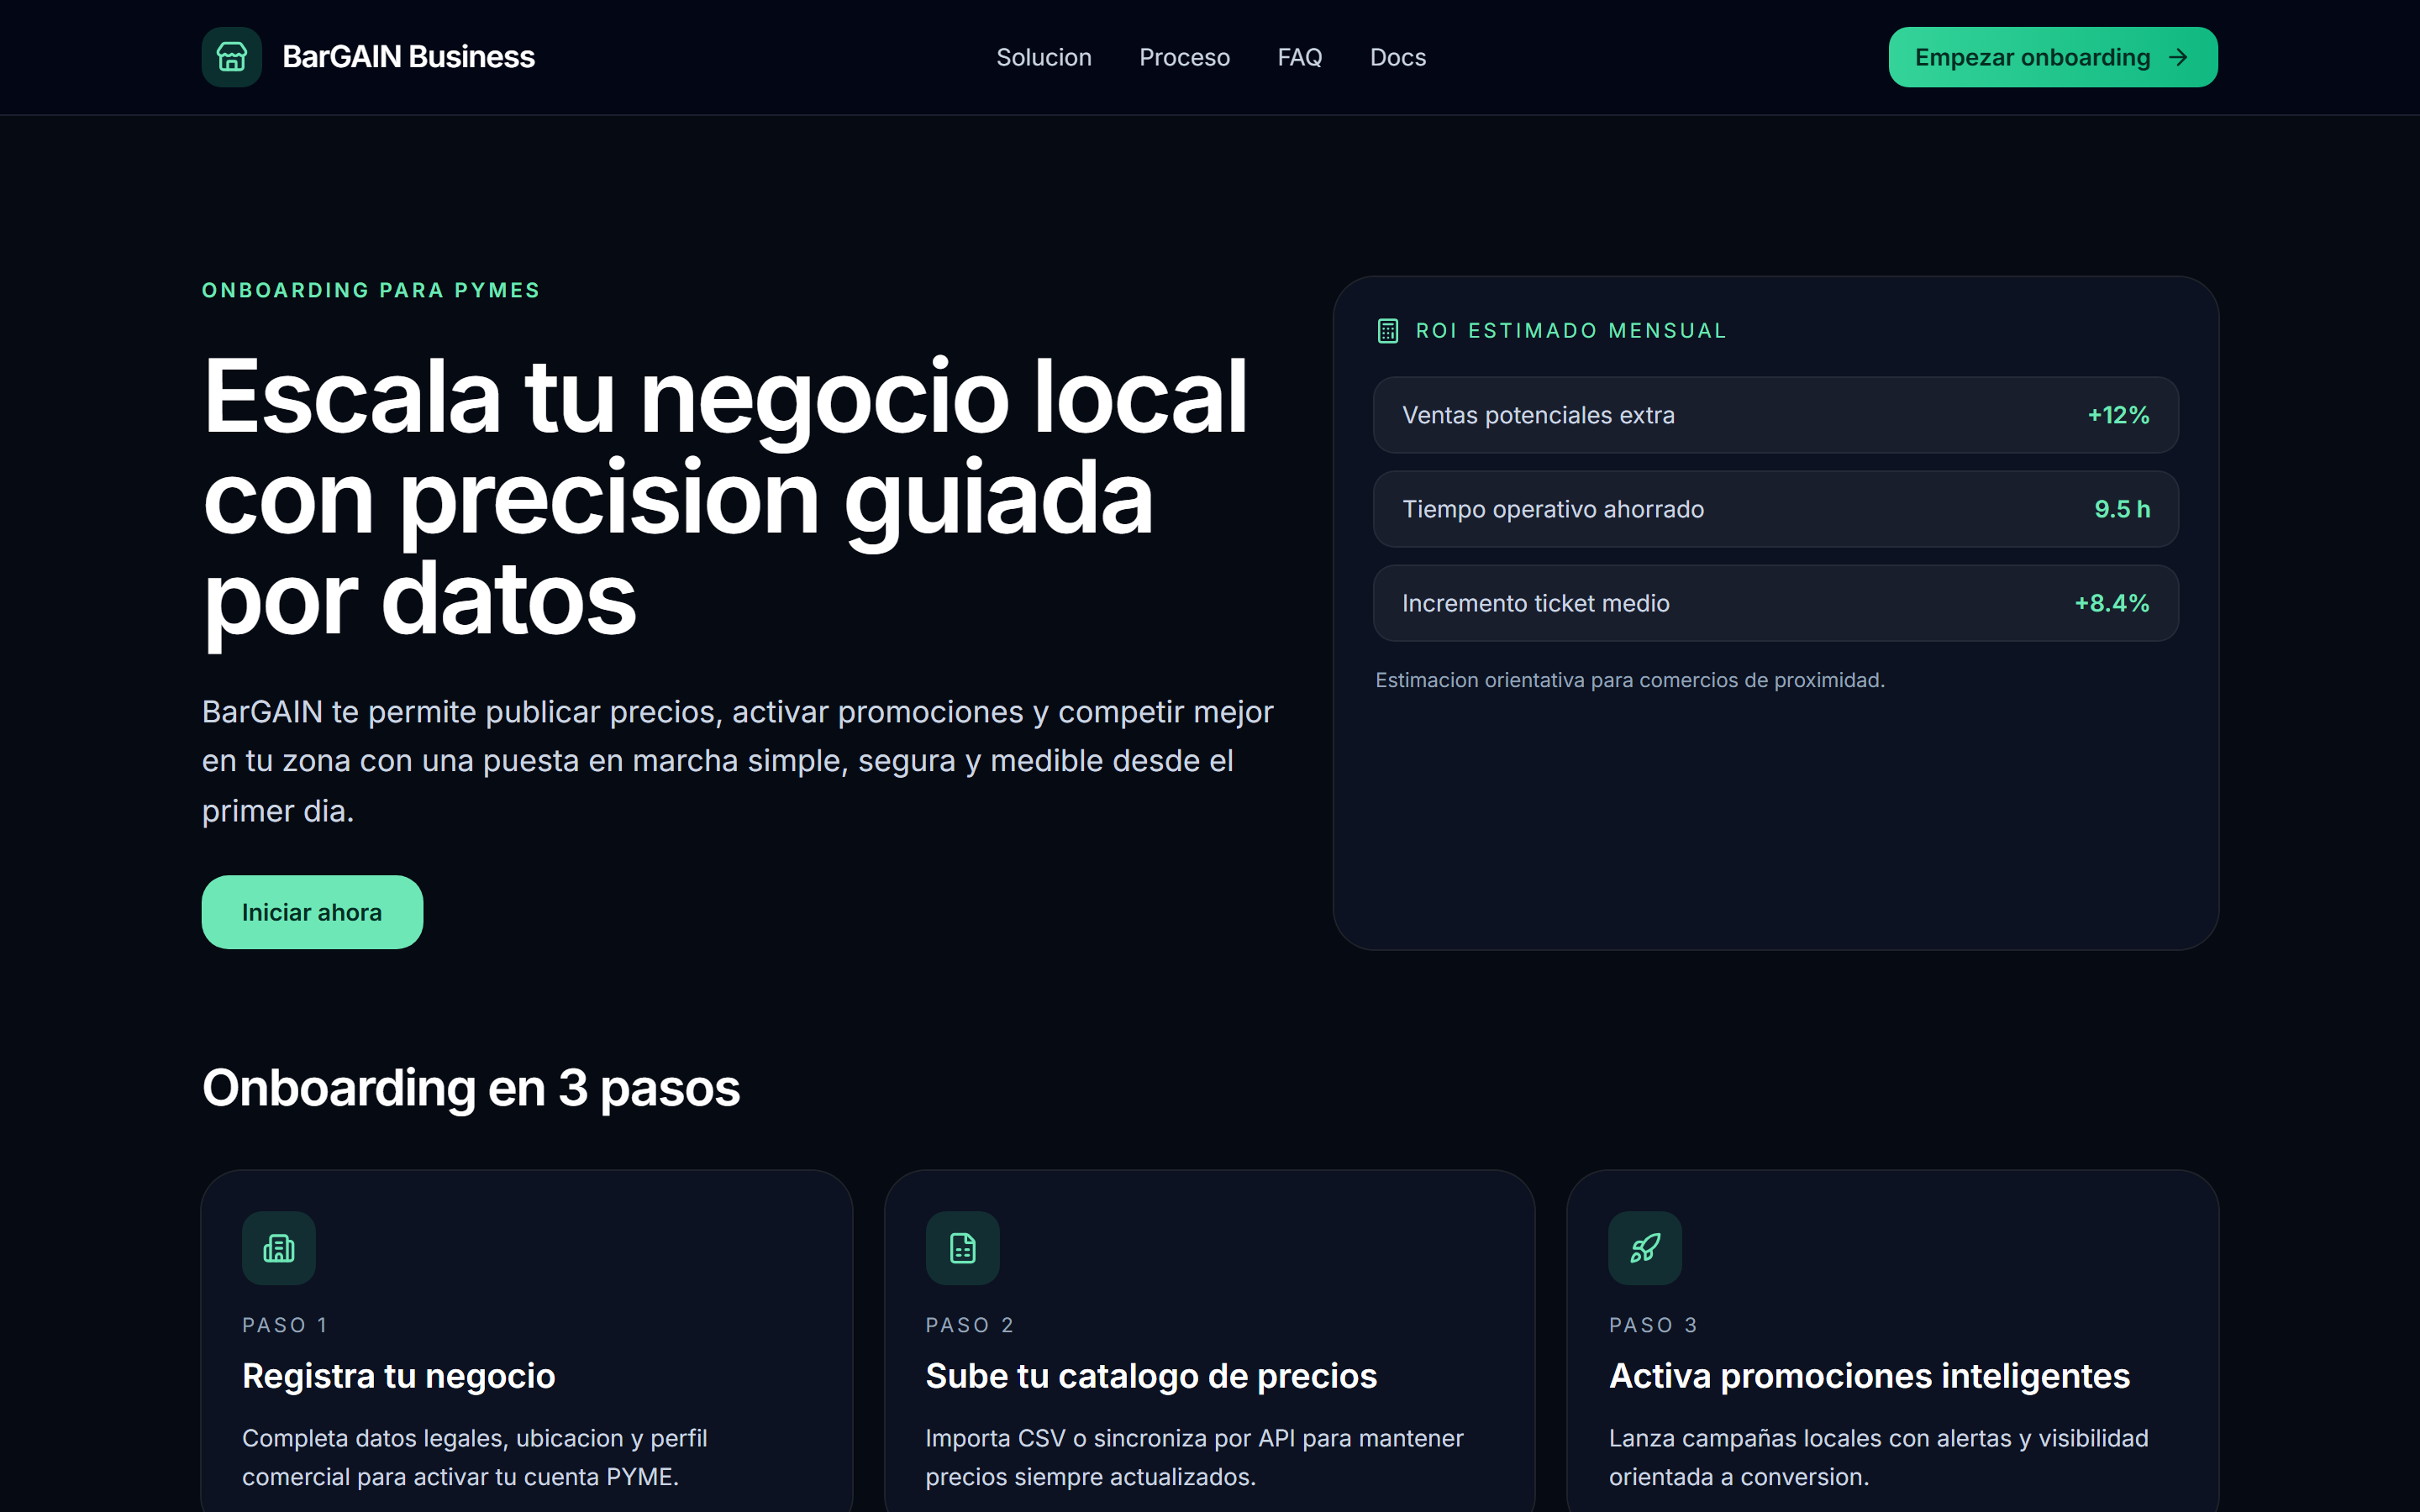
\includegraphics[width=0.85\textwidth]{diagramas/capturas/pyme-onboarding.png}
\caption{Portal PYME --- Onboarding del negocio (alta de datos y CIF)}
\label{fig:cap-pyme-onboarding}
\end{figure}

\begin{figure}[htbp]
\centering
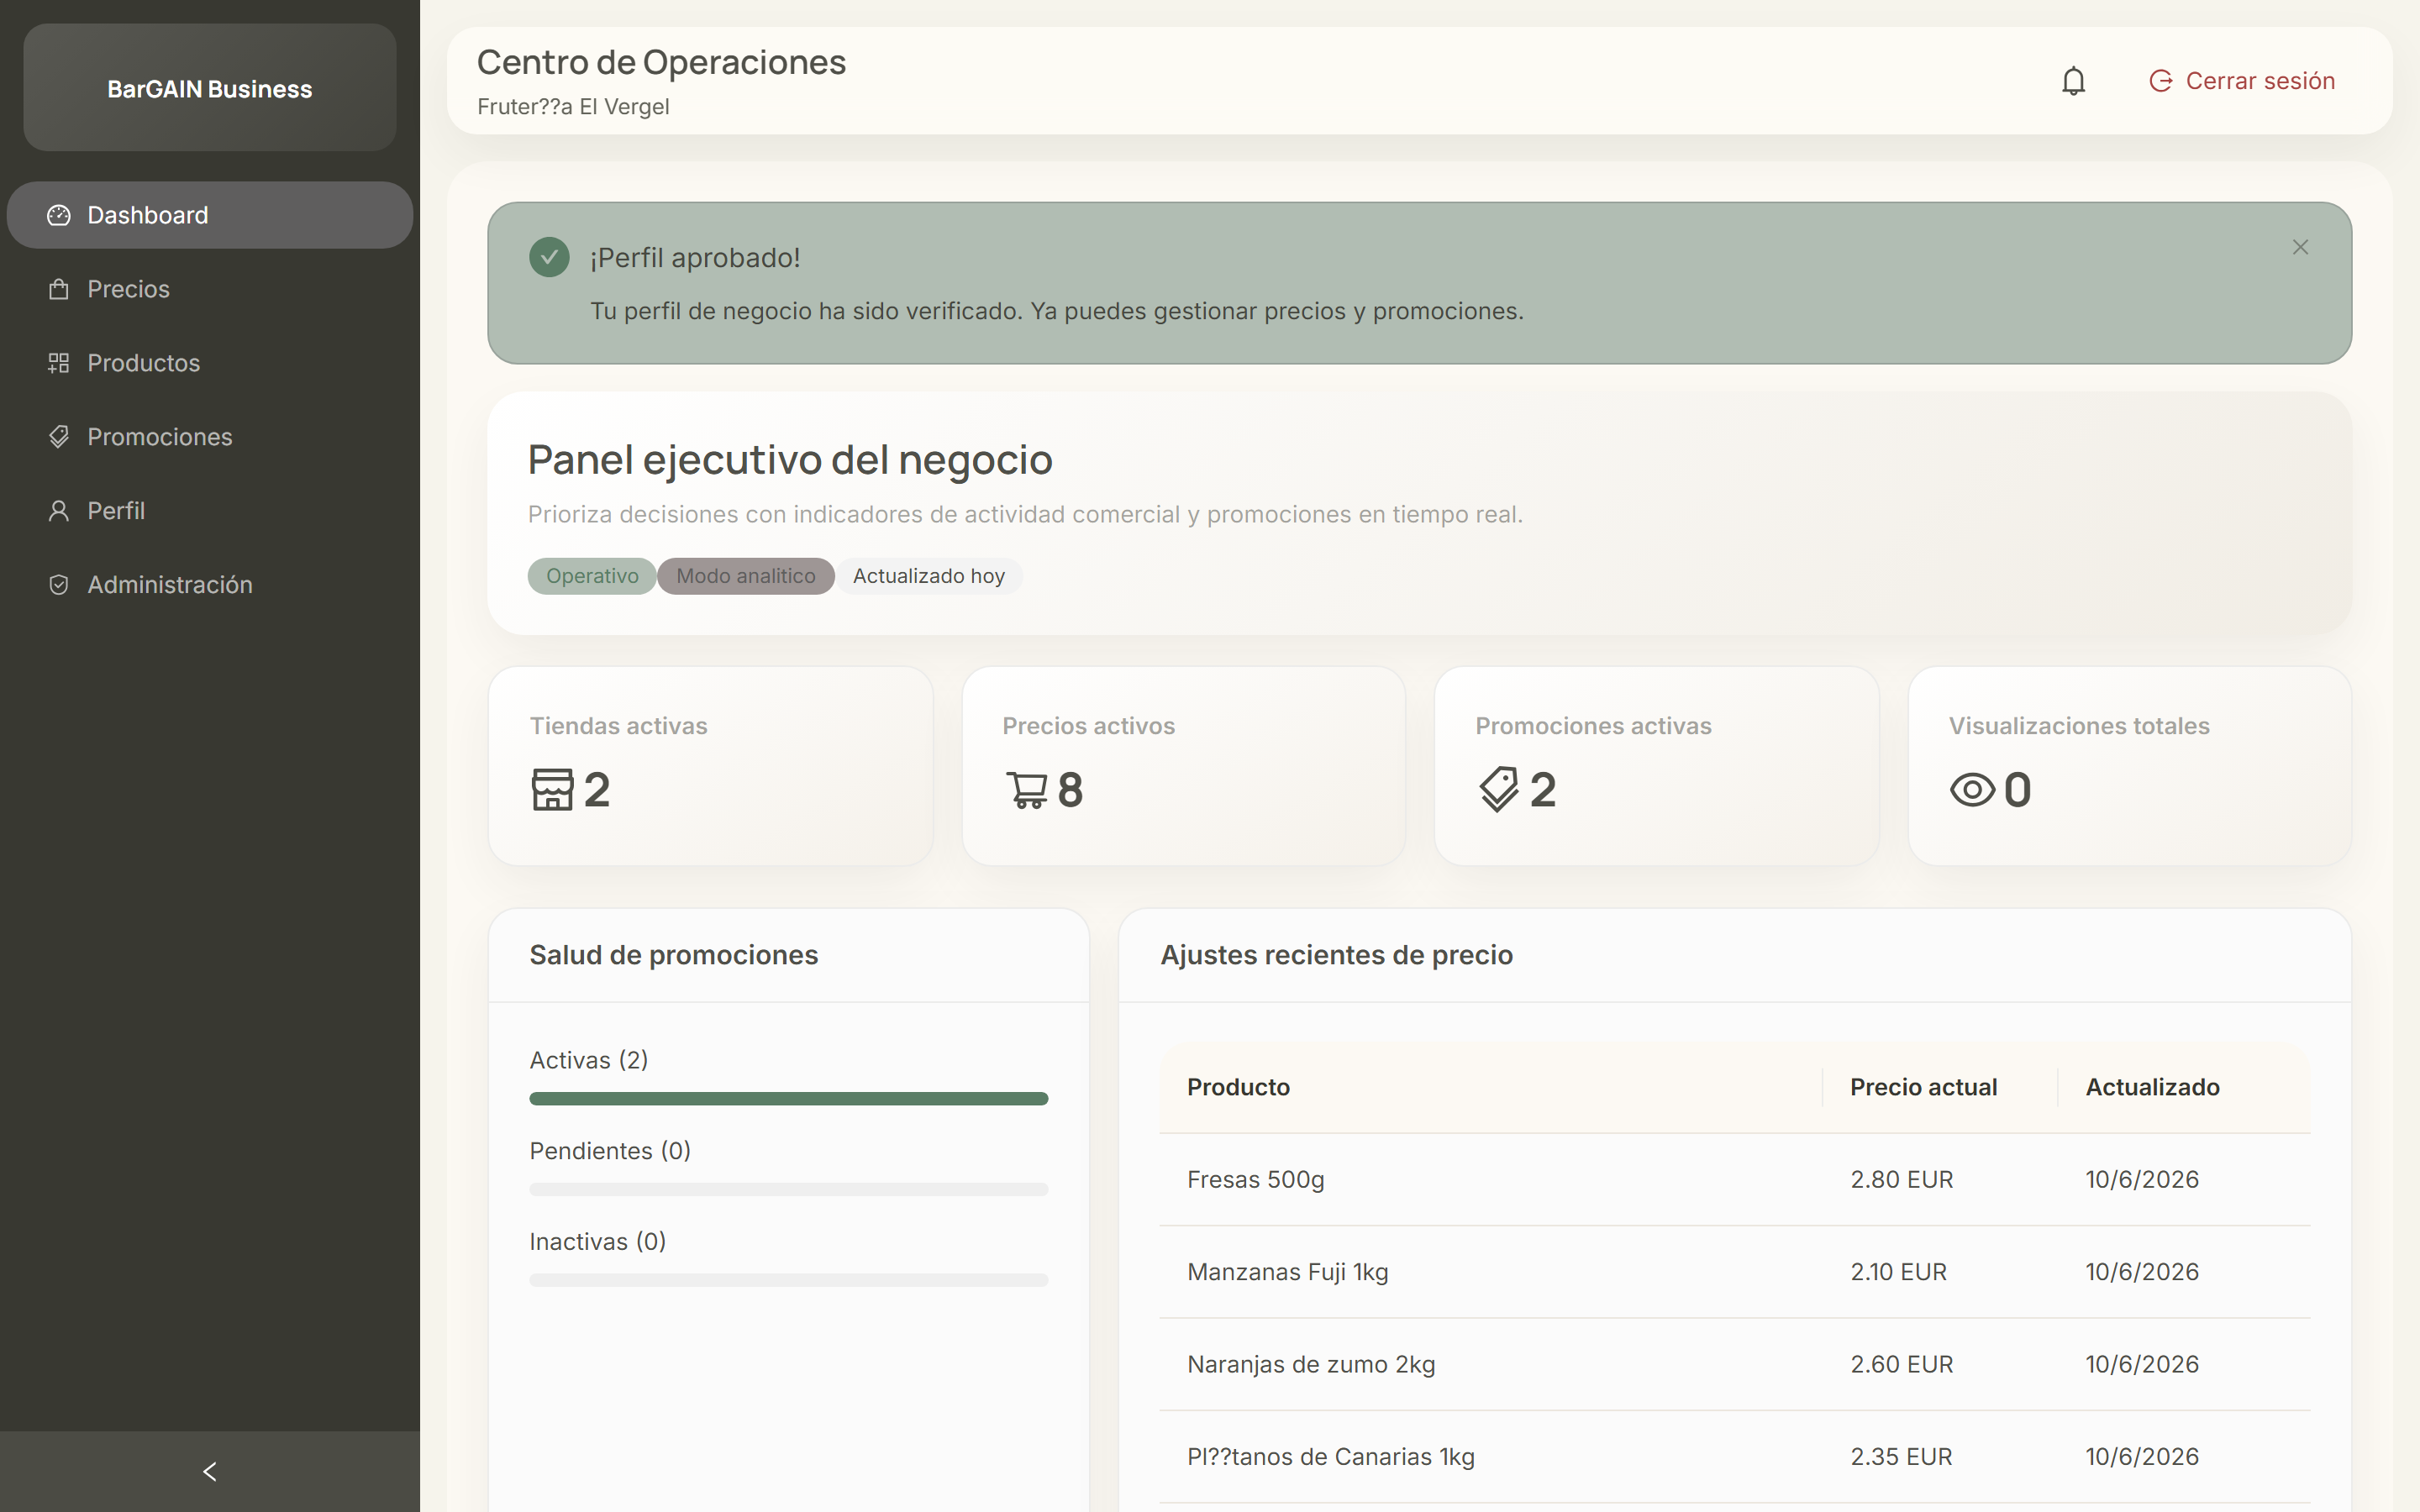
\includegraphics[width=0.85\textwidth]{diagramas/capturas/pyme-dashboard.png}
\caption{Portal PYME --- Panel de control (\emph{dashboard}) con estad\'isticas}
\label{fig:cap-pyme-dashboard}
\end{figure}

\clearpage

\begin{figure}[htbp]
\centering
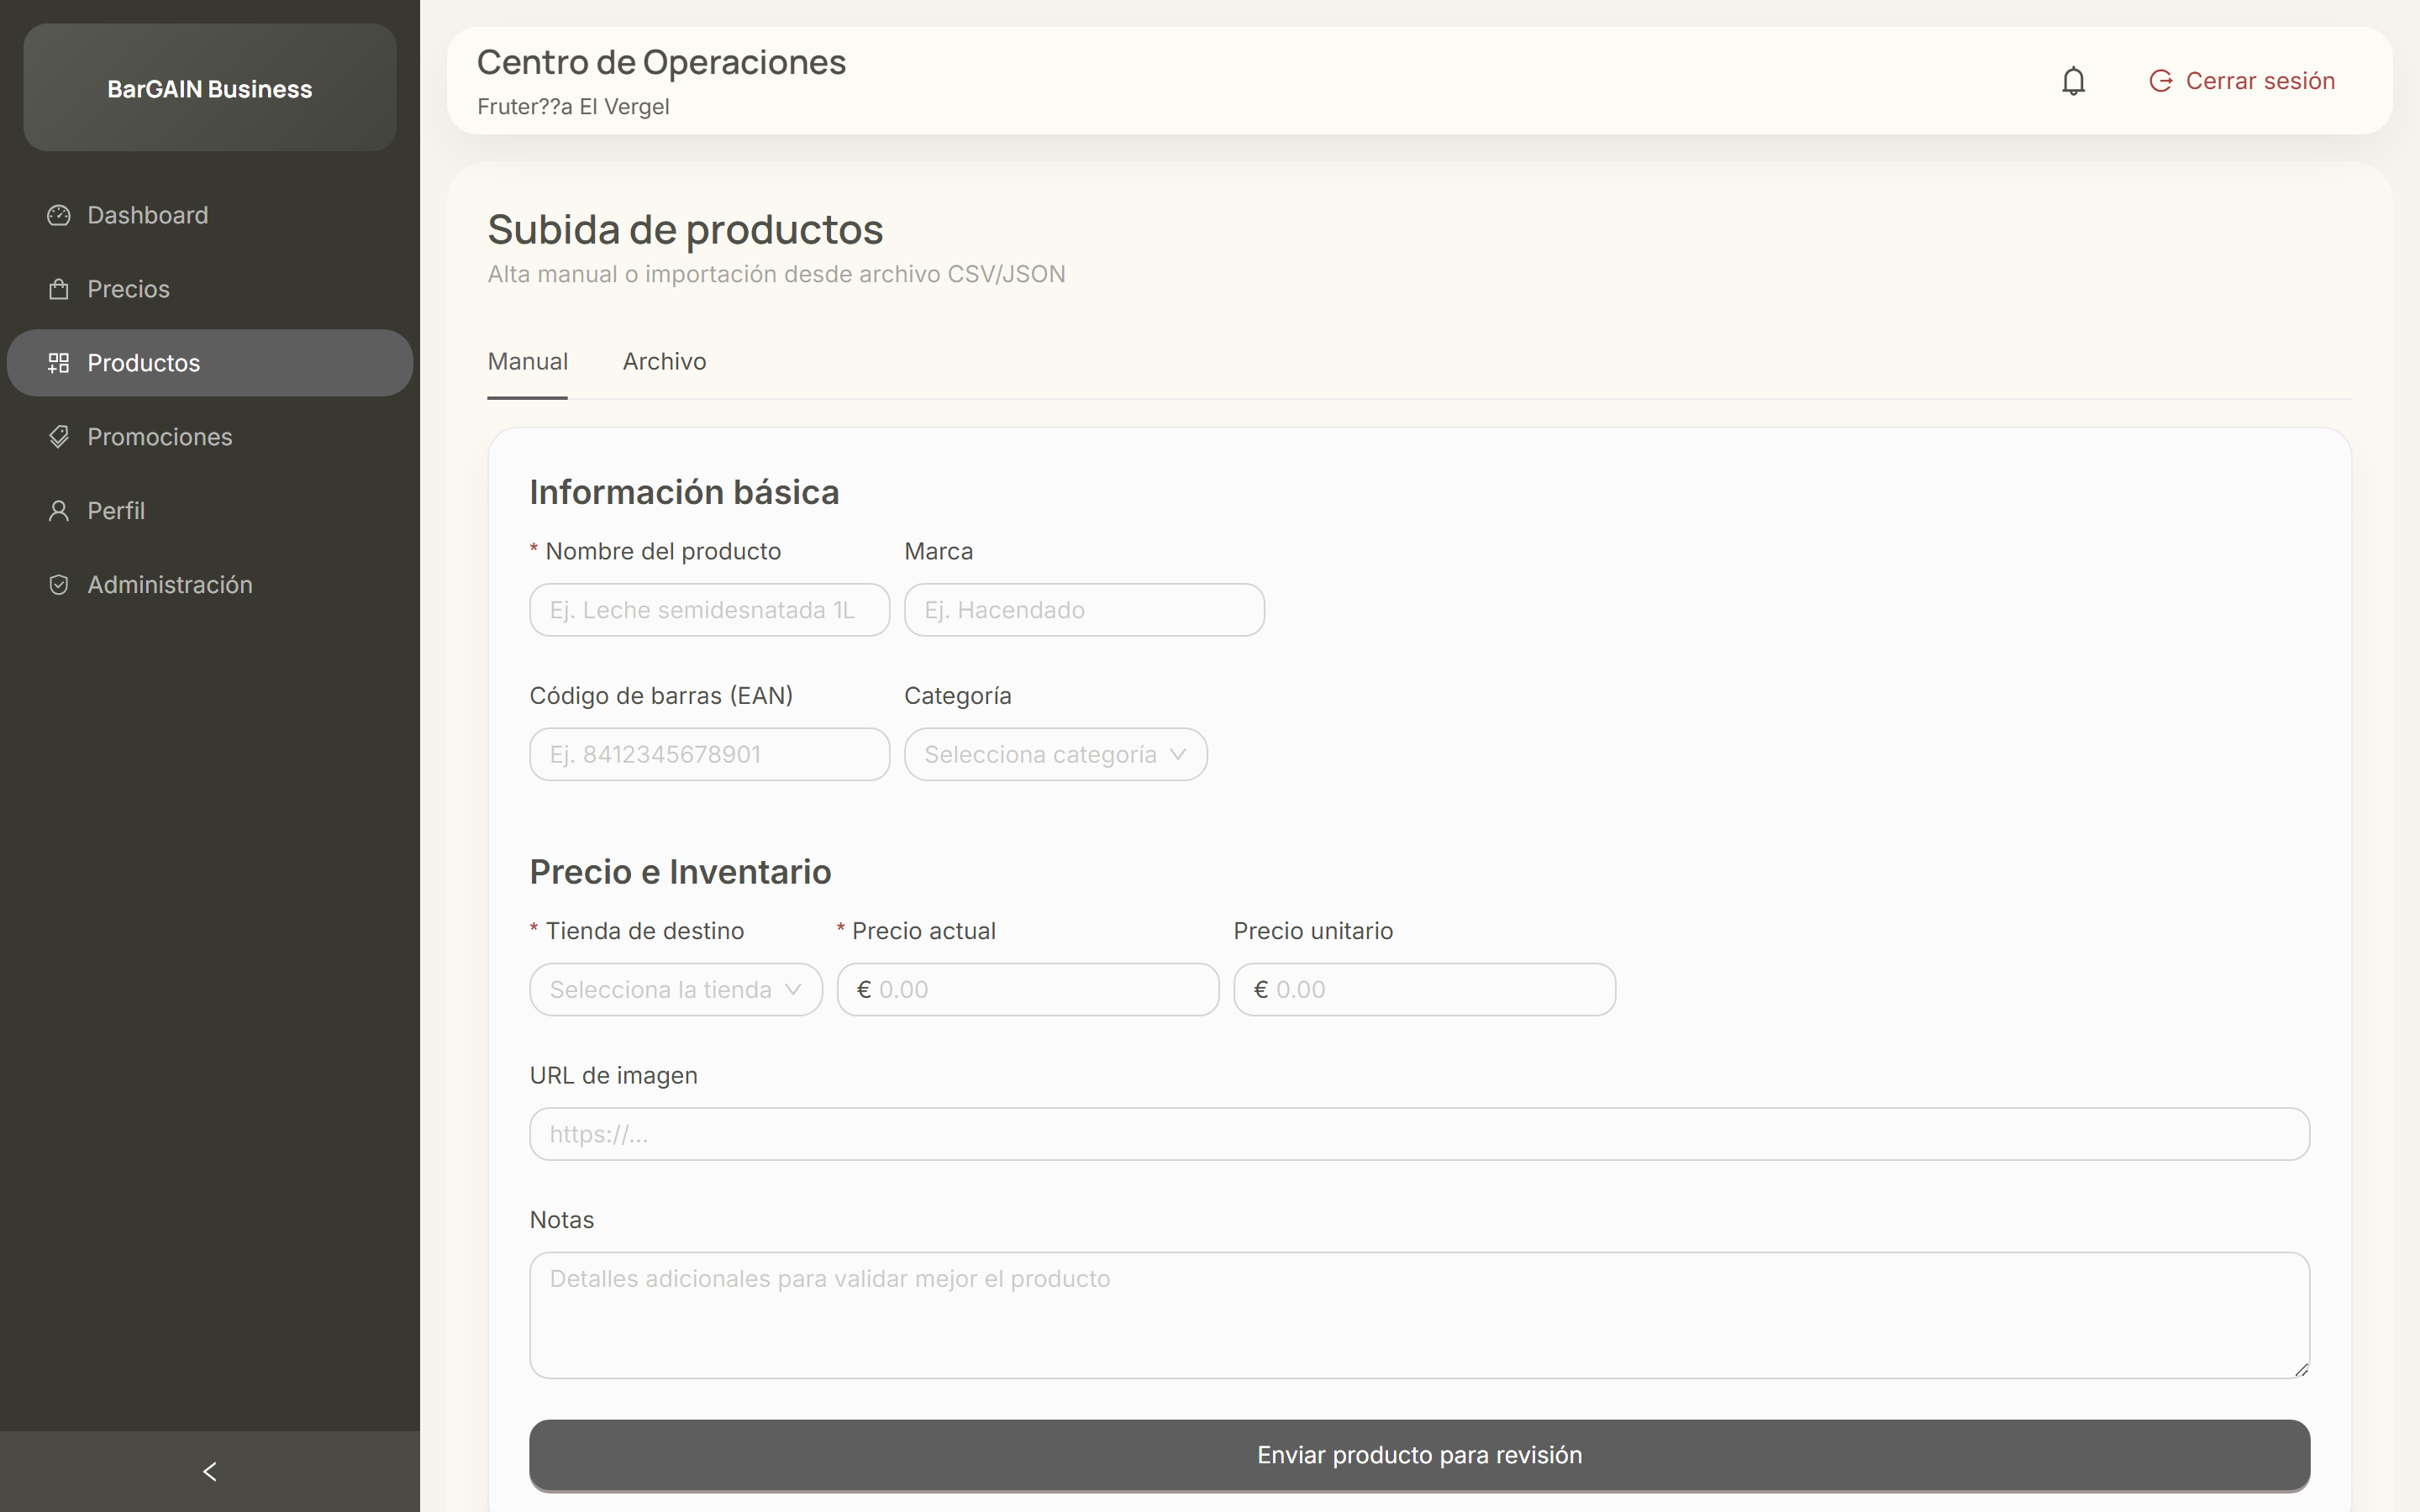
\includegraphics[width=0.46\textwidth]{diagramas/capturas/pyme-productos.png}
\hfill
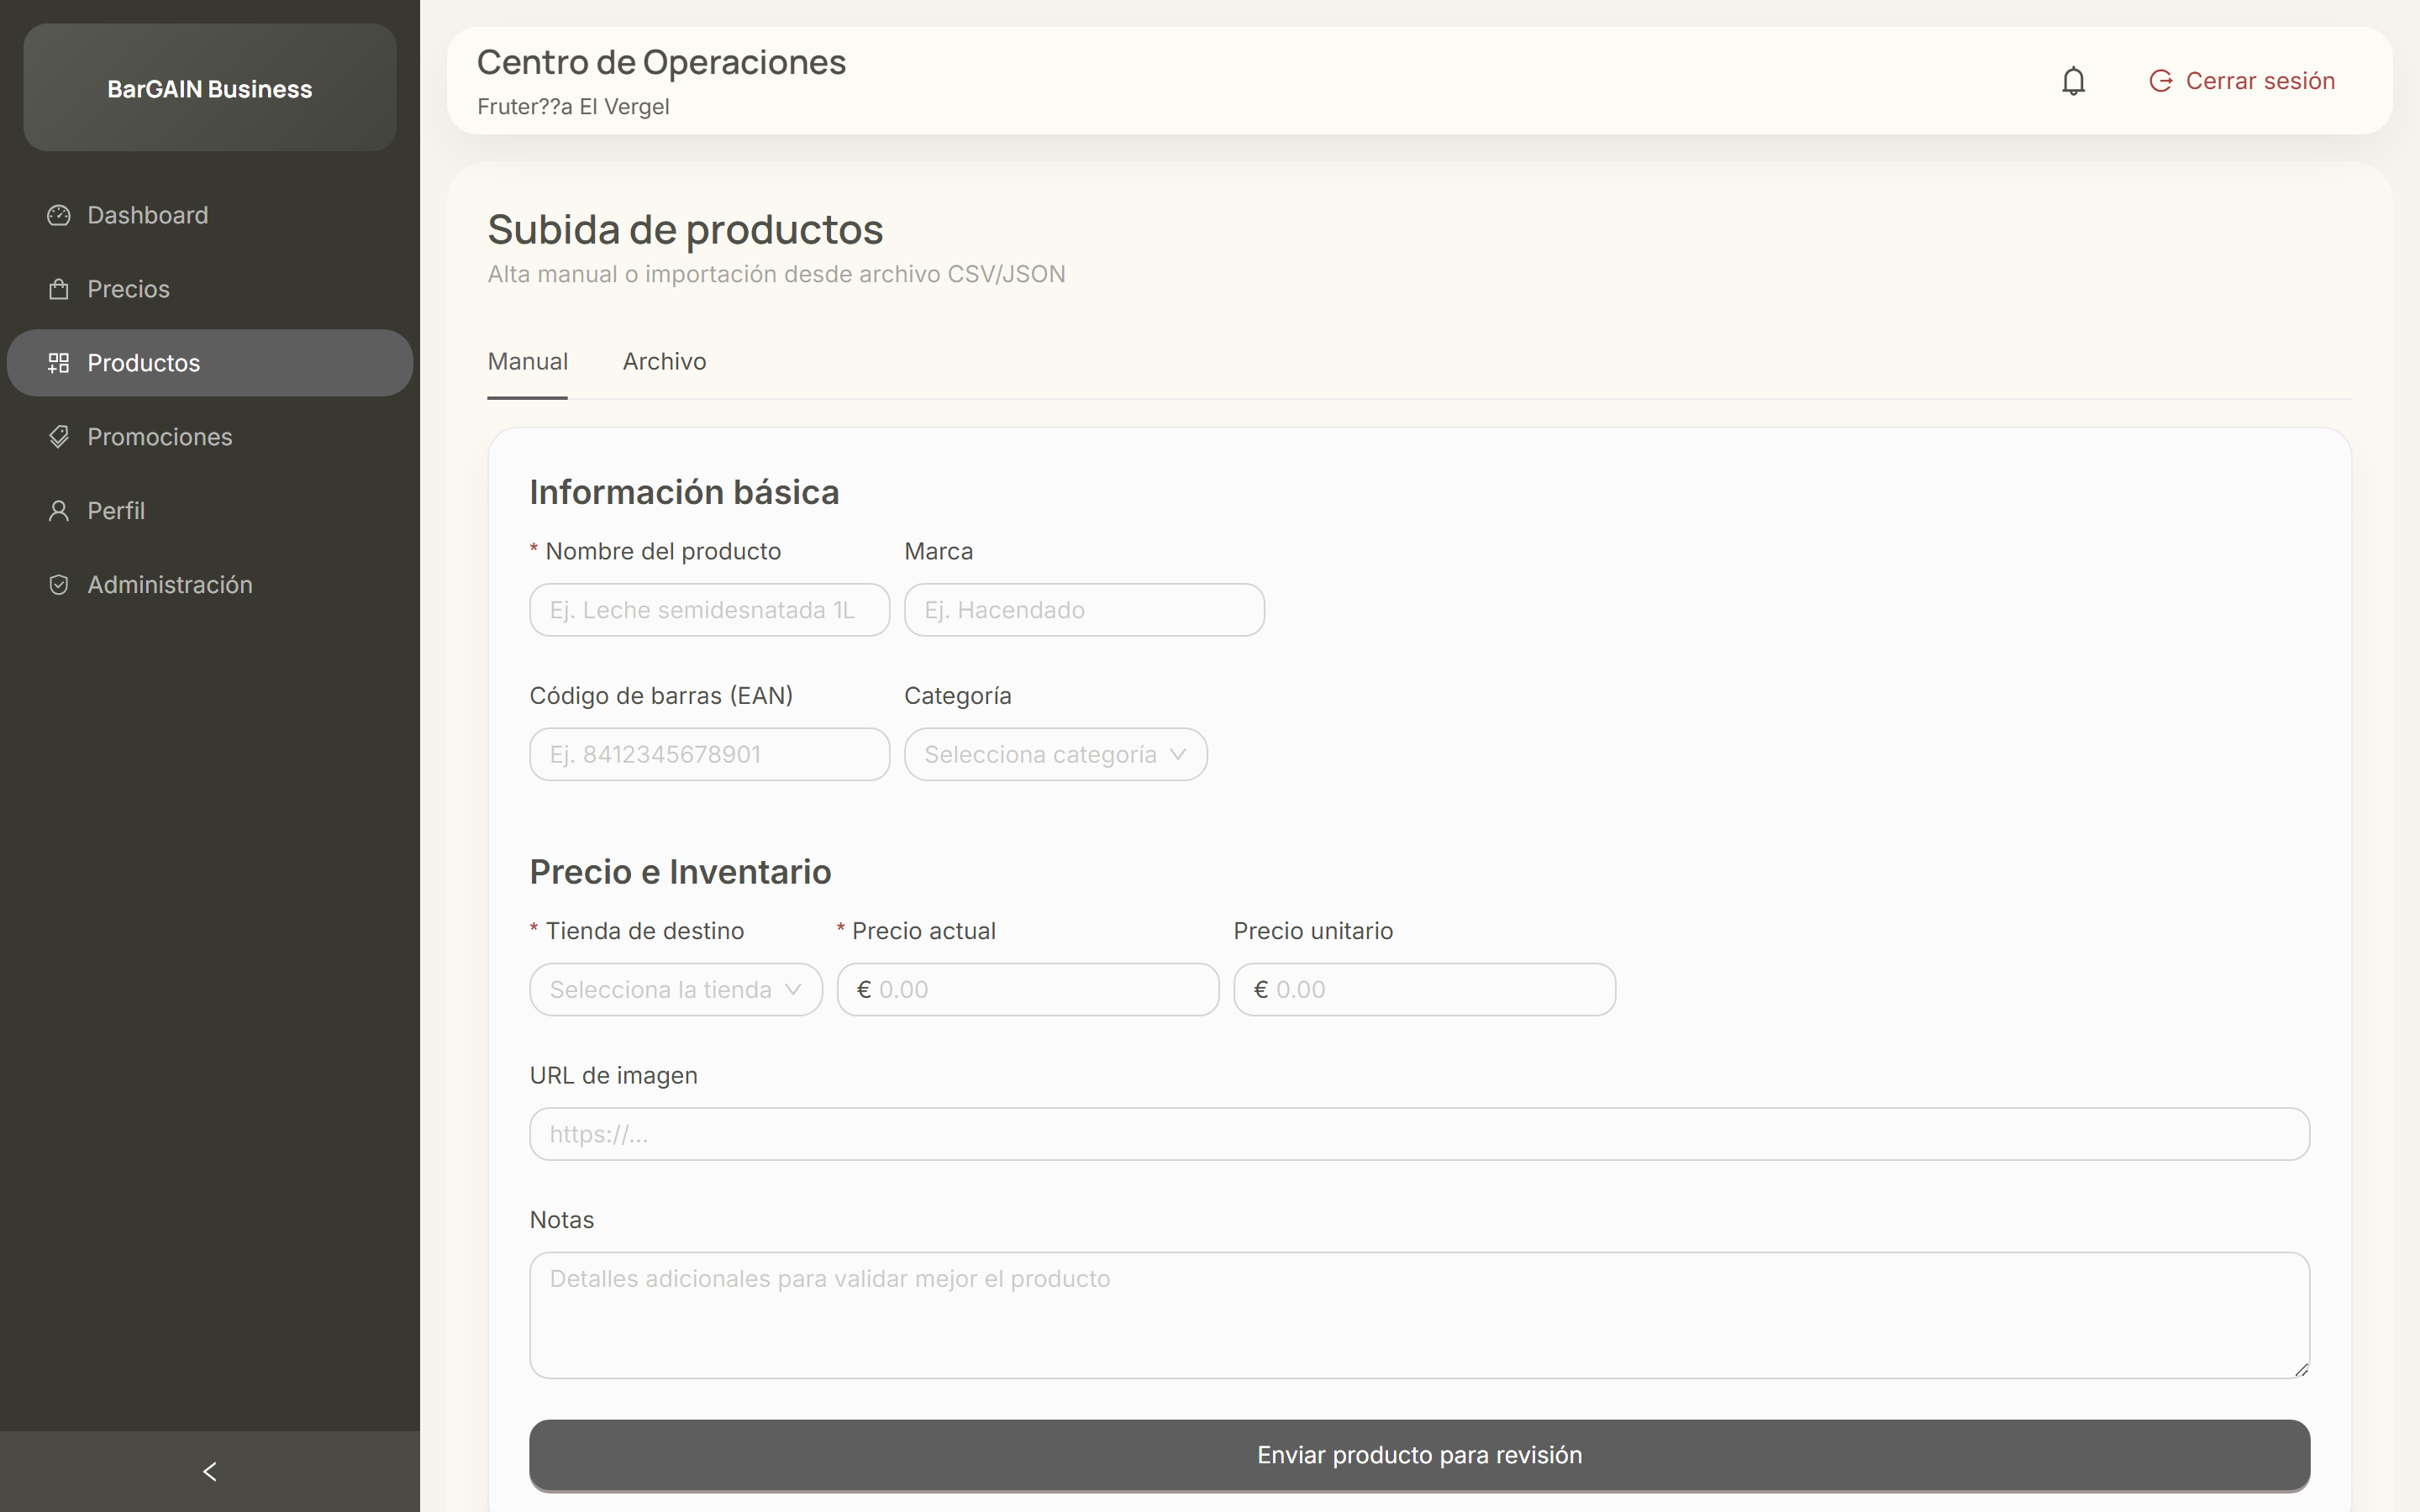
\includegraphics[width=0.46\textwidth]{diagramas/capturas/pyme-carga-masiva.png}
\caption{Portal PYME --- Gesti\'on de productos (izquierda) y carga masiva por CSV (derecha)}
\label{fig:cap-pyme-productos}
\end{figure}

\begin{figure}[htbp]
\centering
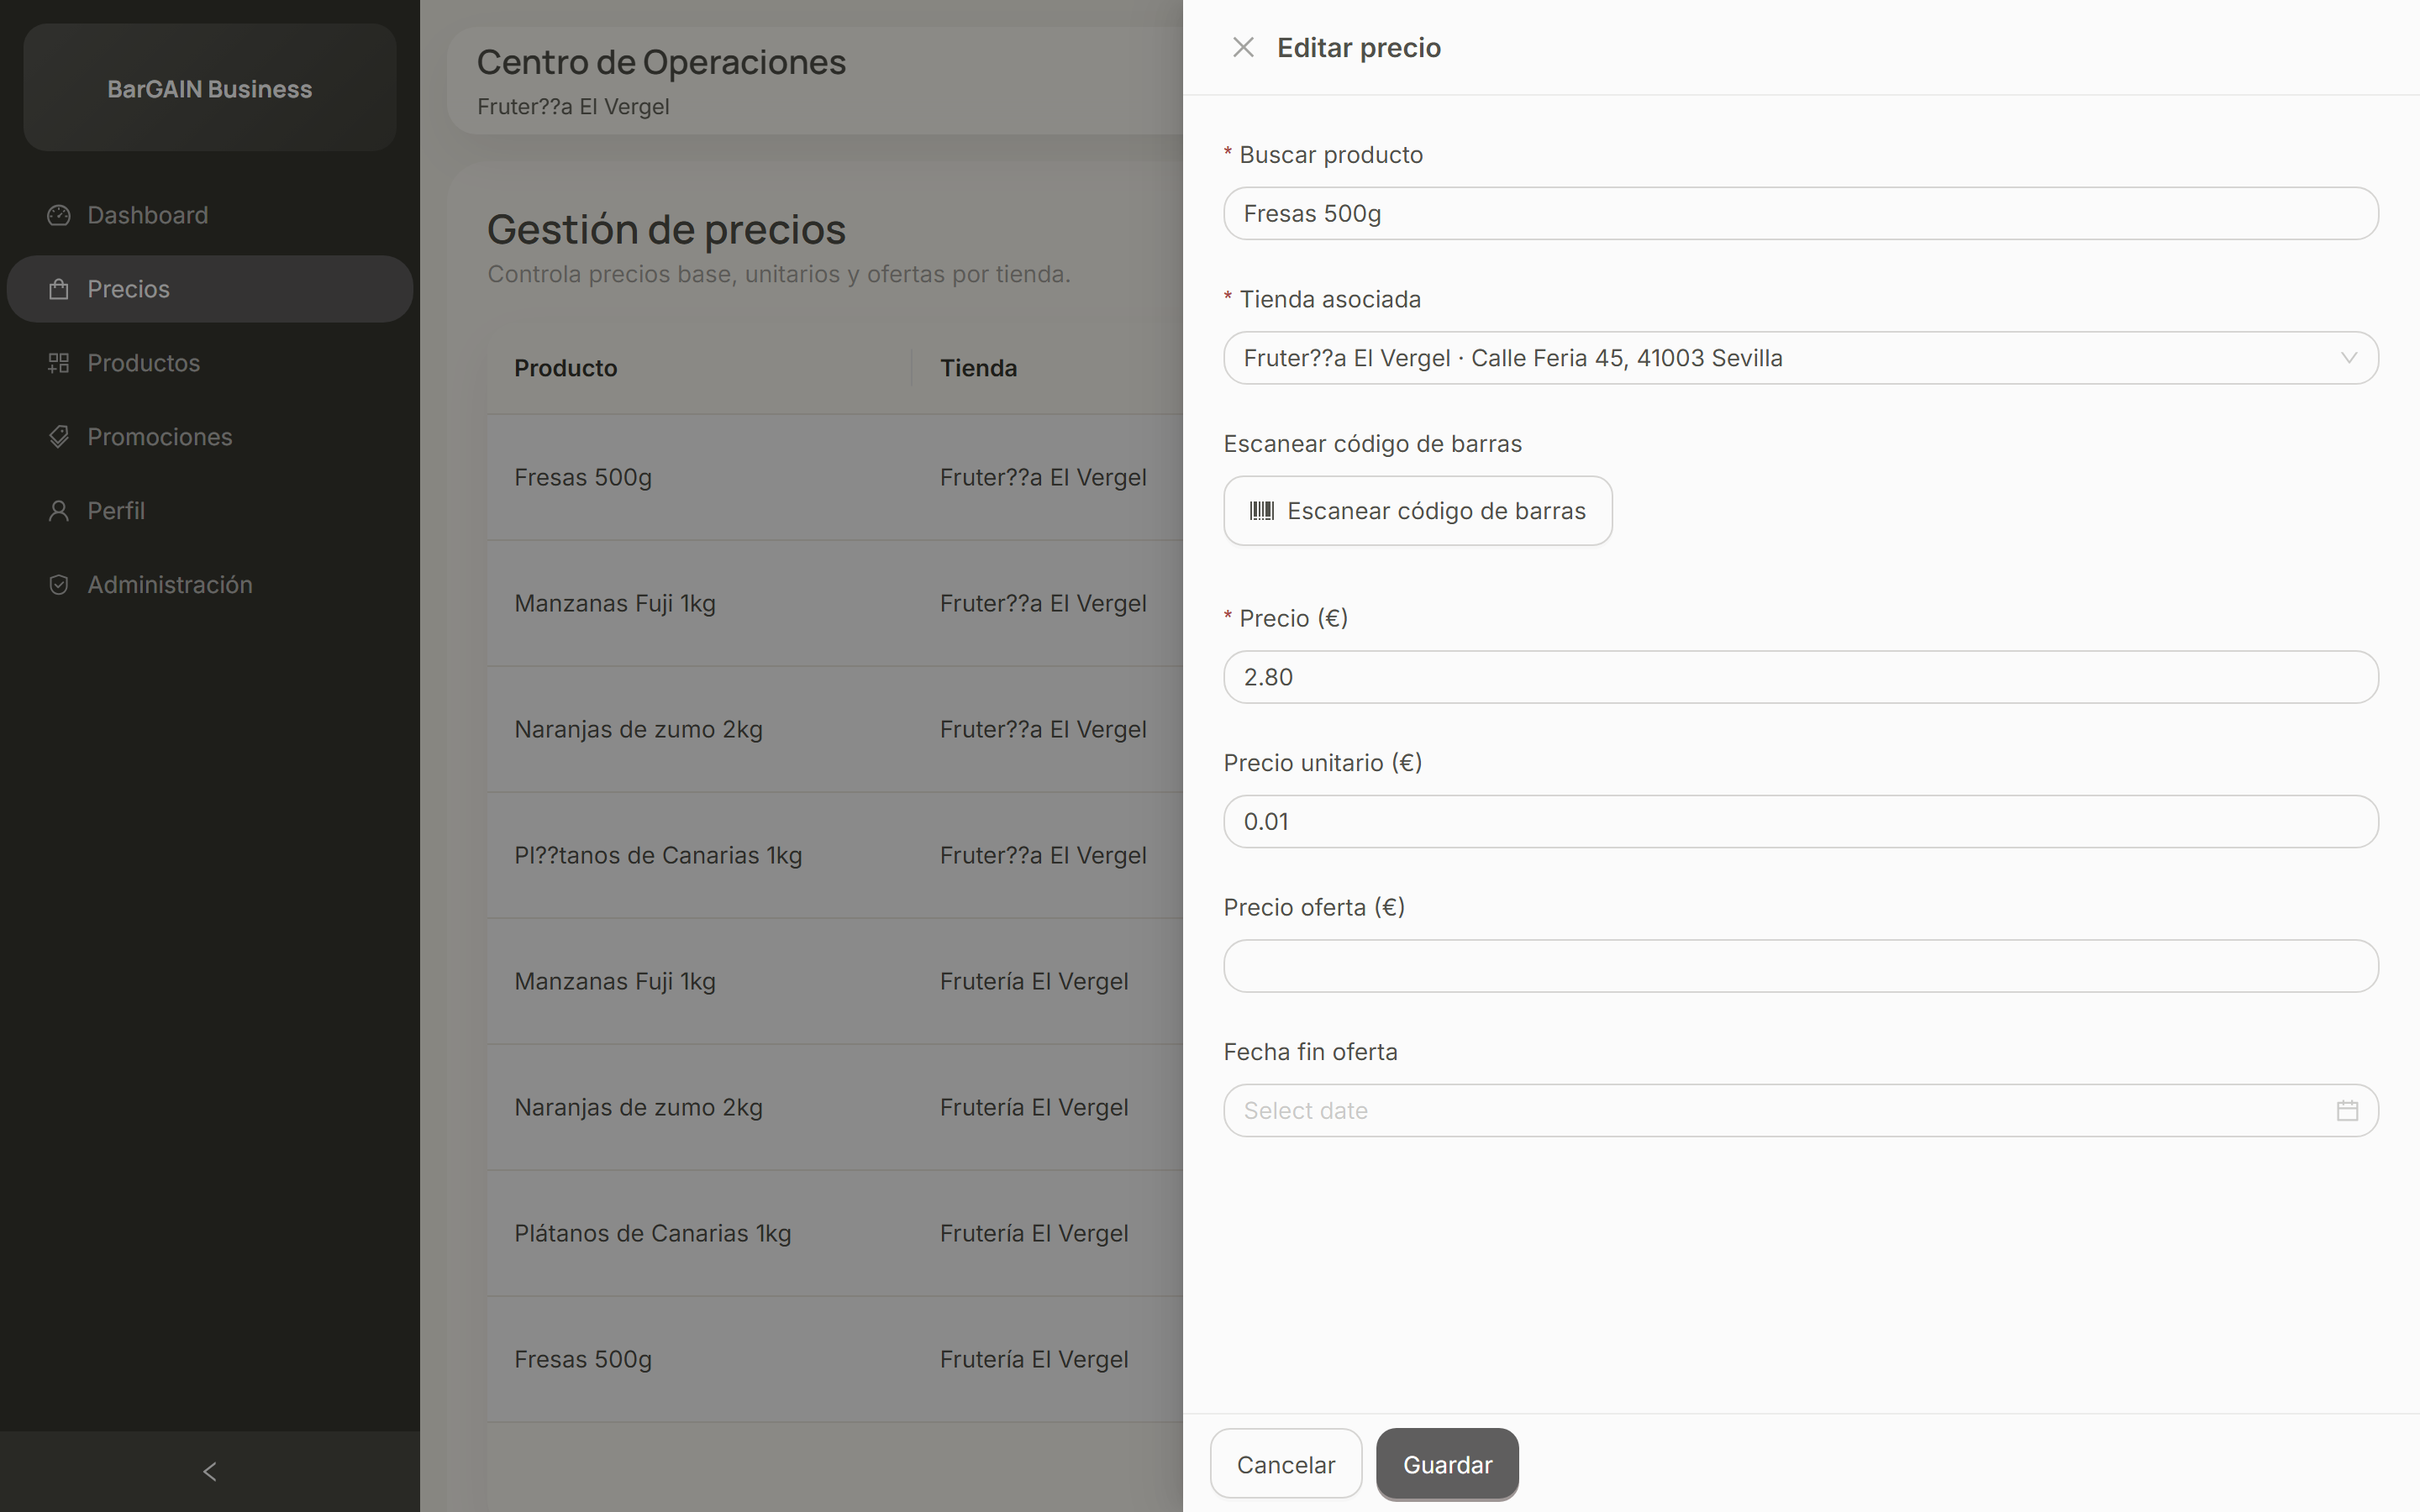
\includegraphics[width=0.85\textwidth]{diagramas/capturas/pyme-precios.png}
\caption{Portal PYME --- Gesti\'on de precios (tabla editable)}
\label{fig:cap-pyme-precios}
\end{figure}

\begin{figure}[htbp]
\centering
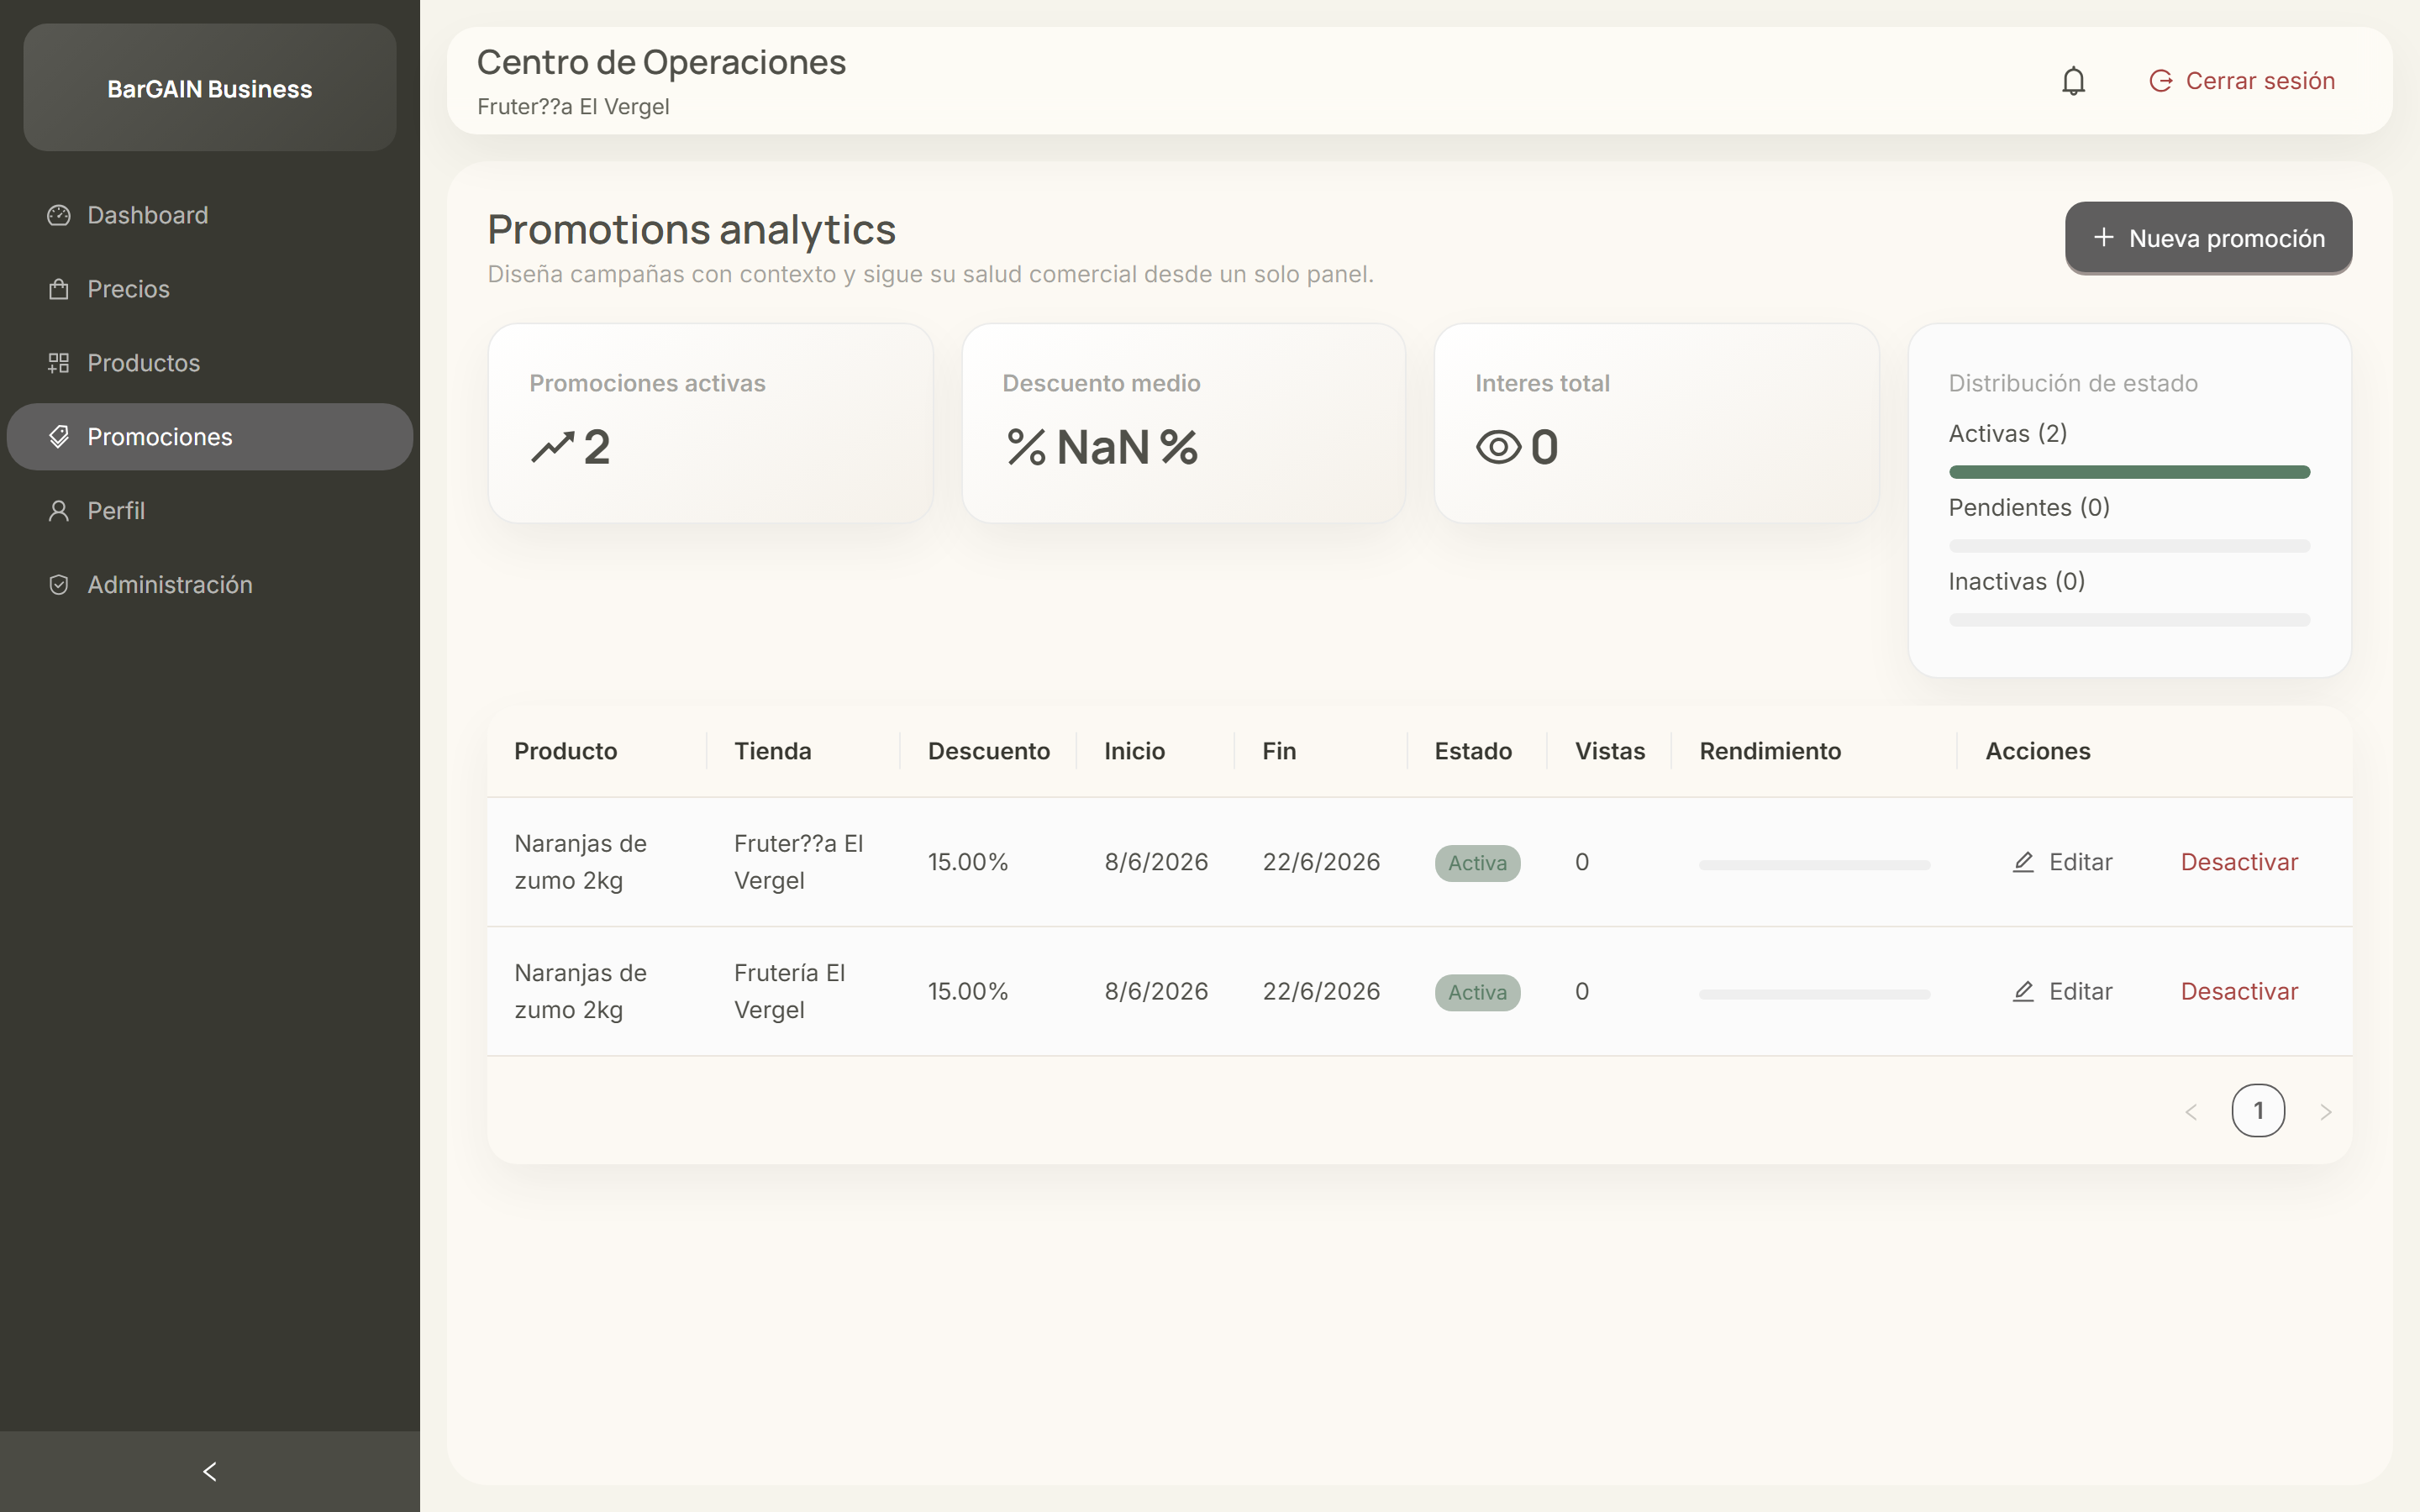
\includegraphics[width=0.46\textwidth]{diagramas/capturas/pyme-promociones.png}
\hfill
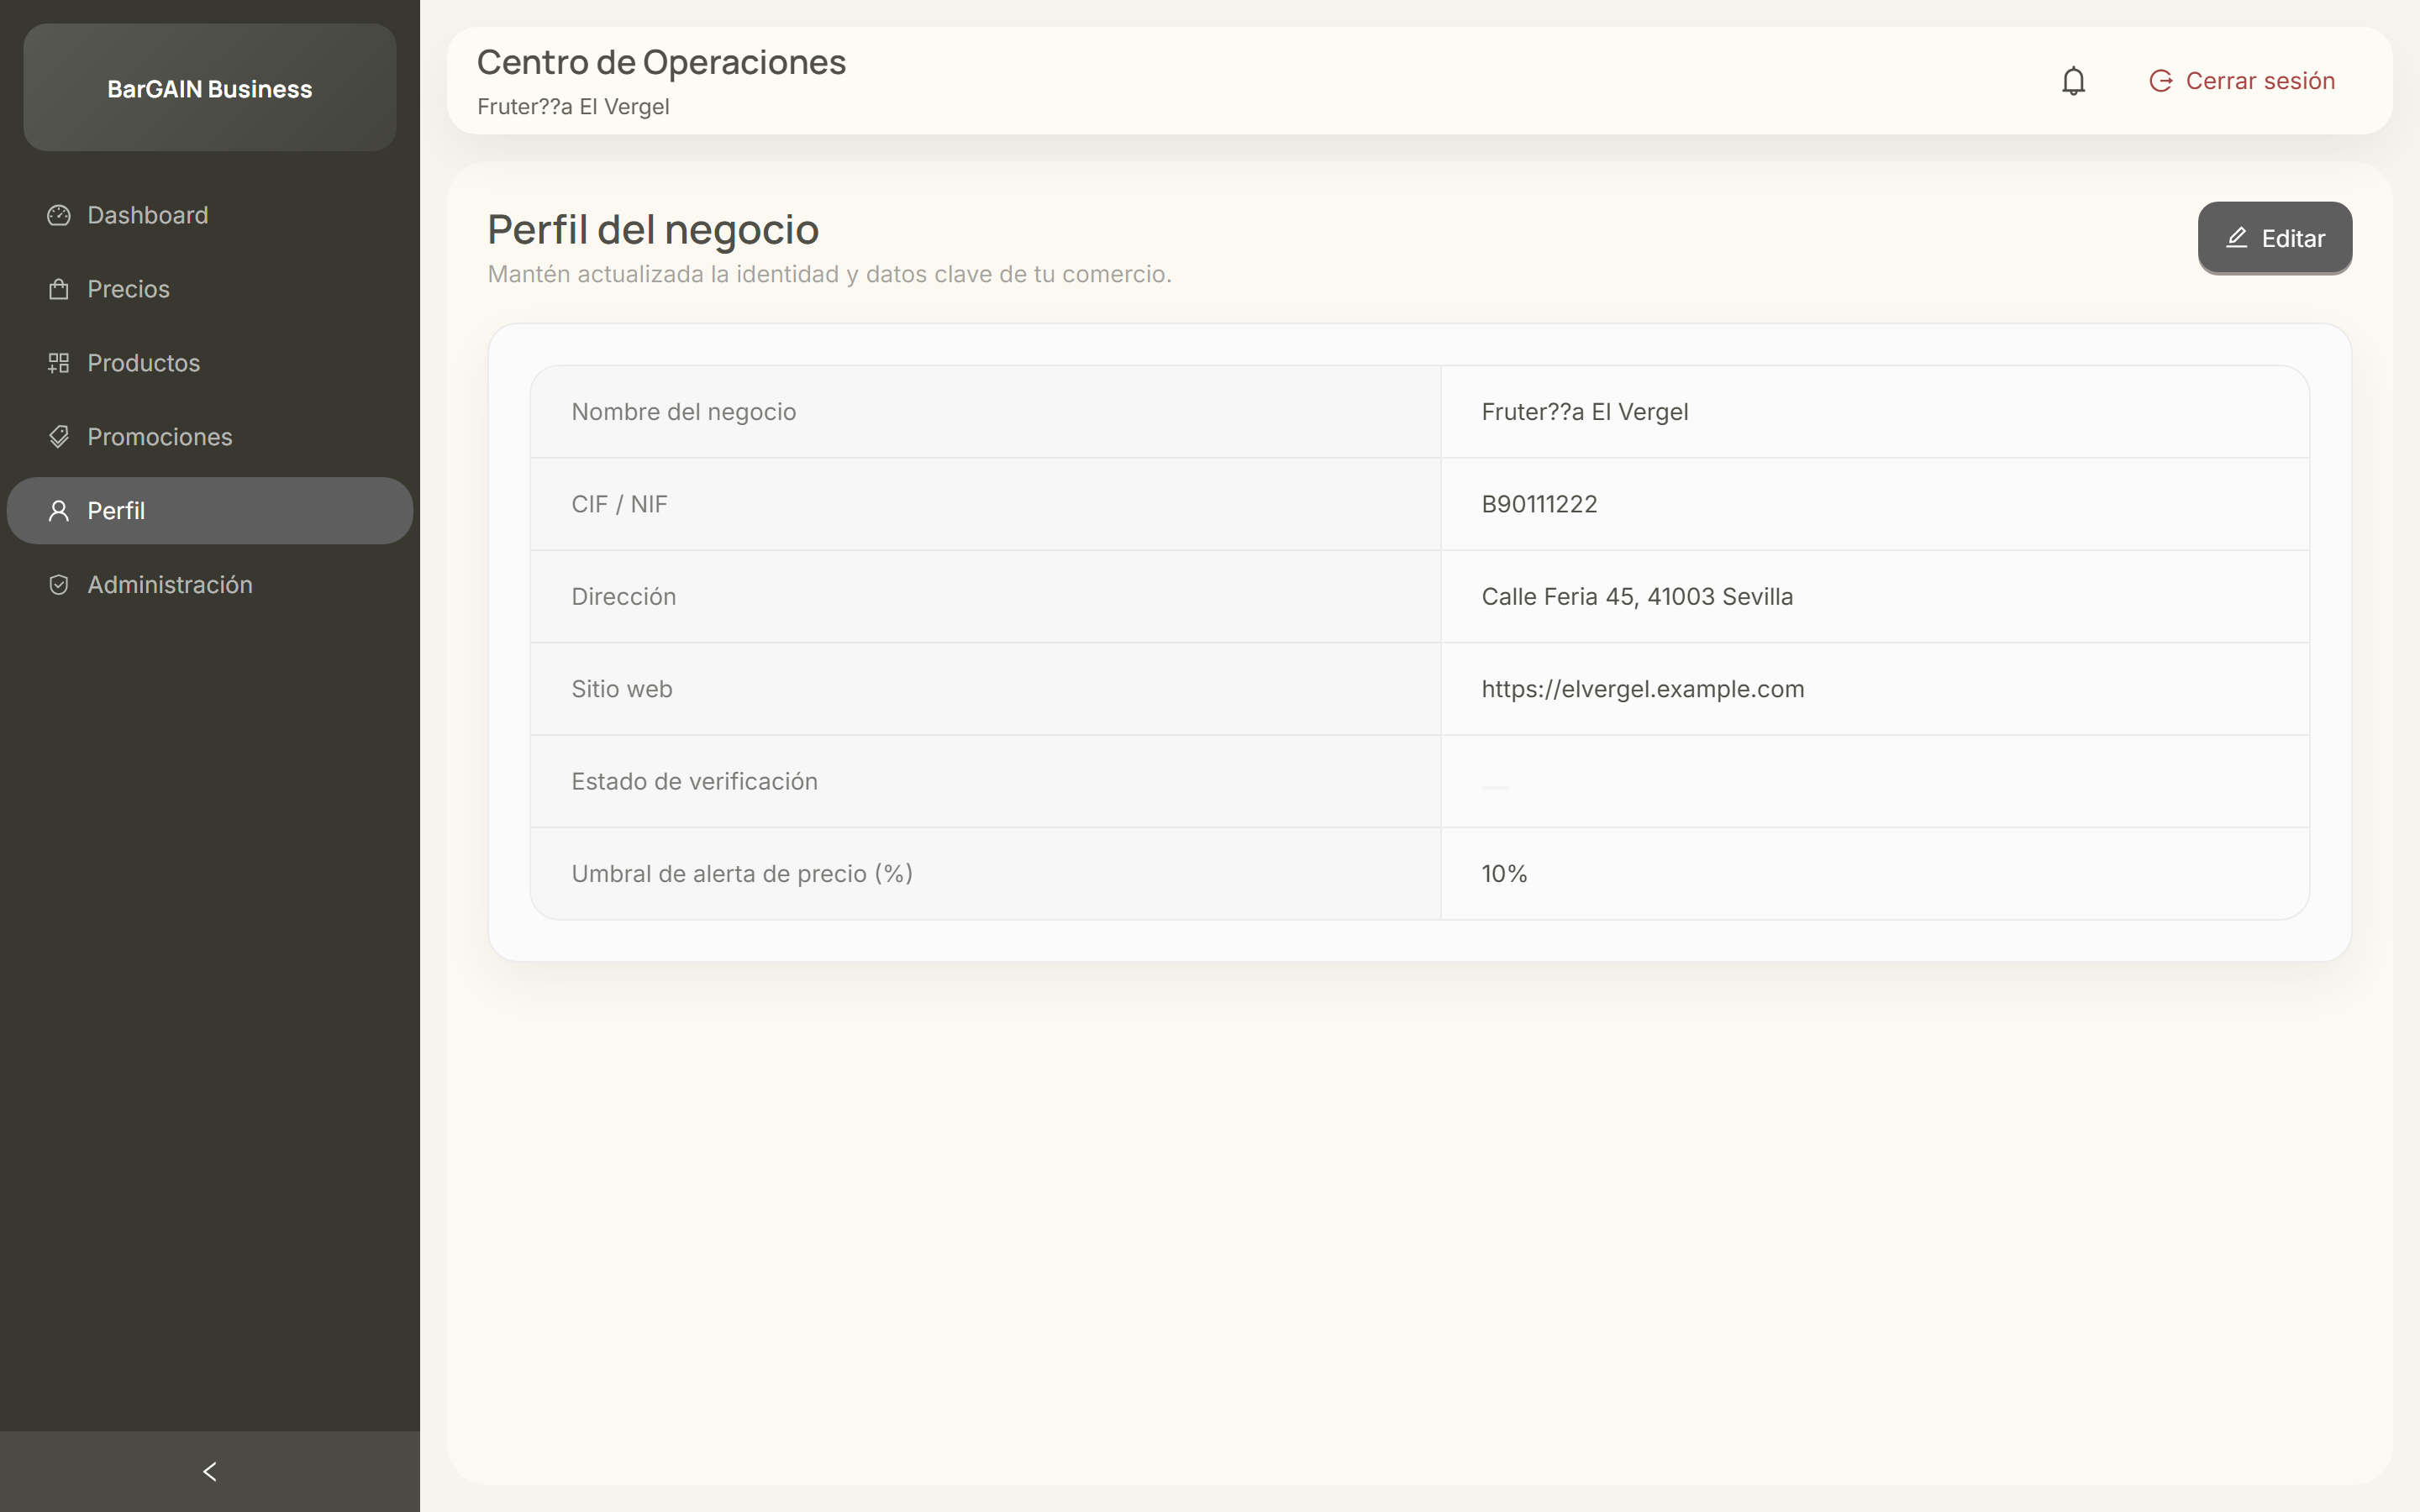
\includegraphics[width=0.46\textwidth]{diagramas/capturas/pyme-perfil-negocio.png}
\caption{Portal PYME --- Gesti\'on de promociones (izquierda) y perfil del negocio (derecha)}
\label{fig:cap-pyme-promo-perfil}
\end{figure}

\begin{figure}[htbp]
\centering
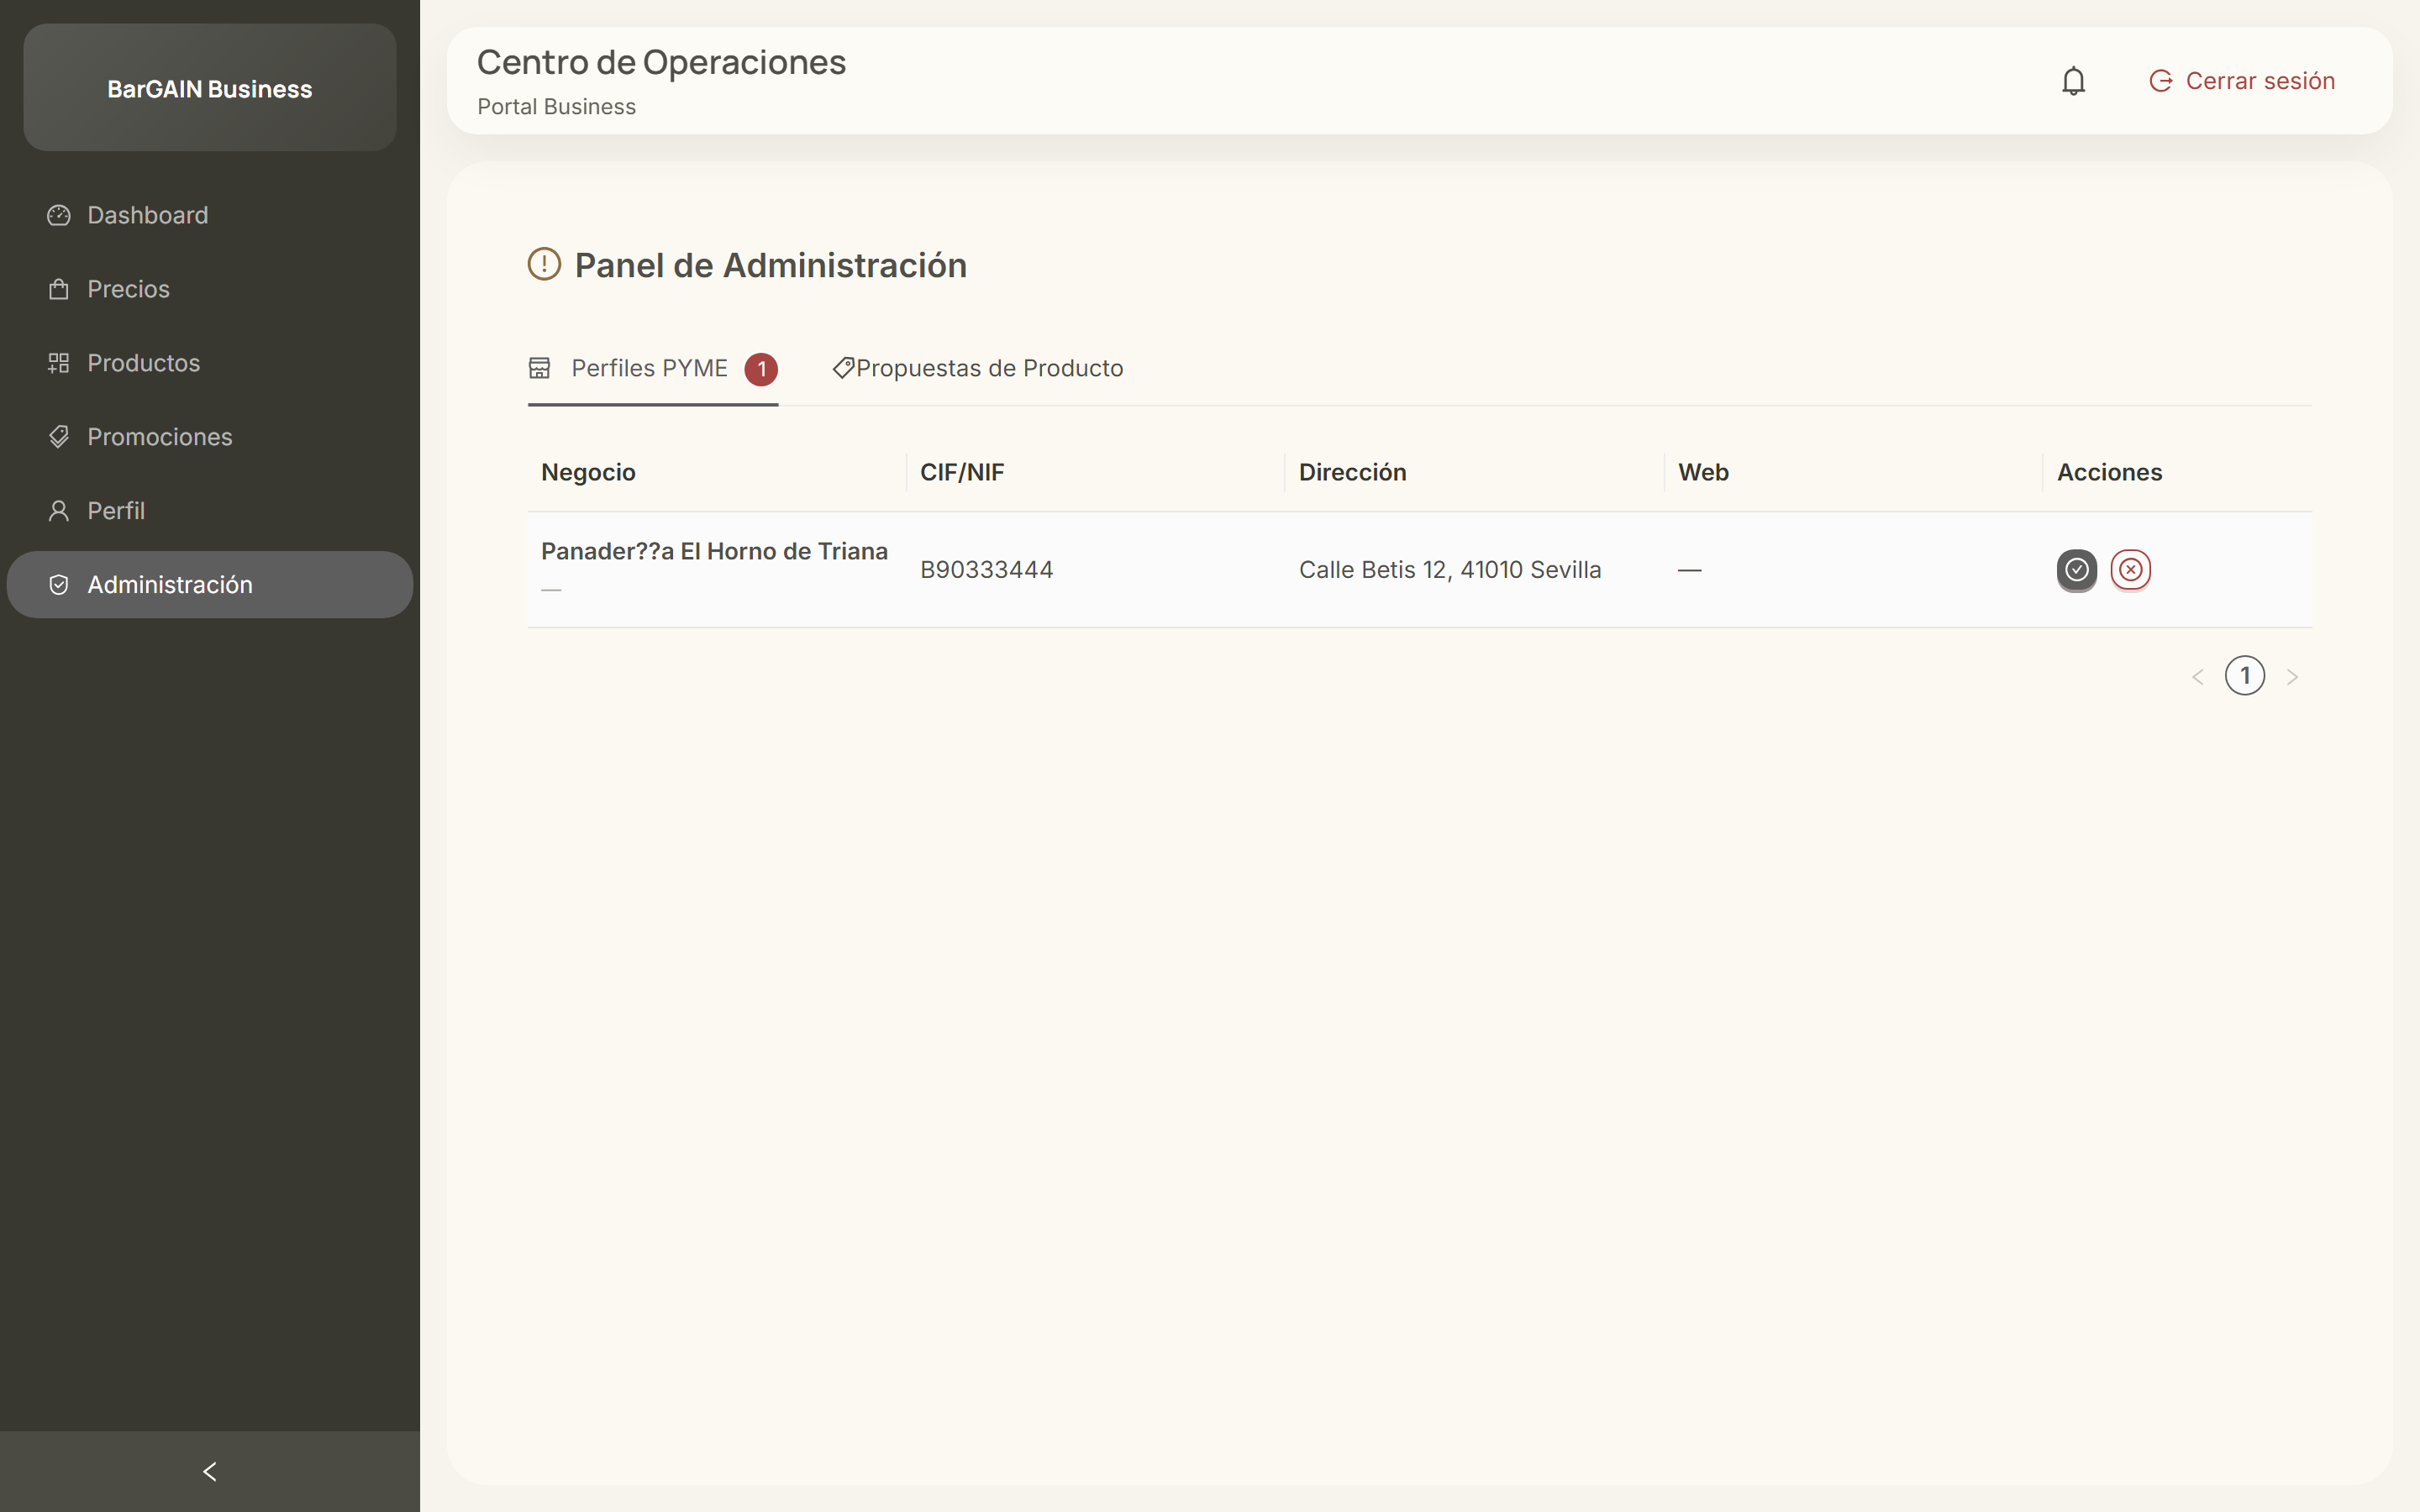
\includegraphics[width=0.85\textwidth]{diagramas/capturas/pyme-admin-aprobacion.png}
\caption{Portal PYME --- Aprobaci\'on de negocios por el administrador}
\label{fig:cap-pyme-admin}
\end{figure}

\clearpage

\section{Resoluci\'on de incidencias comunes}\label{sec:manual-incidencias}

\begin{itemize}
  \item \textbf{Frontend no conecta con backend:} verificar que el backend est\'a levantado
    (\texttt{make dev}) y expuesto en \texttt{http://localhost:8000}.
  \item \textbf{Errores JWT al navegar:} cerrar sesi\'on e iniciar de nuevo para regenerar
    credenciales.
  \item \textbf{No aparecen tiendas en mapa:} comprobar permisos de ubicaci\'on del dispositivo
    o usar coordenadas v\'alidas desde preferencias de perfil.
  \item \textbf{OCR no reconoce texto:} asegurarse de que hay buena iluminaci\'on y el texto es
    legible; usar la opci\'on de galer\'ia con una foto de mayor calidad.
  \item \textbf{Optimizaci\'on muy lenta:} la primera optimizaci\'on tras arrancar el backend puede
    tardar hasta 30 s (cold start en Render free tier). Las siguientes son instant\'aneas porque
    el worker Celery est\'a caliente.
\end{itemize}
